\pdfminorversion=4 % for acroread
\documentclass[t,xcolor={usenames,dvipsnames}]{beamer}
%\documentclass[t,handout,xcolor={usenames,dvipsnames}]{beamer}
\usepackage{beamerstyle}
\usepackage{dsfont}
\usepackage{bm}
\usepackage[english]{babel}
\usepackage[utf8]{inputenc}
\usepackage{graphicx}
\usepackage[boxed,vlined]{algorithm2e}
\usepackage{hyperref}
\usepackage{booktabs}

\usepackage{amsmath,amssymb}
\usepackage{listings}
\lstset{frame=lines,framesep=3pt,numbers=left,numberblanklines=false,basicstyle=\ttfamily\small}

\usepackage{subfig}
\usepackage{multicol}
%\usepackage{appendixnumberbeamer}
%

\usepackage{tikz}
\usetikzlibrary{trees} 
\usetikzlibrary{shapes.geometric}
\usetikzlibrary{positioning,shapes,shadows,arrows,calc,mindmap}
\usetikzlibrary{decorations.pathreplacing}
\usetikzlibrary{intersections}
\pgfdeclarelayer{background}
\pgfdeclarelayer{foreground}
\pgfsetlayers{background,main,foreground}
\tikzstyle{activity}=[rectangle, draw=black, rounded corners, text centered, text width=8em]
\tikzstyle{data}=[rectangle, draw=black, text centered, text width=8em]
\tikzstyle{myarrow}=[->, thick, draw=black]

% Define the layers to draw the diagram
\pgfdeclarelayer{background}
\pgfdeclarelayer{foreground}
\pgfsetlayers{background,main,foreground}

%\usepackage{listings}
%\lstset{numbers=left,
%  showstringspaces=false,
%  frame={tb},
%  captionpos=b,
%  lineskip=0pt,
%  basicstyle=\ttfamily,
%%  extendedchars=true,
%  stepnumber=1,
%  numberstyle=\small,
%  xleftmargin=1em,
%  breaklines
%}

 

\usetheme{Madrid}
%\useinnertheme{rectangles}
\usecolortheme{whale}
\setbeamercolor{alerted text}{fg=blue}
\useoutertheme{infolines}
\setbeamertemplate{navigation symbols}{\vspace{-5pt}} % to lower the logo
\setbeamercovered{invisible}

\makeatletter
\setbeamertemplate{footline}
{
  \leavevmode%
  \hbox{%
  \begin{beamercolorbox}[wd=.333333\paperwidth,ht=2.25ex,dp=1ex,center]{author in head/foot}%
    \usebeamerfont{author in head/foot}\insertshortauthor
  \end{beamercolorbox}%
  \begin{beamercolorbox}[wd=.333333\paperwidth,ht=2.25ex,dp=1ex,center]{title in head/foot}%
    \usebeamerfont{title in head/foot}\insertshorttitle
  \end{beamercolorbox}%
  \begin{beamercolorbox}[wd=.333333\paperwidth,ht=2.25ex,dp=1ex,right]{date in head/foot}%
    \usebeamerfont{date in head/foot}\insertshortdate{}\hspace*{2em}
    \insertframenumber\hspace*{2ex} 
  \end{beamercolorbox}}%
  \vskip0pt%
}
\makeatother

\pgfdeclareimage[height=1.2cm]{automl}{images/logos/automl.png}
\pgfdeclareimage[height=1.2cm]{freiburg}{images/logos/freiburg}

\logo{\pgfuseimage{freiburg}}

\title[AutoML]{Automated Machine Learning}
\subtitle{(AutoML)}
\author{M. Lindauer \and F. Hutter}
\institute{University of Freiburg\\[5em]
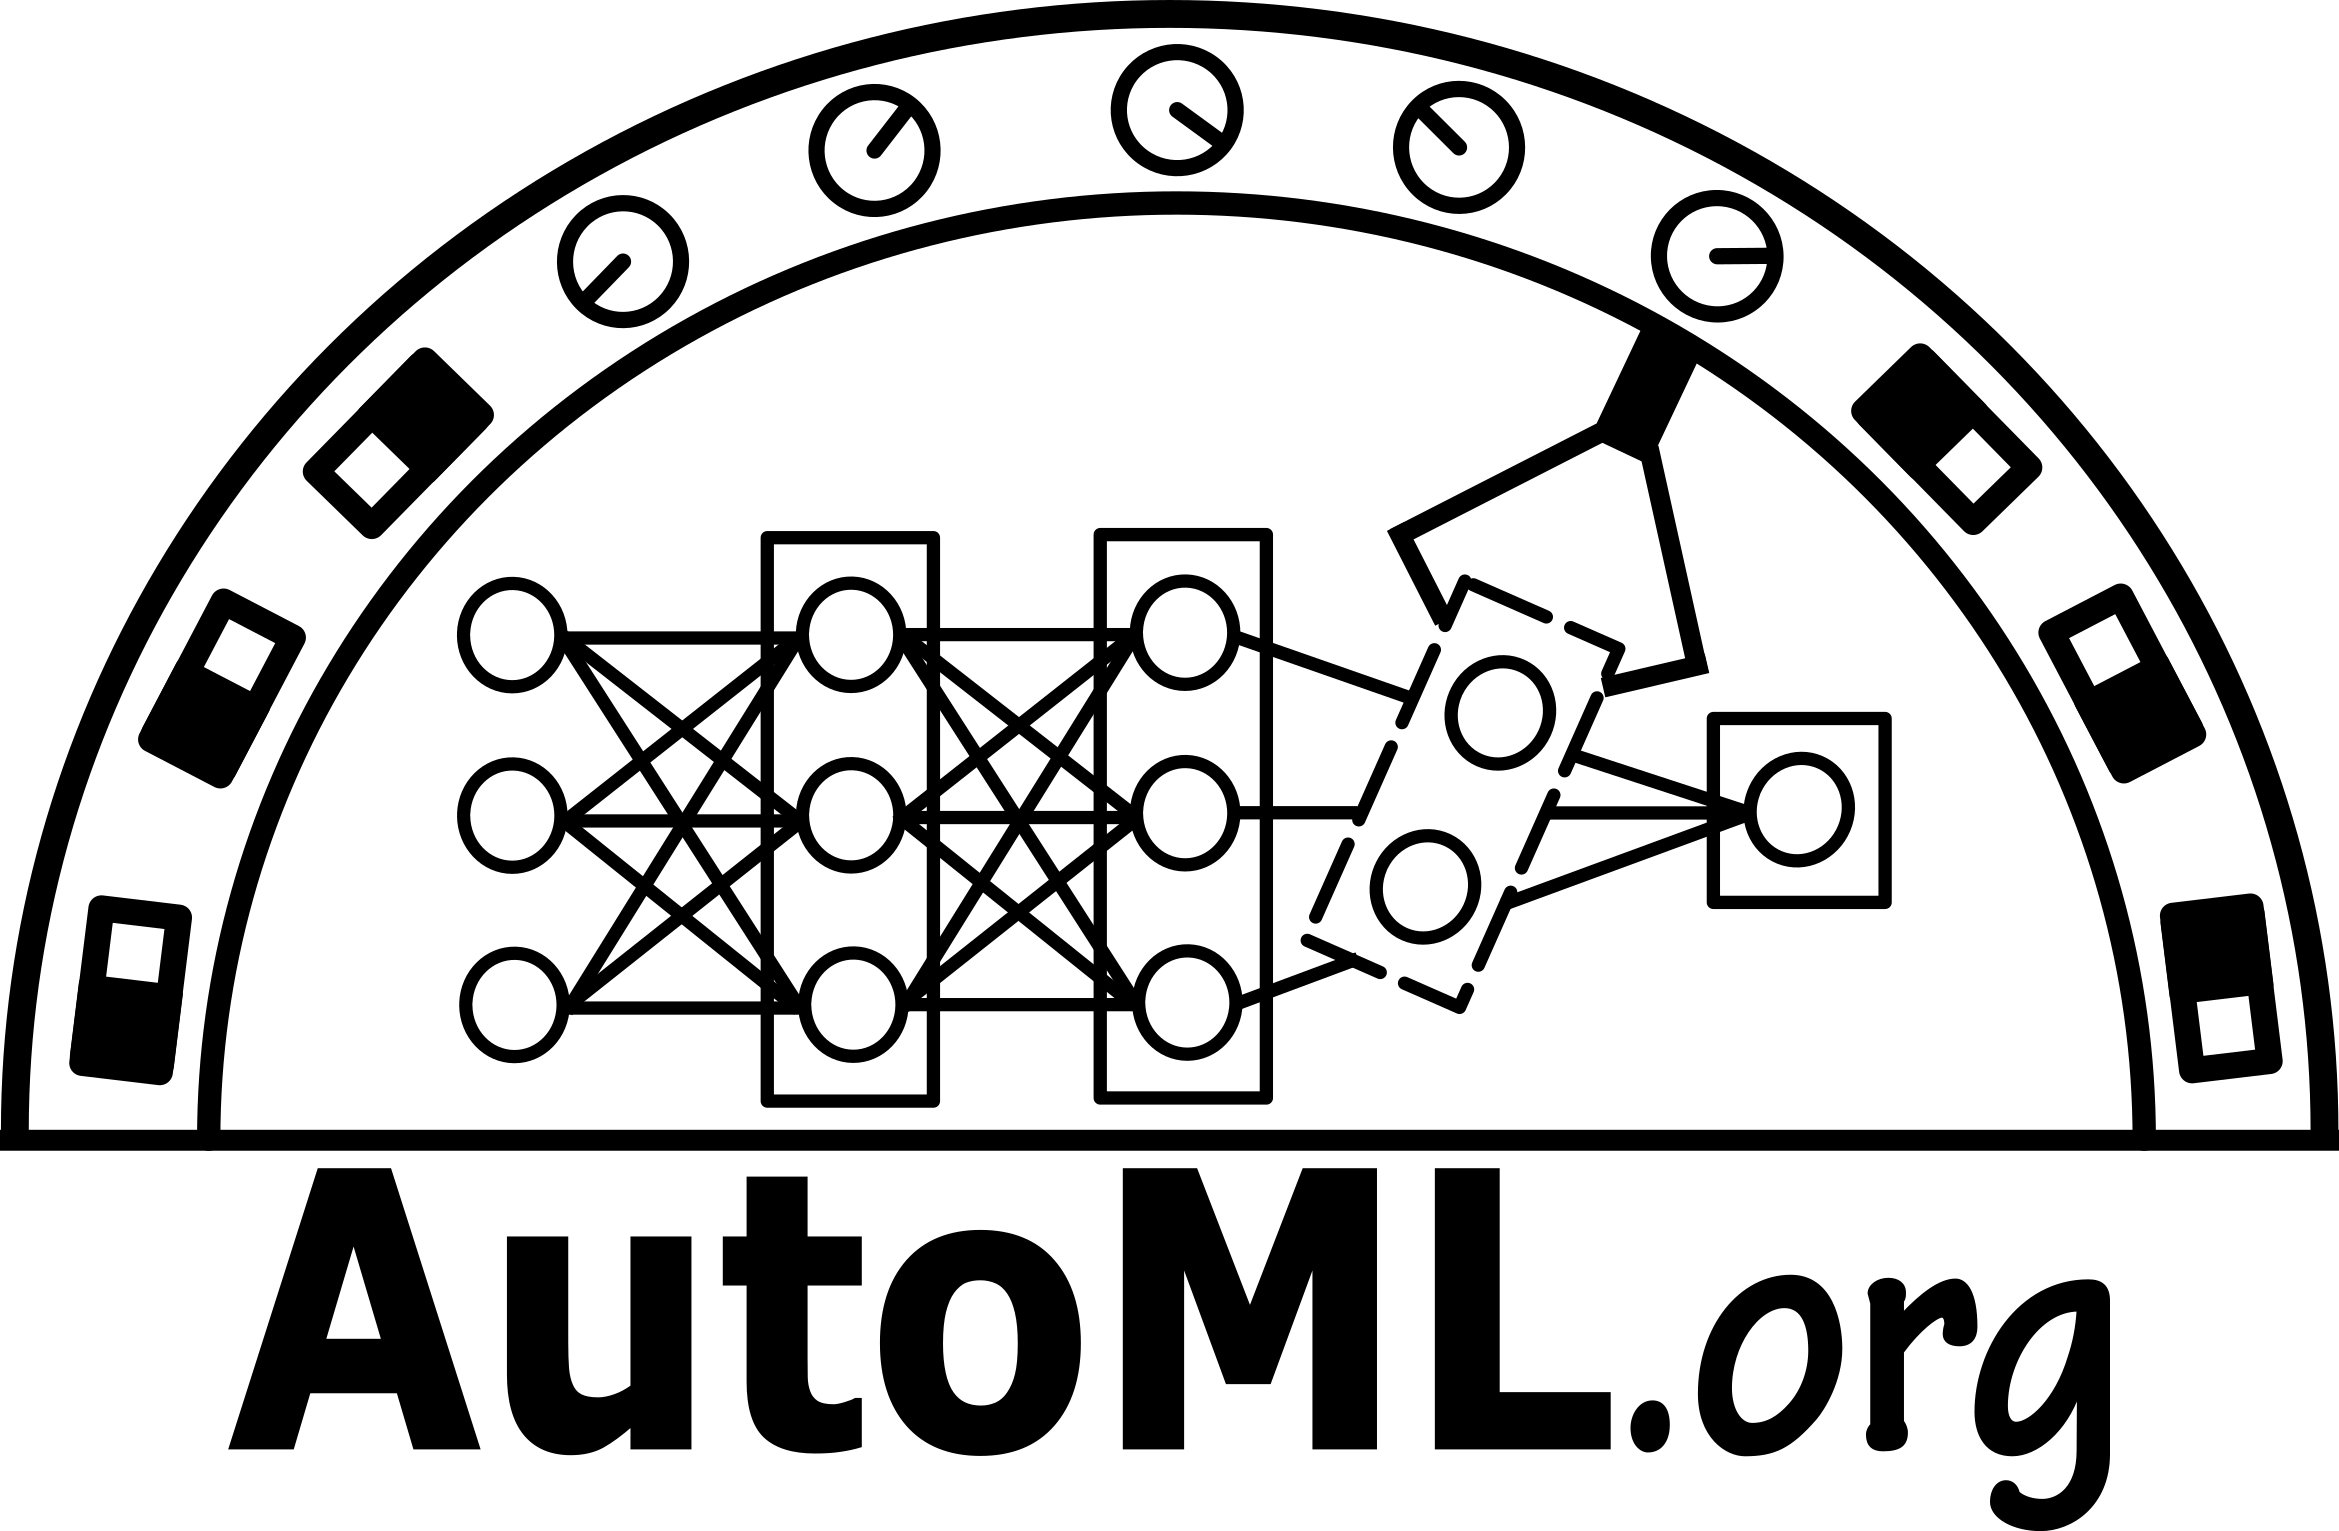
\includegraphics[width=10em]{images/logos/automl}}
\date{}



% \AtBeginSection[] % Do nothing for \section*
% {
%   \begin{frame}{Outline}
%     \bigskip
%     \vfill
%     \tableofcontents[currentsection]
%   \end{frame}
% }

\renewcommand{\comment}[1]{
	\noindent
	%\vspace{0.25cm}
	{\color{red}{\textbf{TODO:} #1}}
	%\vspace{0.25cm}
}
\newcommand{\notefh}[1]{\textcolor{red}{\textbf{FH:} #1}}
\renewcommand{\comment}[1]{}
\newcommand{\hide}[1]{}
\newcommand{\cemph}[2]{\emph{\textcolor{#1}{#2}}}

\newcommand{\lit}[1]{{\footnotesize\color{black!60}[#1]}}

\newcommand{\litw}[1]{{\footnotesize\color{blue!20}[#1]}}


\newcommand{\myframe}[2]{\begin{frame}[c]{#1}#2\end{frame}}
\newcommand{\myframetop}[2]{\begin{frame}{#1}#2\end{frame}}
\newcommand{\myit}[1]{\begin{itemize}#1\end{itemize}}
\newcommand{\myblock}[2]{\begin{block}{#1}#2\end{block}}


\newcommand{\votepurple}[1]{\textcolor{Purple}{$\bigstar$}}
\newcommand{\voteyellow}[1]{\textcolor{Goldenrod}{$\bigstar$}}
\newcommand{\voteblue}[1]{\textcolor{RoyalBlue}{$\bigstar$}}
\newcommand{\votepink}[1]{\textcolor{Pink}{$\bigstar$}}

\newcommand{\diff}{\mathop{}\!\mathrm{d}}
\newcommand{\refstyle}[1]{{\small{\textcolor{gray}{#1}}}}
\newcommand{\hands}[0]{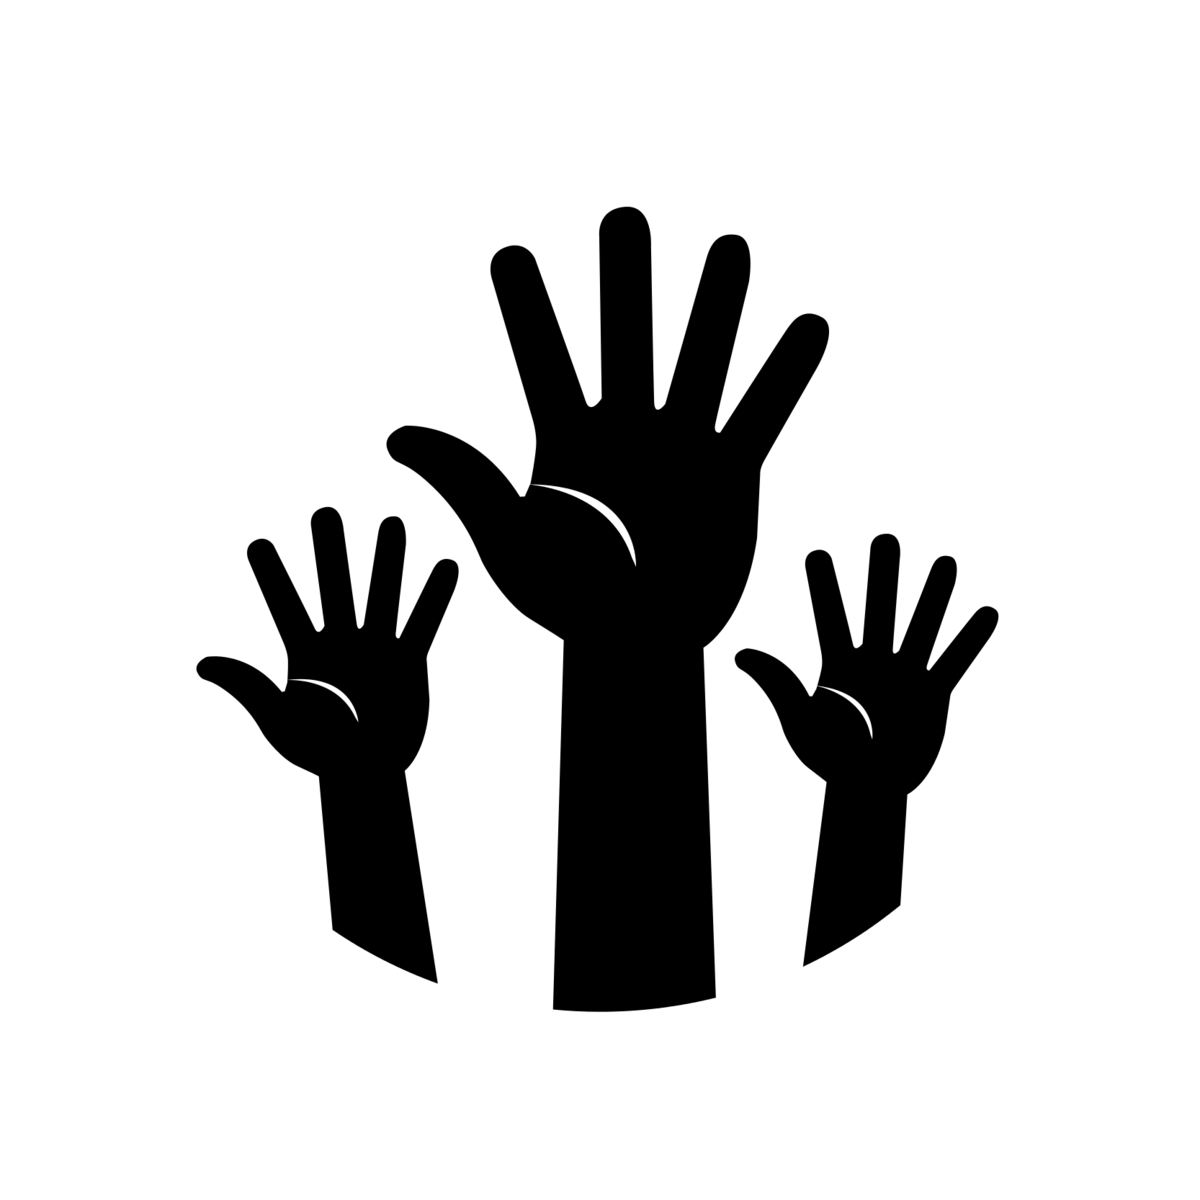
\includegraphics[height=1.5em]{images/hands}}
\newcommand{\transpose}[0]{{\textrm{\tiny{\sf{T}}}}}
\newcommand{\norm}{{\mathcal{N}}}
\newcommand{\cutoff}[0]{\kappa}
\newcommand{\instD}[0]{\dataset}
\newcommand{\insts}[0]{\mathcal{I}}
\newcommand{\inst}[0]{i}
\newcommand{\instI}[1]{i^{(#1)}}

% Iteration specific instance of variable/function/anything
% Introduced in the BO section, but moved up here to make it available within other macros
\newcommand{\iter}[2][\bocount]{{#2}^{(#1)}}

%--------HPO parameter macros-----------

% Parameter Configuration Space
\newcommand{\pcs}[0]{\pmb{\Lambda}}

% ???
\newcommand{\bx}[0]{\conf}

% Parameter Configuration
\newcommand{\conf}[0]{\pmb{\lambda}}

% Final Configuration
\newcommand{\finconf}[0]{\pmb{\hat{\lambda}}}

% Configuration corresponding to a given iteration -- better use \iter!
\newcommand{\confI}[1]{{\conf}^{(#1)}}

% Default Configuration
\newcommand{\defconf}[0]{{\conf}_{\text{def}}}

% Incumbent Configuration
\newcommand{\incumbent}[1][\bocount]{\iter[#1]{\finconf}}

% Optimal Configuration
\newcommand{\optconf}[0]{{\conf}^*}

% Configuration Space
\newcommand{\confs}[0]{\pcs}

%----------------------------------------

%\newcommand{\vlambda}[0]{\bm{\lambda}}
%\newcommand{\vLambda}[0]{\bm{\Lambda}}
\newcommand{\dataset}[0]{\mathcal{D}}
\newcommand{\datasets}[0]{\mathbf{D}}
\newcommand{\loss}[0]{L}
\newcommand{\risk}{\mathcal{R}}
\newcommand{\riske}{\mathcal{R}_{\text{emp}}}
\newcommand{\cost}[0]{c}
\newcommand{\costI}[1]{c^{(#1)}}

% Gaussian Process
\newcommand{\gp}{\mathcal{G}}
% Family of Objective Functions
\newcommand{\objF}{F}

%---------------BO Macros------------------

% BO loop counter
\newcommand{\bocount}{t}
% BO loop counter max, the counter runs from 1 to this value
\newcommand{\bobudget}{T}
% BO loop observation
\newcommand{\obs}[1][\conf]{\cost({#1})}
% BO loop observation space
\newcommand{\obsspace}{\mathcal{Y}}
% BO loop next observation
\newcommand{\bonextobs}{\obs[\iter{\conf}]}
% Acquisition Function, no args
\newcommand{\acq}{u}
% Standard Normal PDF
\newcommand{\pdf}{\phi}
% Standard Normal CDF
\newcommand{\cdf}{\Phi}
% Mean
\newcommand{\mean}{\mu}
% Standard Deviation
\newcommand{\stddev}{\sigma}
% Variance
\newcommand{\variance}{\sigma^2}
% Noise
\newcommand{\noise}{\nu}
% BO loop next selected sample
\newcommand{\bonextsample}{\confI{\bocount}}

% Single hyperparameter
\newcommand{\hyperparam}{\lambda}

% Single hyperparameter within a hyperparameter configuration
\newcommand{\hyperparami}[1][i]{{\hyperparam}_#1}

% Full definition of final configuration
\newcommand{\finconffull}{\incumbent[\bobudget]}

% Dataset
\newcommand{\datasetHPO}{{\dataset}_{HPO}}

% Dataset definition
\newcommand{\datasetHPOdef}{{\langle \bonextsample,\,\bonextobs \rangle}_{\bocount=1}^{\bobudget}}

% Double Display Fraction, forces large displays for everything in numerator and denominator
\newcommand\ddfrac[2]{\frac{\displaystyle #1}{\displaystyle #2}}

% Conditional Probability "Given That" Relation, source:https://tex.stackexchange.com/a/141685/205886
\newcommand\given[1][]{\:#1\vert\:}

% Expectation as a math operator
\DeclareMathOperator*{\E}{\mathbb{E}}

% Citation 
\newcommand{\source}[1]{
    \begin{flushright}
    	Source: \lit{#1}
    \end{flushright}
}
%-------------------------------------------

%Real numbers set
\newcommand{\realnum}{\mathbb{R}}
%Configuration space - do not use
%\newcommand{\configspace}{\Theta}
%Instances - do not use
%\newcommand{\instances}{\mathcal{I}}
%Expected value
\newcommand{\expectation}{\mathbb{E}}
%Kernel
\newcommand{\kernel}{\kappa}
%Constraint function
\newcommand{\constraintf}{c}
%Normal distribution
\newcommand{\normaldist}{\mathcal{N}}

% \renewcommand{\vec}[1]{\mathbf{#1}}
\newcommand{\hist}[0]{\dataset_{\text{Hist}}}
\newcommand{\param}[0]{p}
\newcommand{\algo}[0]{\mathcal{A}}
\newcommand{\algos}[0]{\mathbf{A}}
%\newcommand{\nn}[0]{N}
\newcommand{\feats}[0]{\mathcal{X}_{\text{meta}}}
\newcommand{\feat}[0]{\x_{\text{meta}}}
%\newcommand{\cluster}[0]{\vec{h}}
%\newcommand{\clusters}[0]{\vec{H}}
\newcommand{\perf}[0]{\mathbb{R}}
%\newcommand{\surro}[0]{\mathcal{S}}
\newcommand{\surro}[0]{\hat{\cost}}
\newcommand{\func}[0]{f}
\newcommand{\epm}[0]{\surro}
\newcommand{\portfolio}[0]{\mathbf{P}}
\newcommand{\schedule}[0]{\mathcal{S}}

% Machine Learning
\newcommand{\mdata}[0]{\dataset_{\text{meta}}}
\newcommand{\datasettrain}[0]{\dataset_{\text{train}}}
\newcommand{\datasetval}[0]{\dataset_{\text{val}}}
\newcommand{\datasettest}[0]{\dataset_{\text{test}}}
\newcommand{\x}[0]{\mathbf{x}}
\newcommand{\y}[0]{y}
\newcommand{\xI}[1]{\mathbf{x}^{(#1)}}
\newcommand{\yI}[1]{y^{(#1)}}
\newcommand{\fx}{f(\mathbf{x})}  % f(x), continuous prediction function
\newcommand{\Hspace}{\mathcal{H}} % hypothesis space where f is from
\newcommand{\fh}{\hat{f}}       % f hat, estimated prediction function

% Deep Learning
\newcommand{\weights}[0]{\theta}
\newcommand{\metaweights}[0]{\phi}


% reinforcement learning
\newcommand{\policies}[0]{\mathbf{\Pi}}
\newcommand{\policy}[0]{\pi}
\newcommand{\actionRL}[0]{a}
\newcommand{\stateRL}[0]{s}
\newcommand{\statesRL}[0]{\mathcal{S}}
\newcommand{\rewardRL}[0]{r}
\newcommand{\rewardfuncRL}[0]{\mathcal{R}}

\RestyleAlgo{algoruled}
\DontPrintSemicolon
\LinesNumbered
\SetAlgoVlined
\SetFuncSty{textsc}

\SetKwInOut{Input}{Input}
\SetKwInOut{Output}{Output}
\SetKw{Return}{return}

%\newcommand{\changed}[1]{{\color{red}#1}}

%\newcommand{\citeN}[1]{\citeauthor{#1}~(\citeyear{#1})}

\renewcommand{\vec}[1]{\mathbf{#1}}
\DeclareMathOperator*{\argmin}{arg\,min}
\DeclareMathOperator*{\argmax}{arg\,max}

%\newcommand{\aqme}{\textit{AQME}}
%\newcommand{\aslib}{\textit{ASlib}}
%\newcommand{\llama}{\textit{LLAMA}}
%\newcommand{\satzilla}{\textit{SATzilla}}
%\newcommand{\satzillaY}[1]{\textit{SATzilla'{#1}}}
%\newcommand{\snnap}{\textit{SNNAP}}
%\newcommand{\claspfolioTwo}{\textit{claspfolio~2}}
%\newcommand{\flexfolio}{\textit{FlexFolio}}
%\newcommand{\claspfolioOne}{\textit{claspfolio~1}}
%\newcommand{\isac}{\textit{ISAC}}
%\newcommand{\eisac}{\textit{EISAC}}
%\newcommand{\sss}{\textit{3S}}
%\newcommand{\sunny}{\textit{Sunny}}
%\newcommand{\ssspar}{\textit{3Spar}}
%\newcommand{\cshc}{\textit{CSHC}}
%\newcommand{\cshcpar}{\textit{CSHCpar}}
%\newcommand{\measp}{\textit{ME-ASP}}
%\newcommand{\aspeed}{\textit{aspeed}}
%\newcommand{\autofolio}{\textit{AutoFolio}}
%\newcommand{\cedalion}{\textit{Cedalion}}
\newcommand{\fanova}{\textit{fANOVA}}
\newcommand{\sbs}{\textit{SB}}
\newcommand{\oracle}{\textit{VBS}}

% like approaches
\newcommand{\claspfoliolike}[1]{\texttt{claspfolio-#1-like}}
\newcommand{\satzillalike}[1]{\texttt{SATzilla'#1-like}}
\newcommand{\isaclike}{\texttt{ISAC-like}}
\newcommand{\ssslike}{\texttt{3S-like}}
\newcommand{\measplike}{\texttt{ME-ASP-like}}

\newcommand{\irace}{\textit{I/F-race}}
\newcommand{\gga}{\textit{GGA}}
\newcommand{\smac}{\textit{SMAC}}
\newcommand{\paramils}{\textit{ParamILS}}
\newcommand{\spearmint}{\textit{Spearmint}}
\newcommand{\tpe}{\textit{TPE}}


\usepackage{pifont}
\newcommand{\itarrow}{\mbox{\Pisymbol{pzd}{229}}}
\newcommand{\ithook}{\mbox{\Pisymbol{pzd}{52}}}
\newcommand{\itcross}{\mbox{\Pisymbol{pzd}{56}}}
\newcommand{\ithand}{\mbox{\raisebox{-1pt}{\Pisymbol{pzd}{43}}}}

%\DeclareMathOperator*{\argmax}{arg\,max}

\newcommand{\ie}{{\it{}i.e.\/}}
\newcommand{\eg}{{\it{}e.g.\/}}
\newcommand{\cf}{{\it{}cf.\/}}
\newcommand{\wrt}{\mbox{w.r.t.}}
\newcommand{\vs}{{\it{}vs\/}}
\newcommand{\vsp}{{\it{}vs\/}}
\newcommand{\etc}{{\copyedit{etc.}}}
\newcommand{\etal}{{\it{}et al.\/}}

\newcommand{\pscProc}{{\bf procedure}}
\newcommand{\pscBegin}{{\bf begin}}
\newcommand{\pscEnd}{{\bf end}}
\newcommand{\pscEndIf}{{\bf endif}}
\newcommand{\pscFor}{{\bf for}}
\newcommand{\pscEach}{{\bf each}}
\newcommand{\pscThen}{{\bf then}}
\newcommand{\pscElse}{{\bf else}}
\newcommand{\pscWhile}{{\bf while}}
\newcommand{\pscIf}{{\bf if}}
\newcommand{\pscRepeat}{{\bf repeat}}
\newcommand{\pscUntil}{{\bf until}}
\newcommand{\pscWithProb}{{\bf with probability}}
\newcommand{\pscOtherwise}{{\bf otherwise}}
\newcommand{\pscDo}{{\bf do}}
\newcommand{\pscTo}{{\bf to}}
\newcommand{\pscOr}{{\bf or}}
\newcommand{\pscAnd}{{\bf and}}
\newcommand{\pscNot}{{\bf not}}
\newcommand{\pscFalse}{{\bf false}}
\newcommand{\pscEachElOf}{{\bf each element of}}
\newcommand{\pscReturn}{{\bf return}}

%\newcommand{\param}[1]{{\sl{}#1}}
\newcommand{\var}[1]{{\it{}#1}}
\newcommand{\cond}[1]{{\sf{}#1}}
%\newcommand{\state}[1]{{\sf{}#1}}
%\newcommand{\func}[1]{{\sl{}#1}}
\newcommand{\set}[1]{{\Bbb #1}}
%\newcommand{\inst}[1]{{\tt{}#1}}
\newcommand{\myurl}[1]{{\small\sf #1}}

\newcommand{\Nats}{{\Bbb N}}
\newcommand{\Reals}{{\Bbb R}}
\newcommand{\extset}[2]{\{#1 \; | \; #2\}}

\newcommand{\vbar}{$\,\;|$\hspace*{-1em}\raisebox{-0.3mm}{$\,\;\;|$}}
\newcommand{\vendbar}{\raisebox{+0.4mm}{$\,\;|$}}
\newcommand{\vend}{$\,\:\lfloor$}


\newcommand{\goleft}[2][.7]{\parbox[t]{#1\linewidth}{\strut\raggedright #2\strut}}
\newcommand{\rightimage}[2][.3]{\mbox{}\hfill\raisebox{1em-\height}[0pt][0pt]{\includegraphics[width=#1\linewidth]{#2}}\vspace*{-\baselineskip}}

\usepackage{mathtools}

\begin{document}

\maketitle

%\begin{frame}[c]{In a Nutshell}

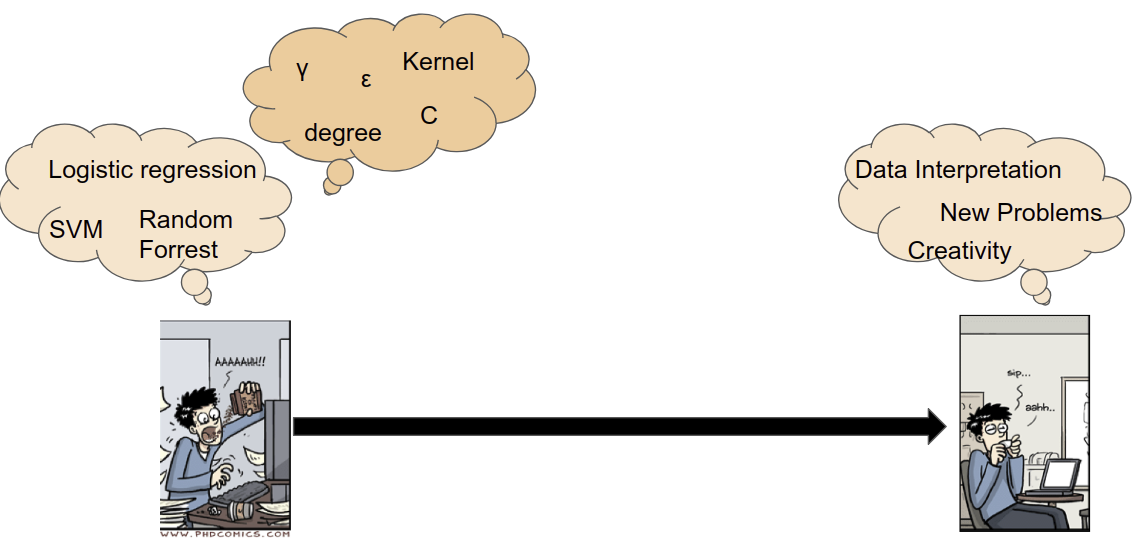
\includegraphics[width=0.99\textwidth]{images/automl_comic}

\end{frame}
%----------------------------------------------------------------------
%----------------------------------------------------------------------
\begin{frame}[c]{}

\huge
\centering
Why are you sitting here?

\bigskip

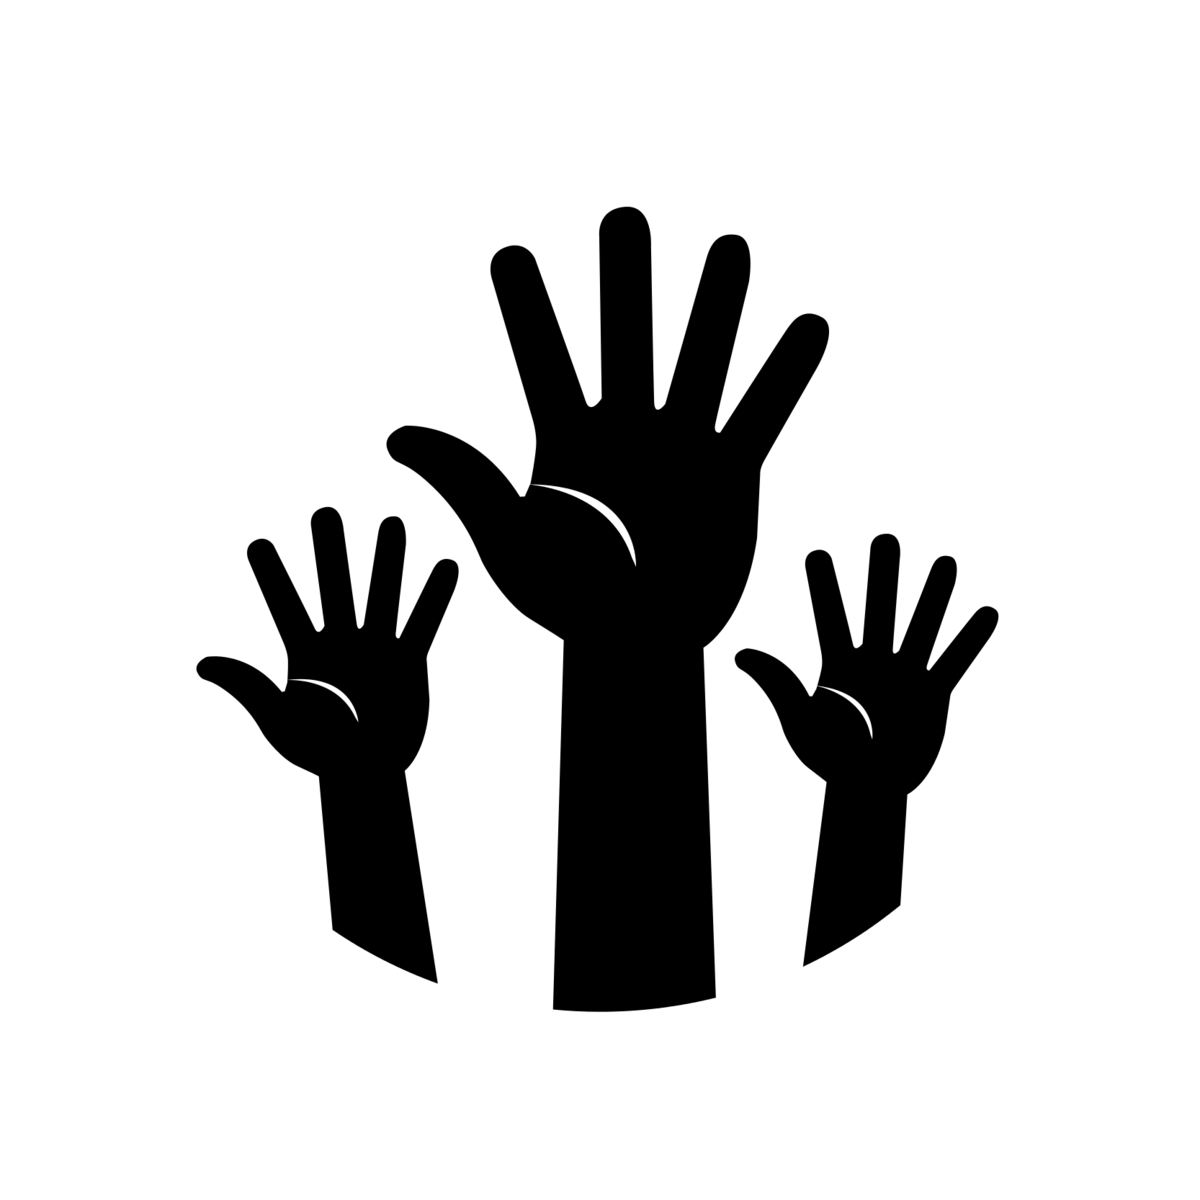
\includegraphics[scale=0.1]{images/hands.png}

\end{frame}
%----------------------------------------------------------------------
\begin{frame}[c]{}

\centering
\huge
Lecture 1:\\
Overview and Motivation
\end{frame}
%----------------------------------------------------------------------
%----------------------------------------------------------------------
\begin{frame}[c]{Overview}

What do we learn today?

\begin{itemize}
  \item Why ML does not scale up
  \item Design decisions in ML 
  \item What is AutoML? 
  \item Challenges in AutoML
  \item Risks of AutoML
  \item Meta-algorithmic hierarchy 
  \item Organization of the course
\end{itemize}

\end{frame}
%-----------------------------------------------------------------------
%----------------------------------------------------------------------
\begin{frame}[c]{Machine Learning}

\centering
\textit{``Machine learning is the science of getting computers to act\\
 without being explicitly programmed.''}

\hfill by Andrew Ng

\end{frame}
%-----------------------------------------------------------------------
%----------------------------------------------------------------------
\begin{frame}[c]{Machine Learning}

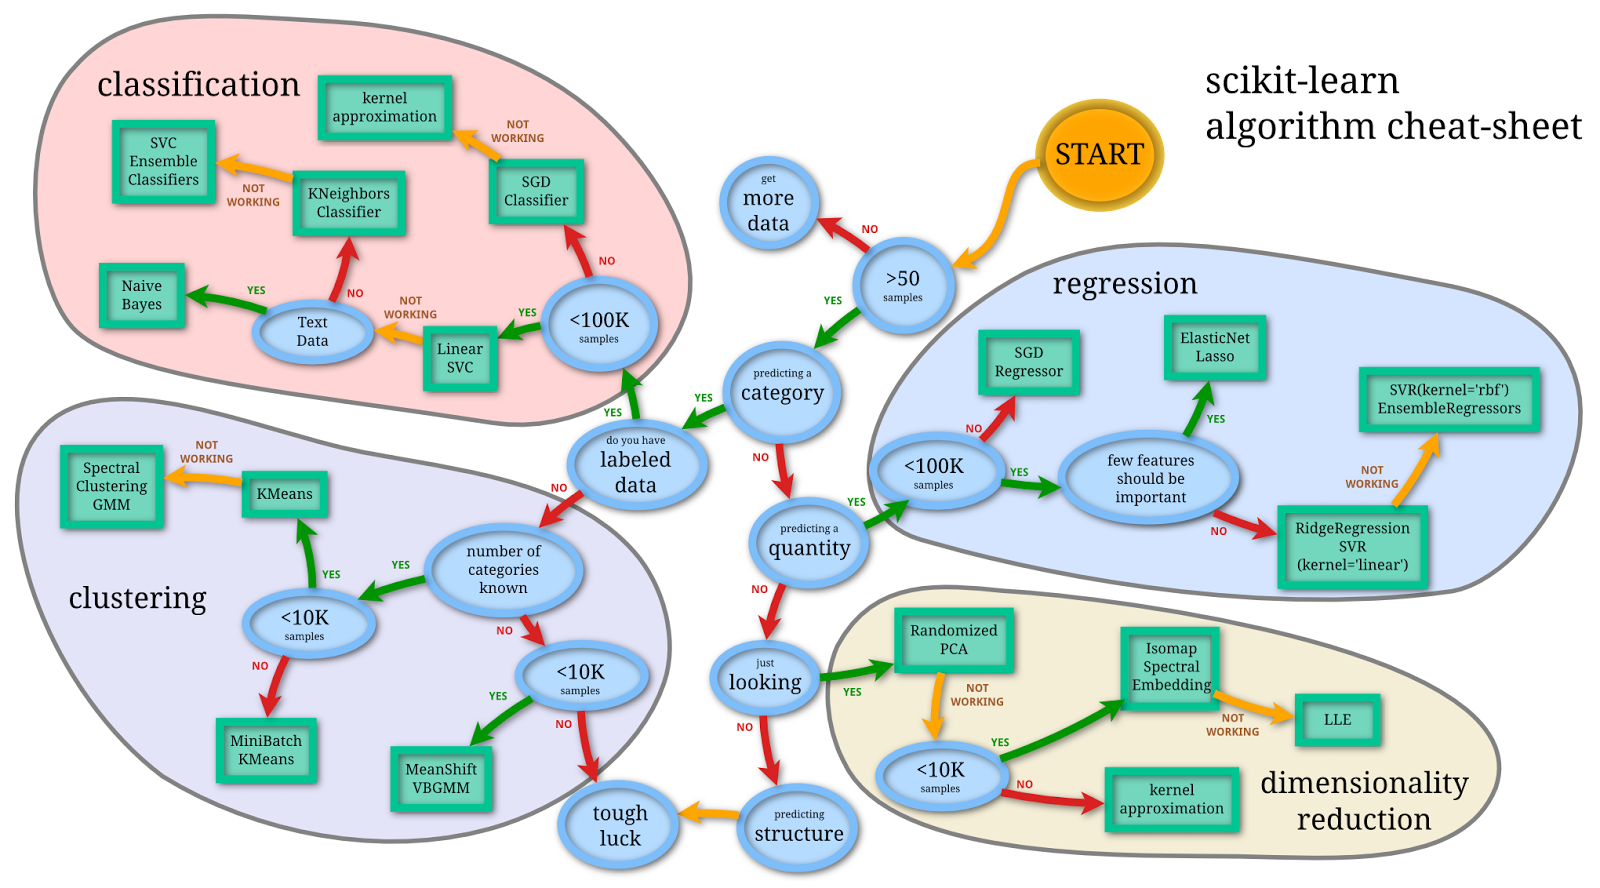
\includegraphics[width=1.0\textwidth]{images/sklearn-cheat}

\end{frame}
%-----------------------------------------------------------------------
%----------------------------------------------------------------------
\begin{frame}[c]{Machine Learning Workflow}

\centering
\tikzstyle{activity}=[rectangle, draw=black, rounded corners, text centered, text width=8em, fill=white, drop shadow]
\tikzstyle{wideactivity}=[rectangle, draw=black, rounded corners, text centered, text width=10em, fill=white, drop shadow]
\tikzstyle{data}=[rectangle, draw=black, text centered, fill=black!10, text width=8em, drop shadow]
\tikzstyle{myarrow}=[->, thick]
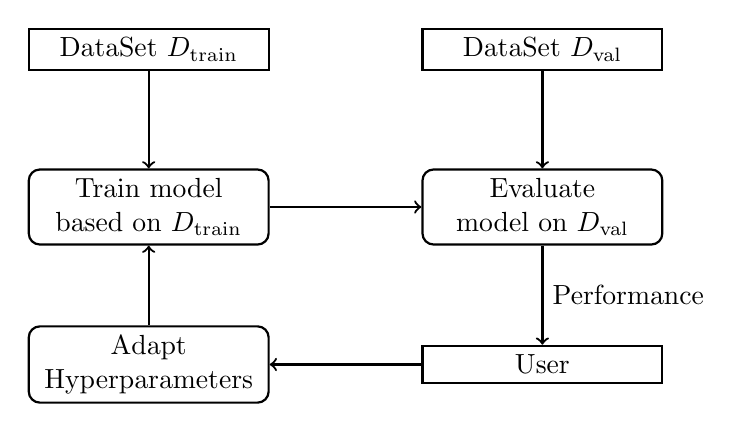
\begin{tikzpicture}[node distance=5cm,thick]
	\node (Train) [data] {DataSet $D_{\text{train}}$};
	\node (Fit) [activity, below of=Train, node distance=2cm] {Train model based on $D_{\text{train}}$};
	\draw[myarrow] (Train) -- (Fit);
	
	\pause
	
	\node (Test) [data, right of=Train] {DataSet $D_{\text{val}}$};
	\node (Eva) [activity, below of=Test, node distance=2cm] {Evaluate model on $D_{\text{val}}$};
	\draw[myarrow] (Fit) -- (Eva);
	\draw[myarrow] (Test) -- (Eva);
	
	\pause
	
	\node (user) [data, below of=Eva, node distance=2cm] {User};
	\draw[myarrow] (Eva) to node[right] {Performance} (user);
	
	\pause
	
	\node (Hyper) [activity, left of=user] {Adapt\\ Hyperparameters};
	\draw[myarrow] (user) to (Hyper);
	\draw[myarrow] (Hyper) to (Fit);
	
\end{tikzpicture}


\pause
 
\bigskip
\bigskip
$\leadsto$ Users indirectly teach machines how to learn.

\end{frame}
%-----------------------------------------------------------------------
%----------------------------------------------------------------------
\begin{frame}[c]{Machine Learning does not scale up}

\begin{itemize}
  \item Basics in machine learning are not hard to grasp
  \smallskip
  \item Achieving state-of-the-art performance is quite hard
  \smallskip
  \item Design decisions are (sometimes) unintuitive and\\ require a lot of expertise
  \begin{itemize}
    \item making these design decisions is a tedious and error-prone task
  \end{itemize}
  \smallskip
  \item Many experts are employed in ML these days
  \smallskip
  \item Nevertheless, developing a new ML-applications takes time
  \smallskip
  \item The job market for ML experts is nearly empty
\end{itemize}

\bigskip

\textit{``I'd like to use machine learning, but I can't invest much time''}

\hfill Zoubin Gharamani


\end{frame}
%-----------------------------------------------------------------------
%----------------------------------------------------------------------
\begin{frame}[c]{Design Decisions in Machine Learning}

What could be design decisions for applying ML to a new dataset?
\hands

\pause

\begin{itemize}
  \item Choice of machine learning algorithm
  \begin{itemize}
    \item SVM, random forest, deep neural network?
  \end{itemize}
  \pause
  \item Hyperparameters of machine learning algorithms
  \begin{itemize}
    \item SVM: C, gamma, kernel, \ldots?
  \end{itemize}
  \pause
  \item Architecture of a neural network
  \begin{itemize}
    \item $\#$layers, $\#$neurons, activation function, \ldots 
  \end{itemize}
  \pause
  \item Data preprocessing
  \begin{itemize}
  	\item data cleanup, missing data imputation, feature selection, \ldots  
  \end{itemize}
  \pause
  \item anomaly detection
  \item allocation of computational resources
  \item \ldots
\end{itemize}

\medskip
$\leadsto$ All these design decisions have to be made for each new dataset.

\end{frame}
%-----------------------------------------------------------------------
%----------------------------------------------------------------------
\begin{frame}[c]{A simple Example with $k$-NN}

\centering
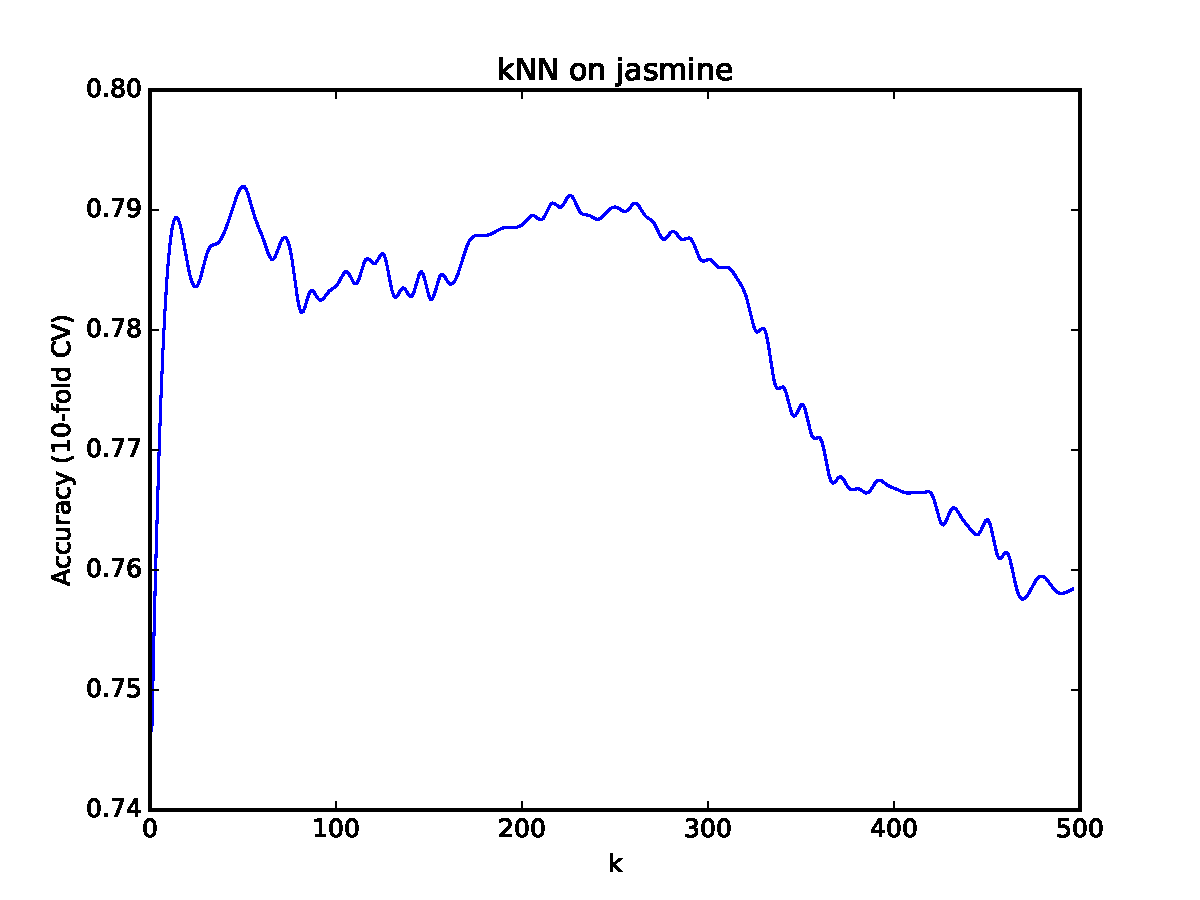
\includegraphics[width=0.6\textwidth]{images/kNN-jasmine}

\begin{itemize}
  \item $k$-nearest neighbors is one of the most trivial ML algorithms
  \item Size of neighbourhood ($k$) is very important for its performance
  \item The performance function depending on $k$ is quite complex\\ (not at all convex)
\end{itemize}

\end{frame}
%-----------------------------------------------------------------------
%----------------------------------------------------------------------
\begin{frame}[c]{Goal of AutoML}

\begin{block}{AutoML}
The goal of AutoML is to automate all parts of machine learning (as needed)
to \emph{support} users efficiently building their machine learning applications.
\end{block}

\bigskip

\begin{block}{AutoML System}
Given
\begin{itemize}
  \item a dataset
  \item a task (e.g., regression or classification)
  \item a performance metric (e.g., accuracy or RMSE)
\end{itemize}
an AutoML system automatically determines the approach 
that performs best for this particular application.
\end{block}

\end{frame}
%-----------------------------------------------------------------------
%----------------------------------------------------------------------
\begin{frame}[c]{AutoML in Research}

AutoML enables:

\begin{enumerate}
  \item more efficient research
  \begin{itemize}
    \item AutoML has shown on subproblems to outperform human experts
  \end{itemize}
  \pause
  \smallskip
  \item more systematic research
  \begin{itemize}
    \item humans tend to be unsystematic which leads to errors
  \end{itemize}
  \smallskip
  \pause
  \item more reproducible research
  \begin{itemize}
    \item since AutoML is systematic and human's unsystematic approaches cannot be reproduced 
  \end{itemize}
  \item broader use of ML also in other disciplines
  \begin{itemize}
    \item ML should not be limited to computer scientists;
    \item the most amazing applications of ML is often done\\ by either interdisciplinary teams or even non-computer scientists
  \end{itemize}
\end{enumerate}

\end{frame}
%-----------------------------------------------------------------------
%----------------------------------------------------------------------
\begin{frame}[c]{Challenges in AutoML}

\begin{enumerate}
  \item Design decisions have to be made for each dataset again
  \item Training of a single ML model can be quite expensive\\
  		(e.g., hours, days or weeks)
  \begin{itemize}
    \item[$\leadsto$] often, we cannot try a many design decisions
  \end{itemize}
  \item the mathmatical relation between design decisions\\ and performance is (often) unknown
  \begin{itemize}
    \item[$\leadsto$] gradient-based optimization is not directly possible
  \end{itemize}
  \item optimization in highly complex spaces
  \begin{itemize}
    \item incl. categorical choices, continuous parameters,\\ conditional dependencies
  \end{itemize}
  
\end{enumerate}

\end{frame}
%-----------------------------------------------------------------------
%----------------------------------------------------------------------
\begin{frame}[c]{Risks of AutoML}

What could be risks of AutoML?
\hands
\pause

\begin{enumerate}
  \item Users apply AutoML without understanding anything.
  \begin{itemize}
    \item Users might wonder why (Auto-)ML does not perform well\\ after they passed poor data. 
  \end{itemize}
  \pause
  \item The users over-trust the AutoML too much.
  \begin{itemize}
    \item humans might not use human reasoning skills and do not second guess machine decisions
  \end{itemize}
  \pause
  \item We enable non-ML experts to use ML\\ without knowing the risks and consequences of ML.
  \pause
  \item Could result in deployment of \ldots
  \begin{itemize}
    \item inaccurate ML models due to lack of understanding of statistical concepts, e.g., sampling bias, overfitting, concept drift, \ldots
    \item biased and unfair models due to lack of understanding ethical practices and use of features such as gender and race for predicting outcomes
  \end{itemize}
\end{enumerate}

See \textit{\href{https://arxiv.org/abs/1902.06804}{Democratisation of Usable Machine Learning in Computer Vision}}

\end{frame}
%-----------------------------------------------------------------------
%----------------------------------------------------------------------
\begin{frame}[c]{Snipped of Meta-Algorithmic Hierarchy}


Meta-algorithmic approaches

\begin{itemize}
  \item[$\subset$] AutoAI
  \pause
  \begin{itemize}
		\item[$\subset$] AutoML
		\pause
		\begin{itemize}
		 	\item[$\subset$] Hyperparameter optimization (HPO)
		 	\pause
		 	\item[$\subset$] Neural architecture search (NAS)\\
		 	   \hspace{1em} Google sometimes claims: AutoML $==$ NAS\\
		 	   \hspace{1em} but that's wrong!
		 	\pause
		 	\item[$\subset$] Meta-learning\\
		\end{itemize}
		\pause
		\item[$\subset$] Algorithm configuration
	\end{itemize}
	\pause
	\item[$\subset$] Search-based software engineering
\end{itemize}

\end{frame}
%-----------------------------------------------------------------------
%----------------------------------------------------------------------
\begin{frame}[c]{Goals of the Lecture}

You will be able to \ldots
\begin{enumerate}
  \item use AutoML tools
  \smallskip
  \item develop AutoML tools
  \smallskip
  \item have a good overview over the state-of-the-art in AutoML
  \smallskip
  \item do research on AutoML yourself
  \begin{itemize}
    \item perfect opportunity to do a master project or thesis with us afterwards
  \end{itemize}
\end{enumerate}

\end{frame}
%-----------------------------------------------------------------------
%----------------------------------------------------------------------
\begin{frame}[c]{Course Overview}

\begin{itemize}
	\item Introduction
	\item Background
	\begin{itemize}
		\item Design spaces in ML
		\item Experimentation and visualization
	\end{itemize}
	\item Hyperparameter optimization (HPO)
	\begin{itemize}
	  \item Bayesian optimization
	  \item Other black-box techniques
	\end{itemize}
	\item Speeding up HPO with multi-fidelity optimization
	\item Pentecost (Holiday) -- no lecture
	\item Architecture search I + II
	\item Meta-Learning
	\item Learning to learn $\&$ optimize
	\item Beyond AutoML: algorithm configuration and control
	\item Project announcement and closing
\end{itemize}


\end{frame}
%----------------------------------------------------------------------
%----------------------------------------------------------------------
\begin{frame}[c]{Course Format}

\begin{itemize}
	\item Concepts over details
	\begin{itemize}
	  \item we provide references and links to papers\\ s.t. you can read up details!
	\end{itemize}
	\smallskip
	\item Interactive lecture
	\begin{itemize}
	  \item more efficient learning through self-reflection on challenges!
	\end{itemize}
	\smallskip
	\item Practical exercises
	\begin{itemize}
	  \item implement it, use it and play with it!
	\end{itemize}
\end{itemize}

\end{frame}
%----------------------------------------------------------------------
%----------------------------------------------------------------------
\begin{frame}[c]{Team - Lectures}

\begin{columns}[T]
\column{0.3\textwidth}

\centering
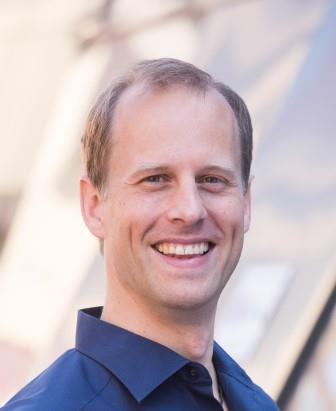
\includegraphics[width=9em]{images/team/frank_small}

Prof. Dr. Frank Hutter

\column{0.3\textwidth}
\centering
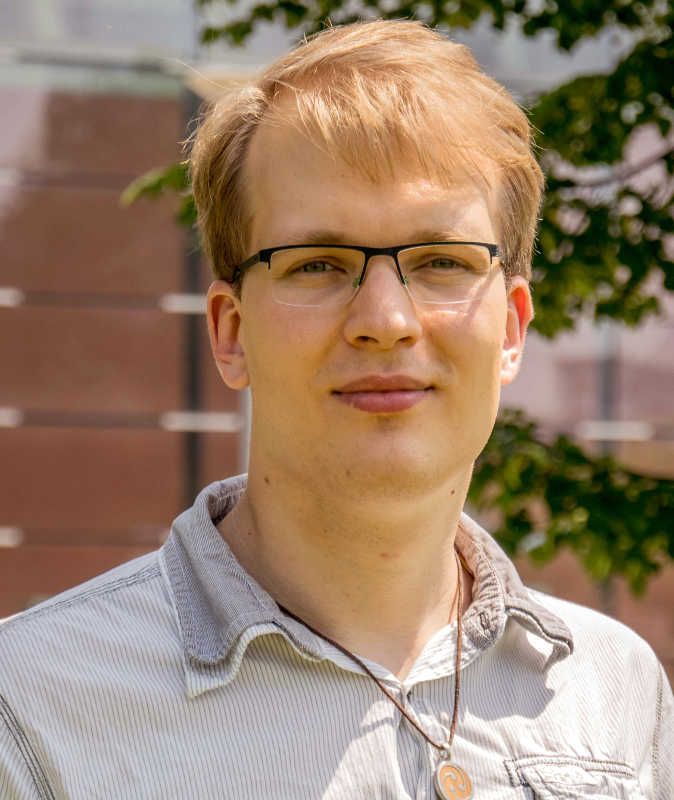
\includegraphics[width=9em]{images/team/marius}

Dr. Marius Lindauer

\column{0.3\textwidth}
\centering

\includegraphics[width=9em]{images/team/awad_small}

Dr. Noor Awad\\
(guest lecturer)


\end{columns}

\end{frame}
%----------------------------------------------------------------------
%----------------------------------------------------------------------
\begin{frame}[c]{Team -- Exercise}

\begin{columns}[T]

\column{0.3\textwidth}
\centering
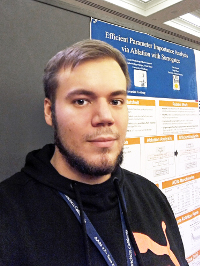
\includegraphics[height=9em]{images/team/biedenkapp}
André Biedenkapp
\column{0.3\textwidth}
\centering
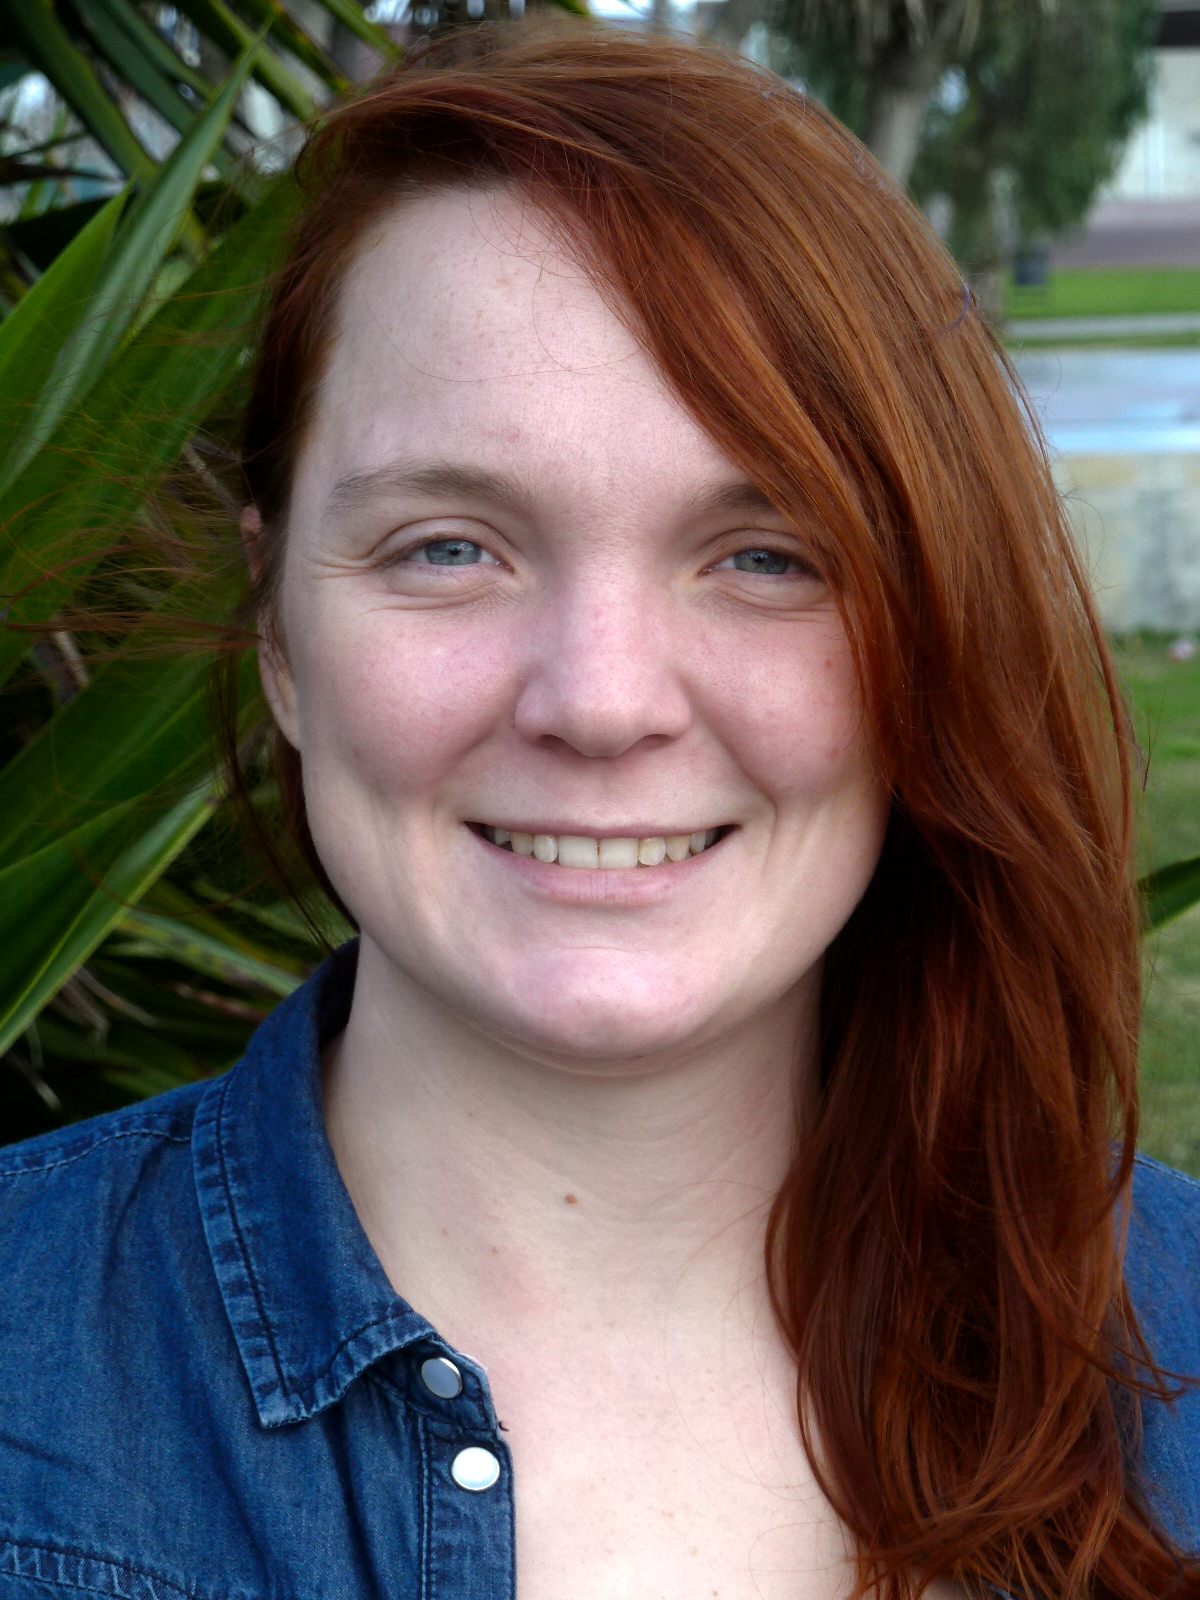
\includegraphics[height=9em]{images/team/eggensperger_small}
Katharina Eggensperger
\column{0.3\textwidth}
\centering
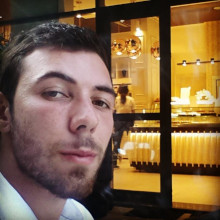
\includegraphics[height=9em]{images/team/arber_small}
Arber Zela

\end{columns}

\end{frame}
%----------------------------------------------------------------------
%----------------------------------------------------------------------
\begin{frame}[c]{Organization (Lectures)}

\begin{itemize}
  \item $6$ ECTS
  \item Every week at Monday: 14:15 (s.t) - 15:45\\ (Building: 106 Room: SR 00 007)
  \item \emph{Interactive} Lecture 
  \begin{itemize}
    \item We will ask you questions in the lectures
    \item Kahoot quiz at the end of each lecture
  \end{itemize}
  \item Course material on our homepage\\
  		{\small \url{ml.informatik.uni-freiburg.de/teaching/ss2019/automl/}}
  \item Slides will be online before the lectures
  \item No video recording!
\end{itemize}

\end{frame}
%-----------------------------------------------------------------------
%----------------------------------------------------------------------
\begin{frame}[c]{Organization (Exercises)}

\begin{itemize}
  \item Every Friday at: 14:15 - 15:45\\ (Building: 106 Room: SR 00 007)
  \begin{itemize}
    \item No meeting this week, but first exercise sheet!
  \end{itemize}
  \item Every week new exercise sheet and discussion of last exercise
  \item Most exercises will be practical, i.e., you have to implement something
  \item Team work allowed, max team size: 2! 
  \item Cheating:
  \begin{itemize}
    \item First time cheating: $0$ points for exercise
    \item Second time cheating: failing the course
  \end{itemize}
  \item You have to obtain at least $50\%$ points in the exercises  
  \item The number of points per sheet will slightly increase over time
  \item Submit via bitbucket (git)
\end{itemize}

\end{frame}
%-----------------------------------------------------------------------
%----------------------------------------------------------------------
% \begin{frame}[c]{Exceptions (tentative)}
% 
% \begin{itemize}
% 	\item No lectures and exercises during vacations and holidays\\ (1. Nov, 25. Dec, 27. Dec, 01. Jan, 03. Jan)
% 	\item Switching lecture and exercise slot 11. Dec and 13. Dec
% 	\item Last lecture at 05. Feb
% \end{itemize}
% 
% \end{frame}
%-----------------------------------------------------------------------
%----------------------------------------------------------------------
\begin{frame}[c]{Requirements}

\begin{itemize}
  \item Knowledge in \alert{Machine Learning} (strongly recommended)
  \begin{itemize}
    \item Classification, regression, clustering, decision tree, training-test split, cross validation, pre-processing \ldots
  \end{itemize}
  \pause
  \item Knowledge in \alert{Deep Learning} (strongly recommended)
  \begin{itemize}
    \item feed-forward network, recurrent network, convolutions, learning rates, regularization, \ldots 
  \end{itemize}
  \pause
  \item Experience in \alert{Python and git} (recommended)
  \begin{itemize}
    \item nearly all exercises will require 
    that you implement something in~Python and submit the solution to a git repo
  \end{itemize}
\end{itemize}

\end{frame}
%-----------------------------------------------------------------------
%----------------------------------------------------------------------
\begin{frame}[c]{Final Oral Exam}

\begin{itemize}
  \item Implement a larger project (worth $1-2$ weeks fulltime)
	\begin{itemize}
		\item No teamwork!
	\end{itemize}
  \item Exam
	\begin{itemize}
		\item Present the project in the first $15$ minutes\\ (including some questions from us)
		\item Answer questions about further course material in the second $15$ minutes
	\end{itemize}	
  \item tentative date: end of September
\end{itemize}

\end{frame}
%----------------------------------------------------------------------
%----------------------------------------------------------------------
\begin{frame}[c]{Resources}

\begin{itemize}
  \item To get a deep understanding of AutoML, you should also read some literature 
  \item We will provide links to papers at the end of each lecture
  \item New AutoML book: \url{https://www.automl.org/book/}
  \begin{itemize}
    \item Draft online available
  \end{itemize}
\end{itemize}

\end{frame}
%----------------------------------------------------------------------
%----------------------------------------------------------------------
\begin{frame}[c]{Chances and Risks}

AutoML is an advanced lecture and we modify it each time.

\bigskip
\pause

Chances:
\begin{itemize}
  \item All presented topics are close to state-of-the-art;\\there is active research on these topics  
  \item The course will provide a solid background\\ for doing a master project/thesis in our group 
\end{itemize}

\medskip

Risks:
\begin{itemize}
  \item You will find some typos and issues in the slides;\\ please tell us if you find something
  %\item Workload could be very high for you -- we have no experience with the exercises yet
\end{itemize}

\medskip
\pause
$\to$ Give us some feedback and we will improve the course!

\medskip
\pause
Note: AutoML was already partially covered in our old lecture ML4AAD. 
If you successfully attended ML4AAD, please don't attend AutoML.

\end{frame}
%-----------------------------------------------------------------------
%----------------------------------------------------------------------
\begin{frame}[c]{Introduce yourself!}

\begin{itemize}
  \item Why have you chosen this course?
  \medskip
  \item Background knowledge? (ML, DL, \ldots)
  \medskip 
  \item Experience with such problems?
\end{itemize}

\bigskip
\centering
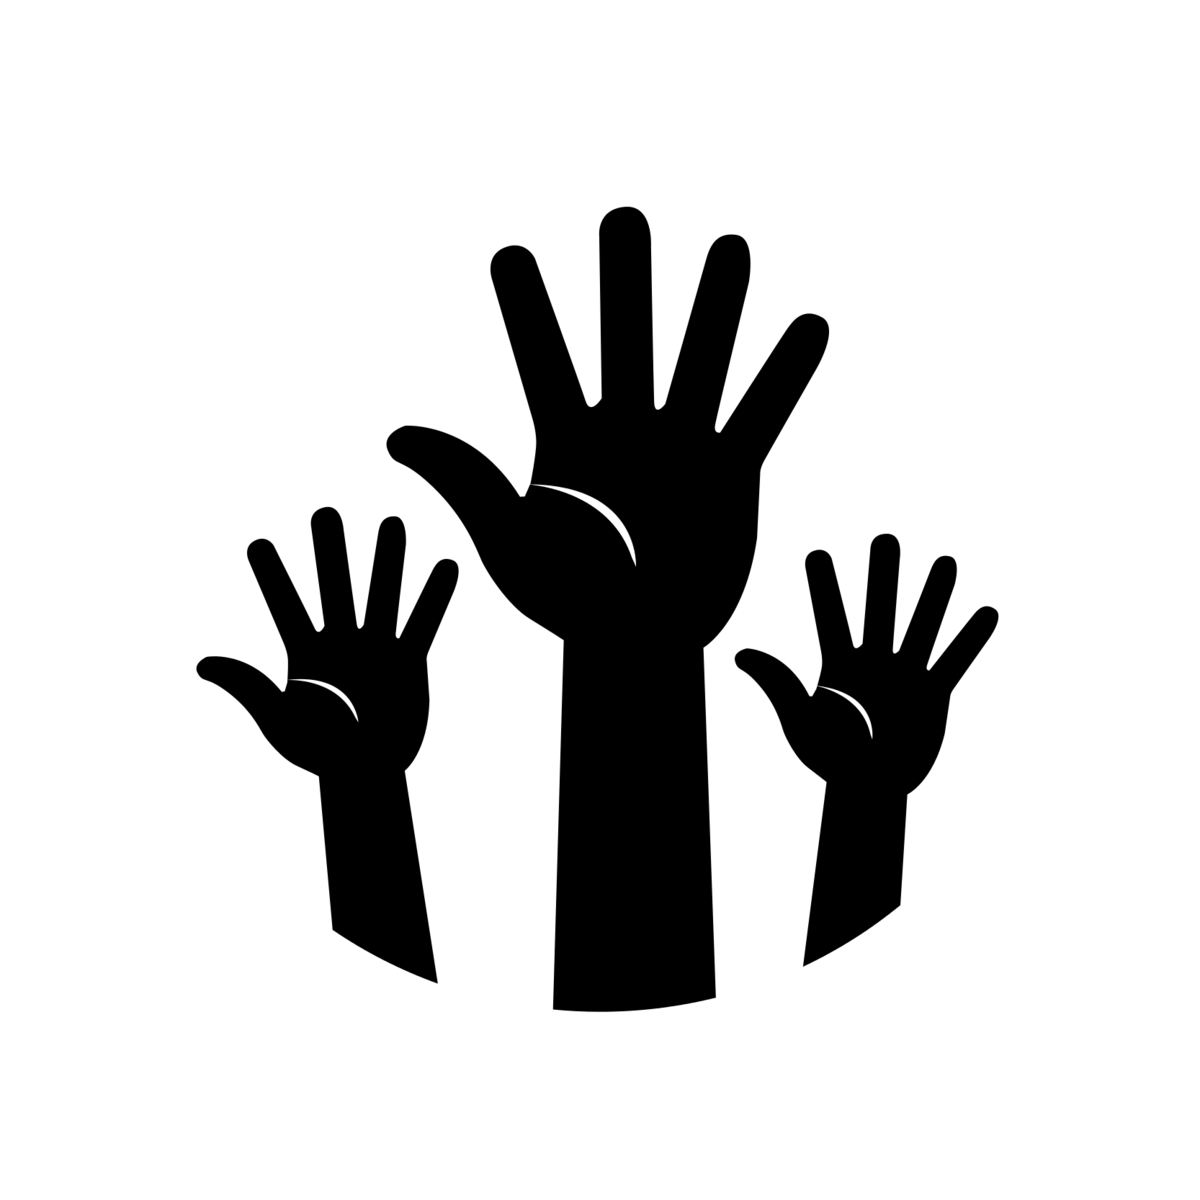
\includegraphics[scale=0.1]{images/hands.png}

\end{frame}
%-----------------------------------------------------------------------
%----------------------------------------------------------------------
% \begin{frame}[c]{Exercise I }
% 
% \begin{block}{Task}
% \begin{enumerate}
% 	\item Identify $2$ (known) algorithms which have tunable parameters and briefly describe these parameters
% 	\item Describe a manual way to tune the parameters and approximate the effort you would need to do this on an example
% 	\item Analyze the runtime complexity of the algorithms
% \end{enumerate}
% \end{block}
% 
% \alert{Submission due 02.11. (23:59 GMT)}\\
% Submit at ILIAS : \url{https://ilias.uni-freiburg.de/goto.php?target=crs_465155&client_id=unifreiburg}
% %Send to: \url{lindauer@cs.uni-freiburg.de}\\
% %with subject: \texttt{[MLOAD Excercise I] $<$your name$>$} 
% 
% \end{frame}
%-----------------------------------------------------------------------
% %----------------------------------------------------------------------
% \begin{frame}[c]{}
% 
% 
% 
% \end{frame}
% %-----------------------------------------------------------------------


%\begin{frame}[c]{}

\centering
\huge
Lecture 2:\\
Design Spaces in Machine Learning
\end{frame}
%----------------------------------------------------------------------
%----------------------------------------------------------------------
\begin{frame}[c]{Where are we? The big picture}

\begin{itemize}
	\item Introduction
	\item[$\to$] Background
	\begin{itemize}
		\item[$\to$] Design spaces in ML
		\item Experimentation and visualization
	\end{itemize}
	\item Hyperparameter optimization (HPO)
	\begin{itemize}
	  \item Bayesian optimization
	  \item Other black-box techniques
	\end{itemize}
	\item Speeding up HPO with multi-fidelity optimization
	\item Pentecost (Holiday) -- no lecture
	\item Architecture search I + II
	\item Meta-Learning
	\item Learning to learn $\&$ optimize
	\item Beyond AutoML: algorithm configuration and control
	\item Project announcement and closing
\end{itemize}


\end{frame}
%----------------------------------------------------------------------
%----------------------------------------------------------------------
\begin{frame}[c]{Learning Goals}

After this lecture, you will be able to \ldots

\begin{itemize}
  \item identify design decisions of machine learning algorithms
  \item explain different types of design decisions and there relations
  \item create design spaces
  \item discuss the pros and cons of different design space approaches
  \item explain design spaces for neural architecture search
\end{itemize}

\end{frame}
%----------------------------------------------------------------------
%----------------------------------------------------------------------
\begin{frame}[c]{Simple Design Decisions: Selection of Algorithm}

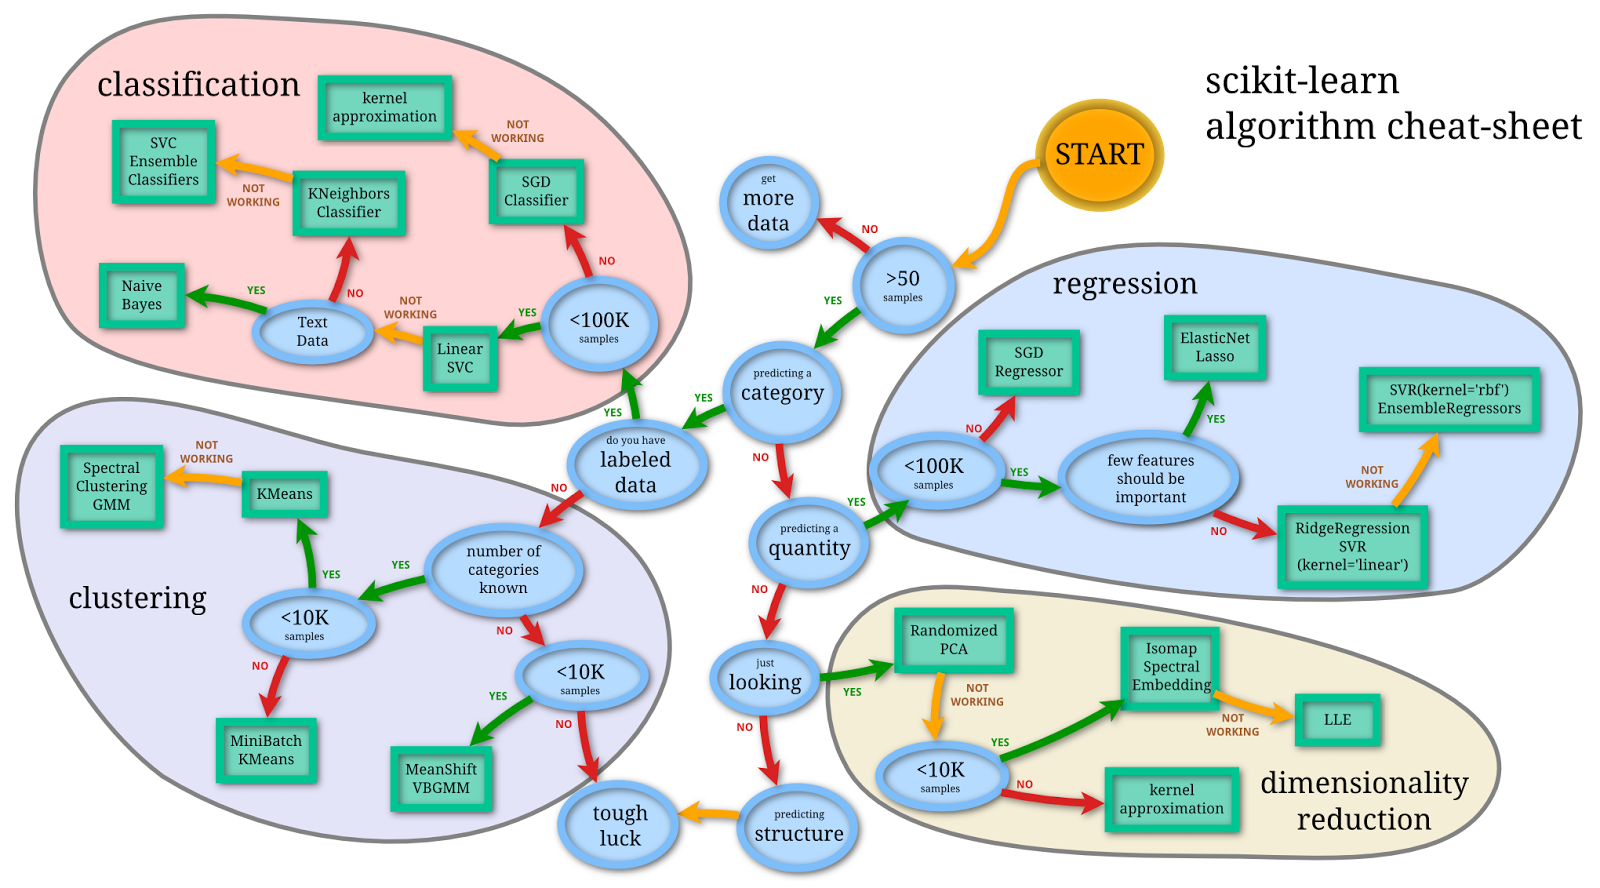
\includegraphics[width=1.0\textwidth]{images/sklearn-cheat}


\end{frame}
%----------------------------------------------------------------------
%----------------------------------------------------------------------
\begin{frame}[c]{Simple Design Decisions: Selection of Algorithm}

\begin{itemize}
  \item categorical design decison: $\{ \algo_1, \algo_2, \algo_3, \ldots, \algo_n\}$
  \begin{itemize}
	\item random forest (RF), support vector machine (SVM),\\ gradient boosting (GB), \ldots
    \item there is no ordering between algorithms
    \item set notation
  \end{itemize}
  \pause
  \item if we would run all of them and each takes (on average) $t$ seconds:\\
  $t \cdot n$ seconds
  \pause
  \smallskip
  \item in addition, choose pre-processing algorithm: $\{\algo_1^P, \algo_2^P, \algo_3^P, \ldots \algo_l^P \}$
  \begin{itemize}
    \item PCA, feature selection, random kitchen sinks, \ldots
  \end{itemize}
  \item if we only use one preprocessor and one ML algorithm,\\ brute force would require:
  $t \cdot n \cdot l$
\end{itemize}

\end{frame}
%----------------------------------------------------------------------
\section{Design Space from Documentation}
%----------------------------------------------------------------------
\begin{frame}[c]{Design Space of Support Vector Machines}

\centering
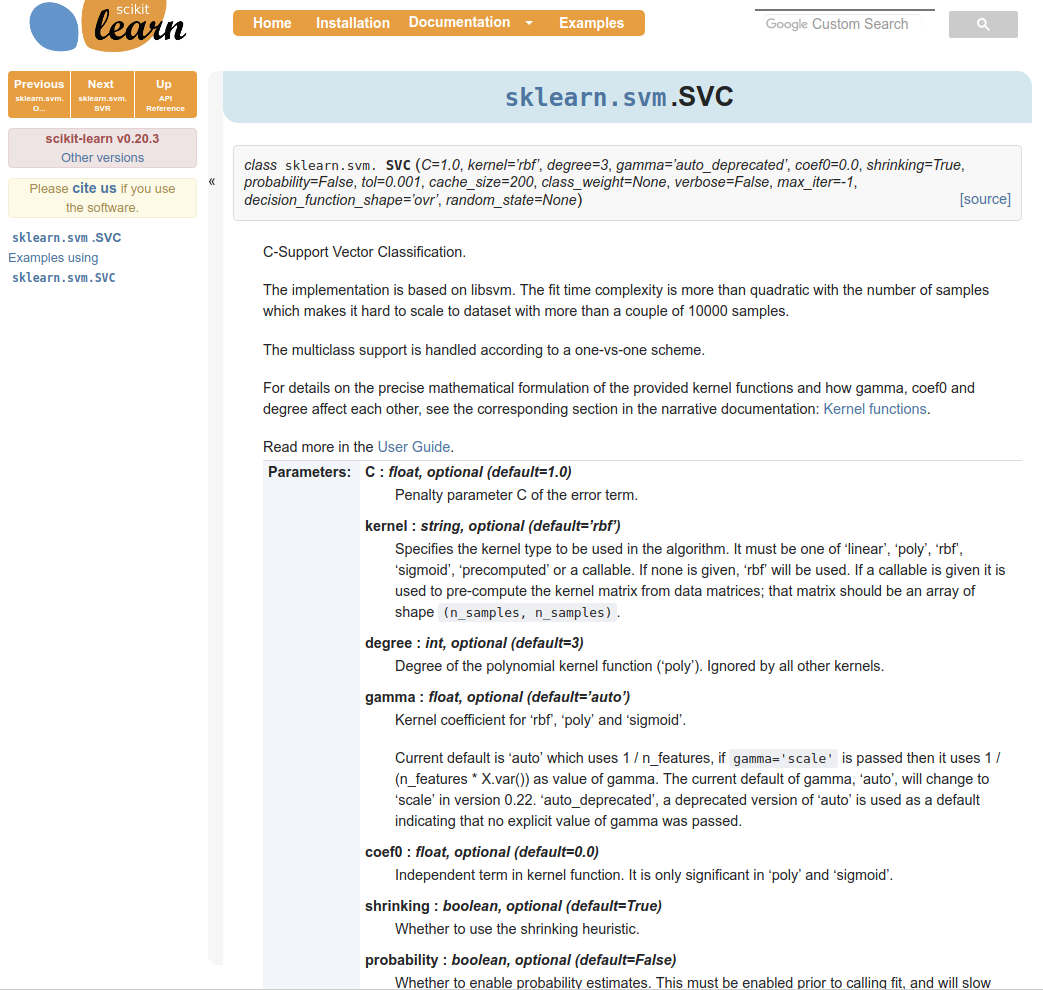
\includegraphics[width=0.7\textwidth]{images/sklearn_svm_doc.png}

\end{frame}
%----------------------------------------------------------------------
%----------------------------------------------------------------------
\begin{frame}[c]{Design Space of Support Vector Machines}

\begin{block}{Hyperparameter Optimization (HPO; informal)}
Given
\begin{itemize}
  \item a dataset
  \item a set of hyperparameters of a machine learning algorithms
  \item a cost metric (e.g., predictive error)
\end{itemize}
we want to find the hyperparameter configuration\\ that minimizes the cost metric wrt the dataset. 
\end{block}

\begin{block}{Hyperparameter Types of SVM}
\begin{description}
  \item[C] float hyperparameter
  \item[Kernel] categorical hyperparameter
  \item[Degree] integer hyperparamerter
  \item[gamma] float hyperparamerter
  \item \ldots
\end{description}
\end{block}

\end{frame}
%----------------------------------------------------------------------
%----------------------------------------------------------------------
\begin{frame}[c]{Hyperparameter Types}

\begin{description}
	\item[categorical] set of values (not sorted, no distance)
	\begin{itemize}
	  \item \texttt{kernel \{linear, rbf, poly, sigmoid\}}
	\end{itemize}
	\pause
	\item[ordinal] list of ordered values with uniform distance
	\begin{itemize}
	  \item no example in SVM design space
	  \item \texttt{size [small, medium, large]}
	\end{itemize}
	\pause
	\item[integer] bounded range of integers
	\begin{itemize}
	  \item \texttt{degree [1, 5]}
	\end{itemize}
	\pause
	\item[float] bounded range of floats
	\begin{itemize}
	  \item \texttt{gamma\_value [0.0001, 8.0]}
	\end{itemize}
\end{description}

\end{frame}
%----------------------------------------------------------------------
%----------------------------------------------------------------------
\begin{frame}[c,fragile]{Design Space and Configuration}

\begin{block}{Design/Configuration Space}
The combination of several hyperparameter ranges $\pcs_i$ for the $i$-th hyperparameter creates a design space:
$\pcs = \pcs_1 \times \pcs_2 \times \pcs_3 \ldots \times \pcs_n$ 

\pause
\bigskip

For example, the design space of a SVM would include:

\begin{verbatim}
kernel categorical {linear, rbf, poly, sigmoid}
degree integer [1, 5]
gamma_value float [0.0001, 8.0]
\end{verbatim}
\end{block}

\pause

\begin{block}{Configuration}
An element of the configuration space $\conf \in \pcs$ instantiates each hyperparameter $\conf_i$ with a value.
For example:
\begin{verbatim}
{kernel: rbf, gamma_value: 1, degree: 2}
\end{verbatim}

\end{block}

\end{frame}
%----------------------------------------------------------------------
%----------------------------------------------------------------------
\begin{frame}[c]{Concept of Defaults}

\begin{itemize}
  \item We assume that each algorithm has a default
  \begin{itemize}
    \item often a robust configuration if you don't want to change it
    \item defaults often provided by developer, e.g.,\\
   		  in its documentation or the corresponding paper
  \end{itemize}
  \pause
  \item We use the default to start our search for HPO
  \begin{itemize}
    \item if we know a reasonable configuration,\\ we should start with a random configuration?
    \item Goal: find something which is better than the default
    \pause
    \smallskip
    \item Pro: Can help us to start in good region of the design space
    \item Contra: We might start being trapped in local optimum.
  \end{itemize}
\end{itemize}

\pause
Example: the default \texttt{kernel} of the SVM could be the RBF-kernel\\
\texttt{kernel categorical \{linear, rbf, poly, sigmoid\}[rbf]}

\end{frame}
%----------------------------------------------------------------------
%----------------------------------------------------------------------
\begin{frame}[c, fragile]{Conditional Dependencies}

\begin{block}{SVM Example}
\begin{verbatim}
kernel categorical {linear, rbf, poly, sigmoid}[rbf]
degree integer [1, 5][3]
gamma_value float [0.0001, 8.0][2.0]
\end{verbatim}
\end{block}

\begin{itemize}
  \item Some parameters depend on each other
  \begin{itemize}
    \item \texttt{degree} is only active if \texttt{kernel} is set to \texttt{poly}
    \item \texttt{gamma\_value} is only active if \texttt{kernel} is set to \texttt{rbf}  
  \end{itemize}
  \bigskip
  \pause
  \item[$\leadsto$] model such conditional dependencies in configuration space:
\end{itemize}

\begin{verbatim}
degree | kernel in {poly}
gamma_value | kernel in {rbf}
\end{verbatim}

\end{frame}
%----------------------------------------------------------------------
%----------------------------------------------------------------------
\begin{frame}[c, fragile]{Remarks (I): Conditional Dependencies}

\begin{block}{Duplicates of Hyperparameters?}
\begin{itemize}
	\item Sometimes algorithms have the same sub-hyperparameter\\ (with slightly different meanings)
	\item Two approaches:
	\begin{itemize}
		\item Duplicate hyperparameter and use conditionals \\
		$\leadsto$ larger configuration space
		\item a single hyperparameter\\
		$\leadsto$ optimizer has to learn dependencies on its own
	\end{itemize}
    \item Not well studied which of the two ways is better under which conditions
\end{itemize}
\end{block}
	
\end{frame}
%----------------------------------------------------------------------
%----------------------------------------------------------------------
\begin{frame}[c, fragile]{Remarks (II): Conditional Dependencies}

\begin{block}{Imputation}
	\begin{itemize}
		\item Inactive hyperparameters can be handled in different ways
		\item Most trivial approach: imputation of deactivated hyperparameters
		\begin{enumerate}
			\item Impute with default value
			\item Impute with non-existing value
		\end{enumerate}
		\pause
		\medskip
		\item Risk:
		\begin{itemize}
			\item confusing for some optimizers (in particular model-based optimizers)
		\end{itemize}
		\pause
		\item One of the open challenges: best way to handle conditionals
	\end{itemize}
\end{block}

\end{frame}
%----------------------------------------------------------------------
%----------------------------------------------------------------------
\begin{frame}[c, fragile]{Forbidden Constraints}

\begin{itemize}
  \item sometimes combinations of settings are forbidden
  \item For example: $a \leq b$
  \smallskip
  \pause
  \item[$\leadsto$] Try to avoid such constraints\\ because sampling in constrained spaces gets much harder
  \smallskip
  \item Sometimes constraints can be rewritten:
\end{itemize}

\begin{verbatim}
    a float [0,1][0]
    b float [0,1][0]
    a <= b
\end{verbatim}

Rewrite:
\begin{verbatim}
    a float [0,1][0]
    c float [0,1][0]
\end{verbatim}

with $b = a + c$ $\leadsto$ \texttt{b} might be larger than 1! 


\end{frame}
%----------------------------------------------------------------------
%----------------------------------------------------------------------
\begin{frame}[c, fragile]{Expert Knowledge: Transformations}

\begin{itemize}
	\item Expert knowledge can help to guide hyperparameter optimization
	\item For example, some hyperparameters might not be sampled uniformly
\end{itemize}

\pause
\medskip
For example, regularization hyperparameter of SVM:

\begin{verbatim}
    C float [0.001, 1000.0][1.0]
\end{verbatim}

\begin{itemize}
	\item the distance between $999.9$ and $1000.0$ should not be the same as between $0.001$ and $0.101$
	\smallskip
	\pause
	\item[$\leadsto$] We might want to sample here from from a log-scale
\end{itemize}

\begin{verbatim}
    C float [0.001, 1000.0][1.0] log
\end{verbatim}

\end{frame}
%----------------------------------------------------------------------
%----------------------------------------------------------------------
\begin{frame}[c]{Design Space of Support Vector Machines}

\centering
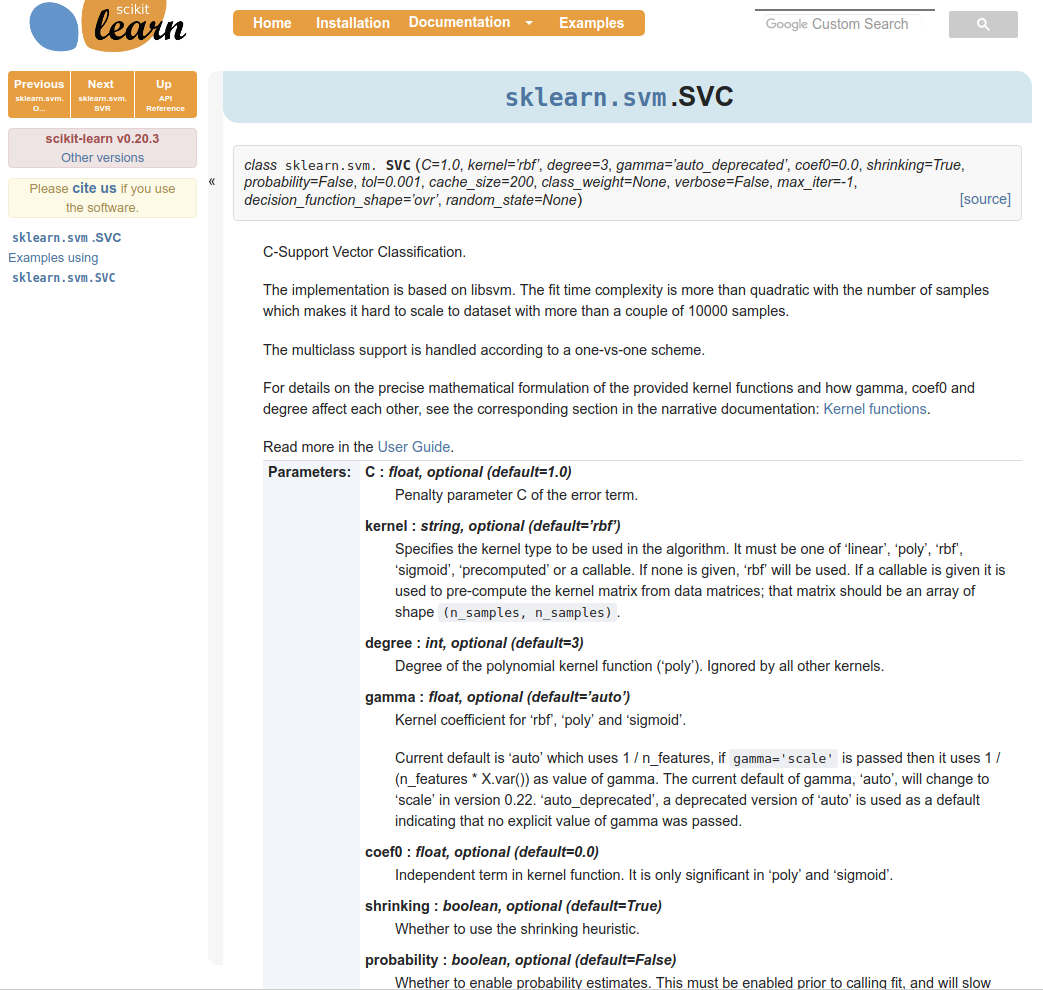
\includegraphics[width=0.7\textwidth]{images/sklearn_svm_doc.png}

\end{frame}
%----------------------------------------------------------------------
%----------------------------------------------------------------------
\begin{frame}[c, fragile]{Configuration Space of SVM}

\begin{verbatim}
  Hyperparameters:
    C float [0.001, 1000.0][1.0] log
    coef0 float [0.0, 10.0][0.0]
    degree integer [1, 5][3]
    gamma categorical {auto, value}[auto]
    gamma_value float [0.0001, 8.0][1.0]
    kernel categorical {linear, rbf, poly, sigmoid}[poly]
    shrinking categorical {true, false}[true]
  Conditions:
    coef0 | kernel in {poly, sigmoid}
    degree | kernel in {poly}
    gamma | kernel in {rbf, poly, sigmoid}
    gamma_value | gamma in {value}
\end{verbatim}

\end{frame}
%----------------------------------------------------------------------
%----------------------------------------------------------------------
\begin{frame}[c, fragile]{Optimization of Random Seeds?}

Is the random seed a valid design decision?

\medskip

\begin{block}{Output: trained model}
	If the output of your AutoML tool is a trained model:
	\begin{itemize}
		\item your goal is to obtain the best trained model
		\item[$\leadsto$] tune your random seed!
	\end{itemize}
\end{block}

\pause	
\medskip
	
\begin{block}{Output: best configuration}
	If the output of your AutoML tool is the best configuration:
	\begin{itemize}
		\item your goal is to obtain a configuration that performs well after refitting 
		\item[$\leadsto$] don't tune your random seed!
		\item[$\leadsto$] obtain configuration that performs well on many random seeds
	\end{itemize}
\end{block}


\end{frame}
%----------------------------------------------------------------------
\section{Design Space from Algorithm}
%----------------------------------------------------------------------
\begin{frame}[c]{Algorithm: Randomized Regression Tree}

\begin{algorithm}[H]
\Input{$D = \{(\vec{x}^{(i)}, y^{(i)})\}_{i\in \{1\ldots|D|\}}$, attributes A}
\BlankLine
\If{current tree depth larger than threshold $t_d$} {
	  \Return{Leaf with $\vec{y}$}
}
\If{samples size $|D|$ is smaller than threshold $t_n$} {
	  \Return{Leaf with $\vec{y}$}
}
\pause
$A'$ $\leftarrow$ subsample $k$ attributes from $A$;\\
let $v$ be the \emph{best split value} of attribute $a \in A'$ according to criterion $c$;\\ 
\pause
Create edges with constraint $\vec{x}^{(i)}.a \leq v$ and $\vec{x}^{(i)}.a > v$;\\
BuildTree($\{ (\vec{x}^{(i)}, y^{(i)}) \in D | \vec{x}^{(i)}.a \leq v\}$, $A$);\\
BuildTree($\{ (\vec{x}^{(i)}, y^{(i)}) \in D | \vec{x}^{(i)}.a > v\}$, $A$);
	
\Return{current node}
\caption{\texttt{BuildTree()}}
\end{algorithm}

\end{frame}
%----------------------------------------------------------------------
%----------------------------------------------------------------------
\begin{frame}[c]{Algorithm: Regression Random Forest}

\begin{algorithm}[H]
\Input{$D = \{(\vec{x}^{(i)}, y^{(i)})\}_{i\in \{1\ldots|D|\}}$, attributes A}
\BlankLine

\For{$i \in \{1 \ldots n\}$}{
	$D'$ $\leftarrow$ bootstrap $D$ with $d$ points;\\
	$T_i$ $\leftarrow$ BuildTree($D'$, $A$);\\
}
	
\caption{\texttt{BuildForest()}}
\end{algorithm}

\pause
\bigskip

\begin{algorithm}[H]
\Input{Data point $x$}
\BlankLine

\For{$i \in \{1 \ldots n\}$}{
        $y_i$ $\leftarrow$ $T_i$.predict($x$); \\
}

$y$ $\leftarrow$ $\frac{1}{n}\sum_{i}^n y_i$;\\
	
\caption{\texttt{Predict()}}
\end{algorithm}


\end{frame}
%----------------------------------------------------------------------
\begin{frame}{Configuration Space of Regression Random Forest}

Task: \hands [5min]
\begin{itemize}
  \item What are design decisions of a regression random forest?
  \item What could be a reasonable configuration space?  
\end{itemize}

\end{frame}
%----------------------------------------------------------------------
%----------------------------------------------------------------------
\begin{frame}[c]{Levels of Programming by Optimization \litw{Hoos 2012}}

\begin{description}
\item[Level 0] Already exposed hyperparameters
\pause
\item[Level 1] Make hardwired design choices accessible
\pause
\item[Level 2] Design choices are already considered\\ during software development
\pause 
\item[Level 3] Seek design choices in software development
\end{description}

\pause
\bigskip

$\leadsto$ The field of search-based software engineering is\\ closely related to AutoML.

\end{frame}
%----------------------------------------------------------------------
\section{Hyperparameter Optimization and CASH}
%----------------------------------------------------------------------
\begin{frame}[c]{Hyperparameter Optimization}

\begin{block}{Hyperparameter Optimization (HPO)}
Given
\begin{itemize}
  \item a dataset $\dataset$
  \item a set of hyperparameters $\pcs$ of a machine learning algorithms $\algo$
  \item a cost metric or loss function $\loss$ (e.g., predictive error)
\end{itemize}
we want to find a hyperparameter configuration $\conf \in \pcs$ that minimizes $\loss$ wrt $\dataset$:

\begin{equation}
\conf^* \in \argmin_{\conf \in \pcs} \loss(\algo(\conf), \dataset) \nonumber
\end{equation}

\end{block}

\pause
Remarks: 

\begin{itemize}
  \item We use an simplified notation of the loss function $\loss$ to focus on the main point here;
  \pause
  \item $\argmin$ returns a set of optimal points of a given function. We are happy to find one element of this set and thus use $\in$ instead of $=$.
\end{itemize}

\end{frame}
%----------------------------------------------------------------------
%----------------------------------------------------------------------
\begin{frame}[c]{Extend HPO}

AutoML includes

\begin{itemize}
  \item Hyperparameter Optimization (HPO)
  \item Algorithm selection 
  \item \ldots (and more)
\end{itemize}

\pause
\bigskip
$\leadsto$ How to select an algorithm?


\end{frame}
%----------------------------------------------------------------------
%----------------------------------------------------------------------
\begin{frame}[c]{CASH \litw{Thornton et al. 2013}}

\begin{block}{CASH: Combined Algorithm Selection and Hyperparameter Optimization}
Given
\begin{itemize}
  \item a dataset $\dataset$
  \item a set of algorithms $\mathbf{A} = \{\algo_1, \algo_2, \ldots, \algo_k\}$
  \item a set of hyperparameters $\pcs$ of each machine learning algorithms $\algo_i$
  \item a cost metric or loss function $\loss$ (e.g., predictive error)
\end{itemize}
we want to find the best combination of algorithm $\algo \in \mathbf{A}$ and its hyperparameter configuration $\conf \in \pcs$ minimizing $\loss$ wrt $\dataset$:

\begin{equation}
(\algo^*, \conf^*) \in \argmin_{\algo \in \mathbf{A}, \conf \in \pcs} \loss(\algo(\conf), \dataset) \nonumber
\end{equation}

\end{block}

\end{frame}
%----------------------------------------------------------------------
%----------------------------------------------------------------------
\begin{frame}[c, fragile]{Representation of CASH}

\begin{itemize}
  \item top-level hyperparameter to select algorithm
  \item conditional constraints for all algorithm-specific hyperparameters
\end{itemize}

\pause

\begin{verbatim}
algo categorical {SVM, RF, DNN}[RF]

n_tree integer [10,100][10]
n_tree | algo in {RF}

gamma float {0.0001,8}[1]
gamma | algo in {SVM]

...
\end{verbatim}

\end{frame}
%----------------------------------------------------------------------
%----------------------------------------------------------------------
\begin{frame}[c, fragile]{Representation of CASH}

\centering
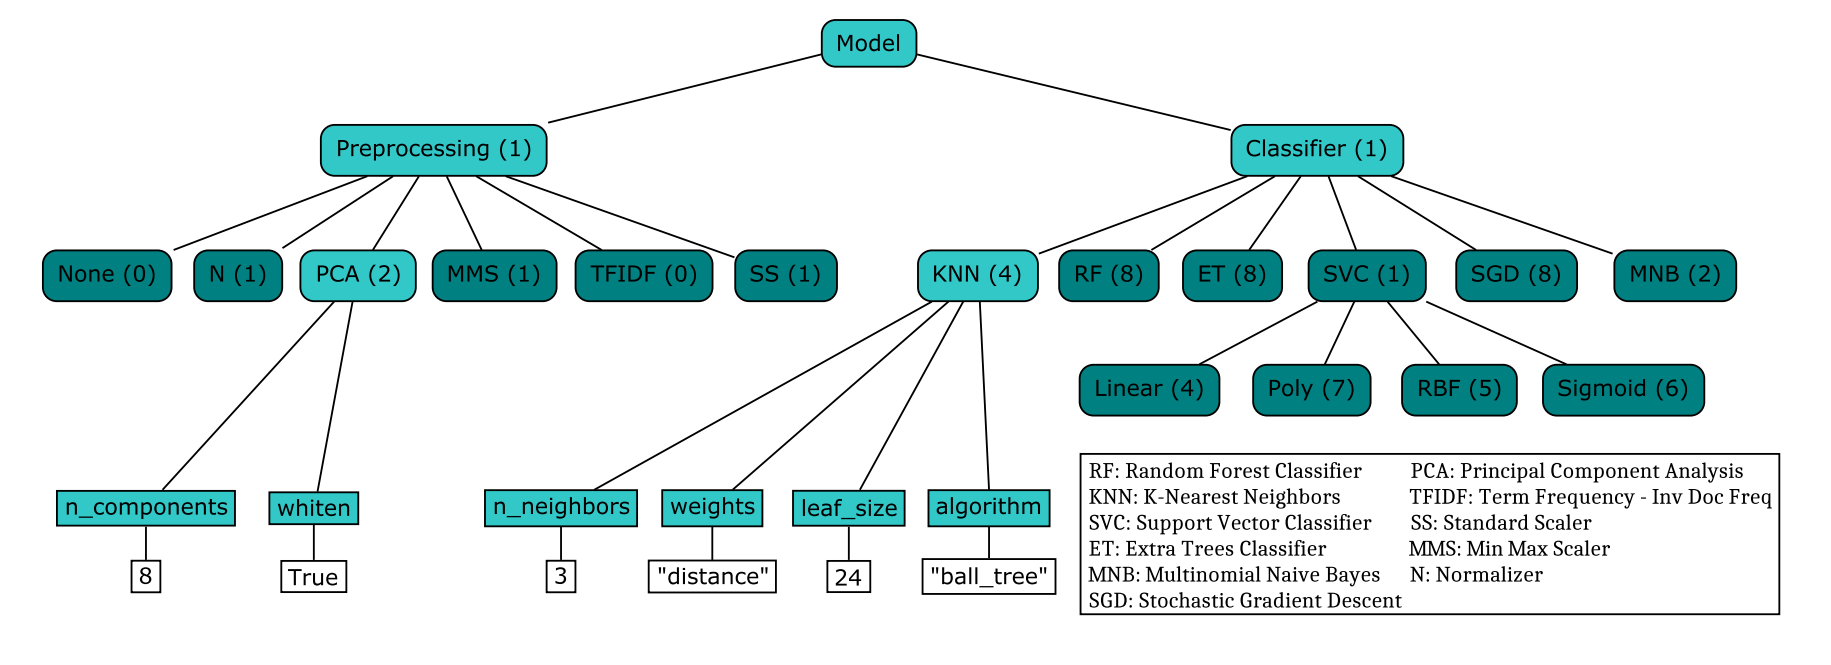
\includegraphics[width=1.0\textwidth]{images/cash}

\hfill Source: \lit{Komer et al. 2019}

\end{frame}
%----------------------------------------------------------------------

%----------------------------------------------------------------------
\begin{frame}[c, fragile]{Select several Algorithms}

We can use set of algorithms:
\begin{itemize}
  \item for example, we want to apply a set of preprocessors
  \item Each algorithm gets a binary hyperparameter
  \begin{itemize}
  	\item $2^n$ possible combinations for $n$ preprocessors	
  \end{itemize}
\end{itemize}

\begin{verbatim}
normalize categorical {True, False}[False]
pca categorical {True, False}[False]
pca_dim integer [1,100][10]
pca_dim | pca in {True}
\end{verbatim}

\end{frame}
%----------------------------------------------------------------------
\section{Unbounded Configuration Spaces}
%----------------------------------------------------------------------
\begin{frame}[c]{Bounded Configuration Spaces}

So far, we assumed that each hyperparameter has a pre-defined domain.

\medskip
Problems:
\begin{itemize}
  \item for pipelines, we might don't know the size of the pipeline
	\begin{itemize}
		\item some components could be part of the pipeline multiple times
	\end{itemize}
  \pause
  \medskip
  \item sometimes we don't know a good range for a hyperparameter
  \begin{itemize}
     \item too large range $\leadsto$ very hard optimization problem
     \item too small range $\leadsto$ we might miss high-performance areas
  \end{itemize}

\end{itemize}

\pause
\bigskip

$\leadsto$ How can we design such configuration spaces?

\end{frame}
%----------------------------------------------------------------------
%----------------------------------------------------------------------
\begin{frame}[c, fragile]{Pipeline: Boolean Options}


\begin{verbatim}
  component_1 categorical {True, False}[True]
  component_2 categorical {True, False}[False]
  component_3 categorical {True, False}[False]
  ...
\end{verbatim}

\begin{itemize}
	\item Hard to optimize if 
	\begin{itemize}
		\item we also have to find the ordering of the components
		\item if there is an upper bound on the number of components\\
		$\leadsto$ leads to many invalid configurations
		\item Each component can only be chosen once
	\end{itemize}
\end{itemize}

\end{frame}
%----------------------------------------------------------------------
%----------------------------------------------------------------------
\begin{frame}[c, fragile]{Pipeline: Fixed Pipelines Size}


\begin{verbatim}
step_1 categorical {comp1, comp2, comp3, ..., none}[comp1]
step_2 categorical {comp1, comp2, comp3, ..., none}[comp2]
step_3 categorical {comp1, comp2, comp3, ..., none}[none]
...
\end{verbatim}

\begin{itemize}
	\item encode each step of the pipeline with a choice of all possible components
	\item Hard to optimize if
	\begin{itemize}
		\item we don't know a good upper bound of the pipeline size
		\item there is an upper bound on how often a component can be chosen
	\end{itemize}
    \pause
    \bigskip
	\item If we don't need to specify the maximum length of the pipeline\\ this design is equivalent to search in a tree of possible pipelines
\end{itemize}

\end{frame}
%----------------------------------------------------------------------
%----------------------------------------------------------------------
\begin{frame}[c]{Pipeline: TPOT \litw{Olson et al. 2016}}

\centering
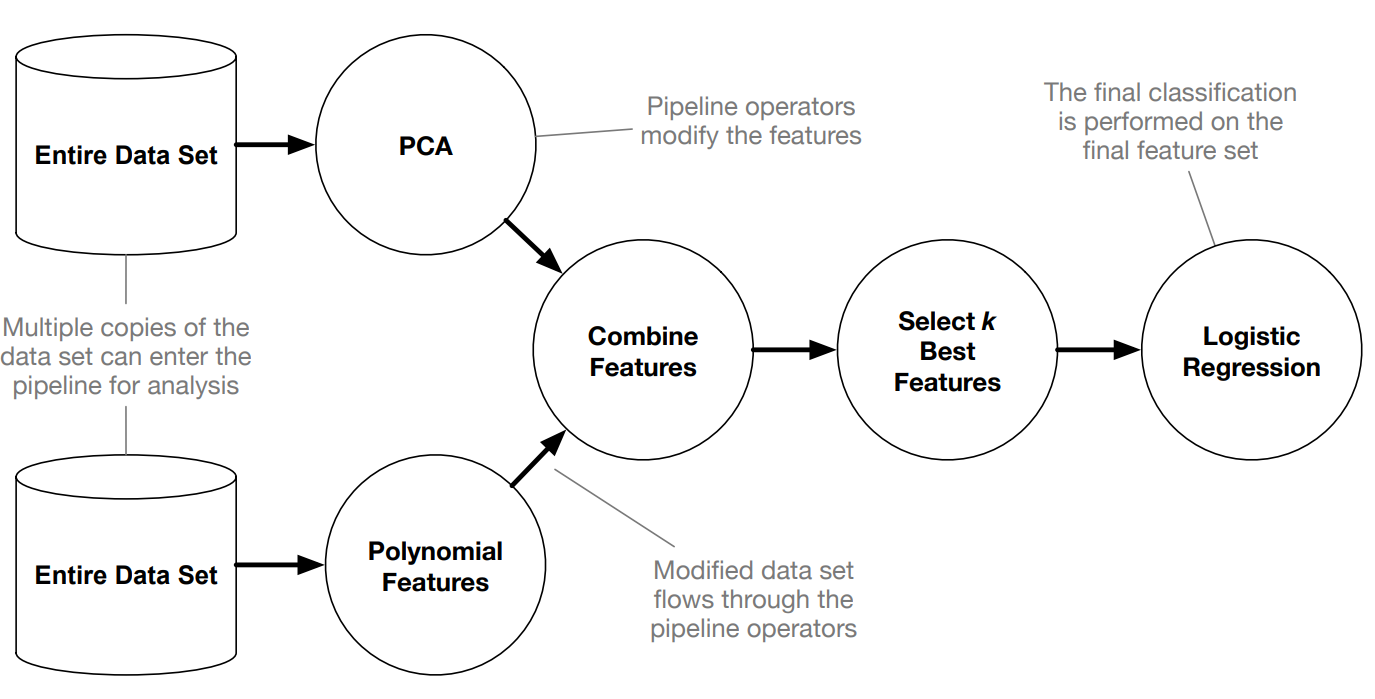
\includegraphics[width=0.8\textwidth]{images/tpot_tree}

\begin{itemize}
  \item TPOT searches in a space of tree-based pipelines
  \item pipeline can potentially grow in size
  \item Challenge: avoid illegal pipelines
\end{itemize}

\end{frame}
%----------------------------------------------------------------------
%----------------------------------------------------------------------
\begin{frame}[c]{Bounds: Distributions instead of Bounds\\ (HyperOpt \litw{Bergstra et al. 2013})}

\begin{itemize}
  \item instead of a range, HyperOpt also allows for user-defined distributions
  \begin{itemize}
    \item sampling of gamma (of SVM) could be done according to\\ log-normal distribution (with given statistics) 
  \end{itemize}
  \item Advantage:\\ allows for flexible definition of expert knowledge
  \item Disadvantage:\\ hard to find a good distribution if expert knowledge is limited
\end{itemize}

\end{frame}
%----------------------------------------------------------------------
%----------------------------------------------------------------------
\begin{frame}[c]{Bounds: Increasing Bounds \litw{Shahriari et al. 2015}}

\begin{enumerate}
  \item start with peaked distributions \\ s.t. it is very unlikely to sample outside of fairly narrow bounds
  \item increase width of distribution over time\\ to search in larger areas over time
\end{enumerate}

\bigskip
\pause

Remark:
\begin{itemize}
  \item similar ideas can be used for safe optimization
  \begin{itemize}
    \item quite important if a failed configuration incurs great (monetary) costs, \\
          a robot is destroyed because of its configuration \lit{Sui et al. 2015}
  \end{itemize}
\end{itemize}

\end{frame}
%----------------------------------------------------------------------
\section{Design Spaces for Neural Networks}
%----------------------------------------------------------------------
\begin{frame}[c]{Design of Neural Networks}

To train a deep neural network, we have many crucial design decisions \hands
\pause

\begin{itemize}
  \item number of layers
  \item number of neurons in each layer
  \item activation functions
  \item skip connections
  \item global architecture (MLP, ResNet, DenseNet, \ldots)
  \item regularization
  \begin{itemize}
    \item batch norm, weight decay, dropout, mixup, cut-out, \ldots 
  \end{itemize}
  \item optimizer hyperparameters
  \begin{itemize}
    \item type of optimizer (SGD, Adam, \ldots)
    \item learning rate
    \item momentum
    \item learning rate schedule
  \end{itemize}
  \item \ldots
\end{itemize}

$\leadsto$ joint global optimization of hyperparameters and architecture!

\end{frame}
%----------------------------------------------------------------------
%----------------------------------------------------------------------
\begin{frame}[c]{Neural Architecture Search (NAS)}

\begin{block}{Neural Architecture Search (NAS)}
Given
\begin{itemize}
  \item a dataset $\dataset$
  \item a design space $\pcs$\\ \textbf{defining the architecture of a deep neural network}
  \item a cost metric or loss function $\loss$ (e.g., predictive error)
\end{itemize}
we want to find the configuration $\conf \in pcs$ minimizing $\loss$ wrt the $\dataset$:

\begin{equation}
\conf^* \in \argmin_{\conf \in \pcs} \loss(\algo(\conf), \dataset) \nonumber
\end{equation}
\end{block}

\end{frame}
%----------------------------------------------------------------------
%----------------------------------------------------------------------
\begin{frame}[c]{Global NAS}

\centering
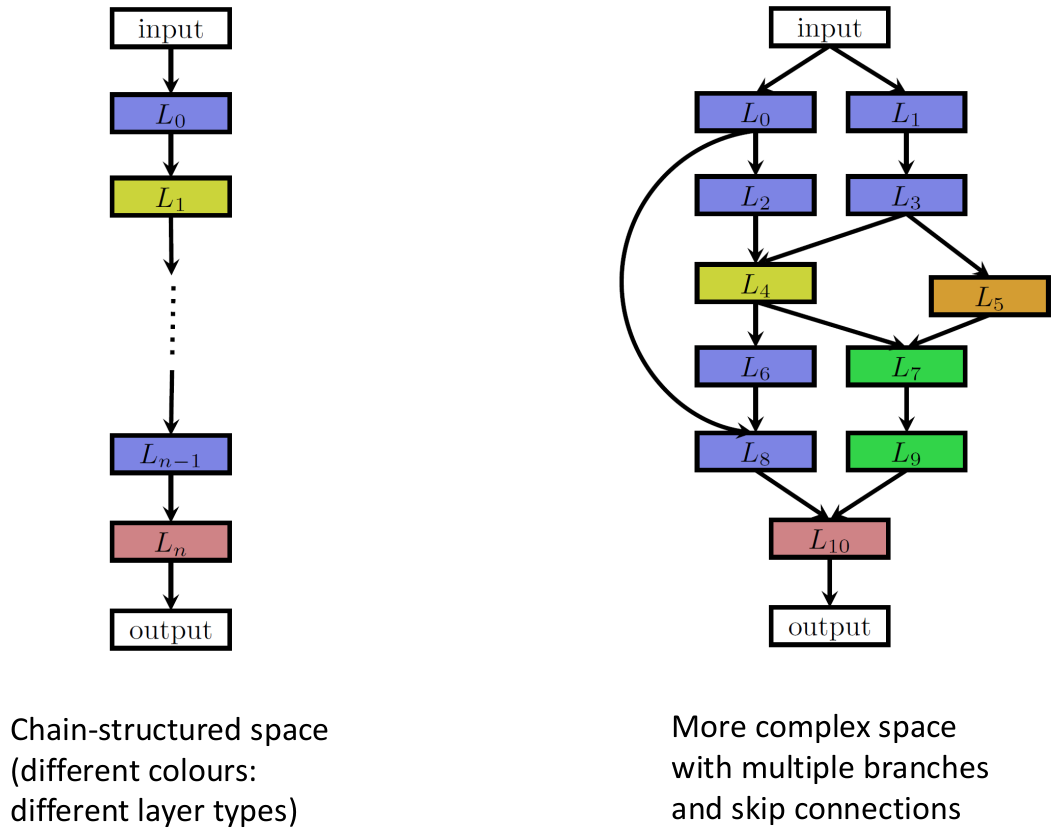
\includegraphics[width=0.7\textwidth]{images/nas_global.png}

\end{frame}
%----------------------------------------------------------------------
%----------------------------------------------------------------------
\begin{frame}[c]{Neural Architecture Search (NAS) -- Remarks}

\begin{itemize}
  \item yet another hyperparameter problem?
  \begin{itemize}
    \item[$\to$] we will see in later sessions how we exploit expert knowledge about neural networks to go beyond black-box HPO
  \end{itemize}
  \pause
  \bigskip
  \item Current practice: 
  \begin{itemize}
    \item hyperparameters (e.g., of the optimizer) are tuned manual or independently from the architecture
  \end{itemize}
  \pause
  \item Better practice:
  \begin{itemize}
    \item jointly optimize hyperparameters and architecture design\\ \lit{Zela et al. 2018}
  \end{itemize}
\end{itemize}

\end{frame}
%----------------------------------------------------------------------
%----------------------------------------------------------------------
\begin{frame}[c]{Shapes of Deep Neural Networks \litw{Kotila 2017}}

\begin{itemize}
  \item Many networks designed by humans follow a pattern
  \item Whether this is a good idea is not well studied
  \item Advantage: The number of hyperparameters is smaller
  \begin{itemize}
    \item E.g., instead of tuning the number of neurons in each layer\\ ($\leadsto$ one hyperparameter per layer),\\
          a few parameters to define shape
  \end{itemize} 
\end{itemize}

\medskip
\centering
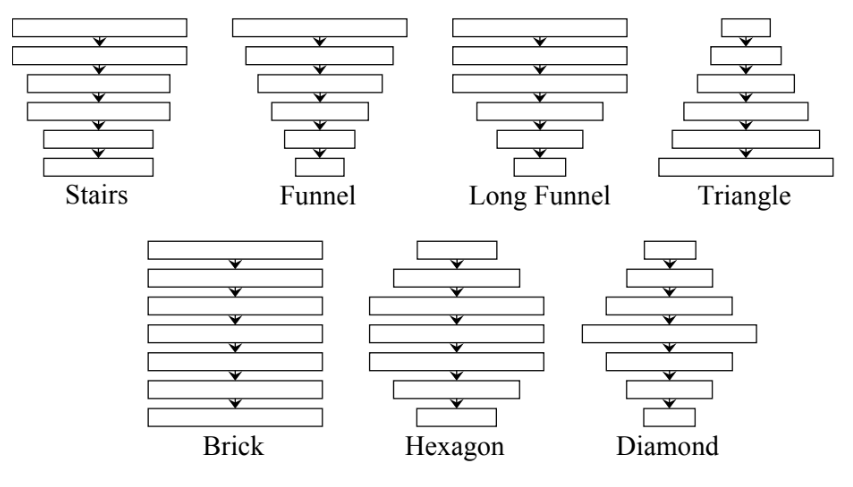
\includegraphics[width=.6\textwidth]{images/nas_shapes.png}

\end{frame}
%----------------------------------------------------------------------
%----------------------------------------------------------------------
\begin{frame}[c]{Cell NAS}

\centering
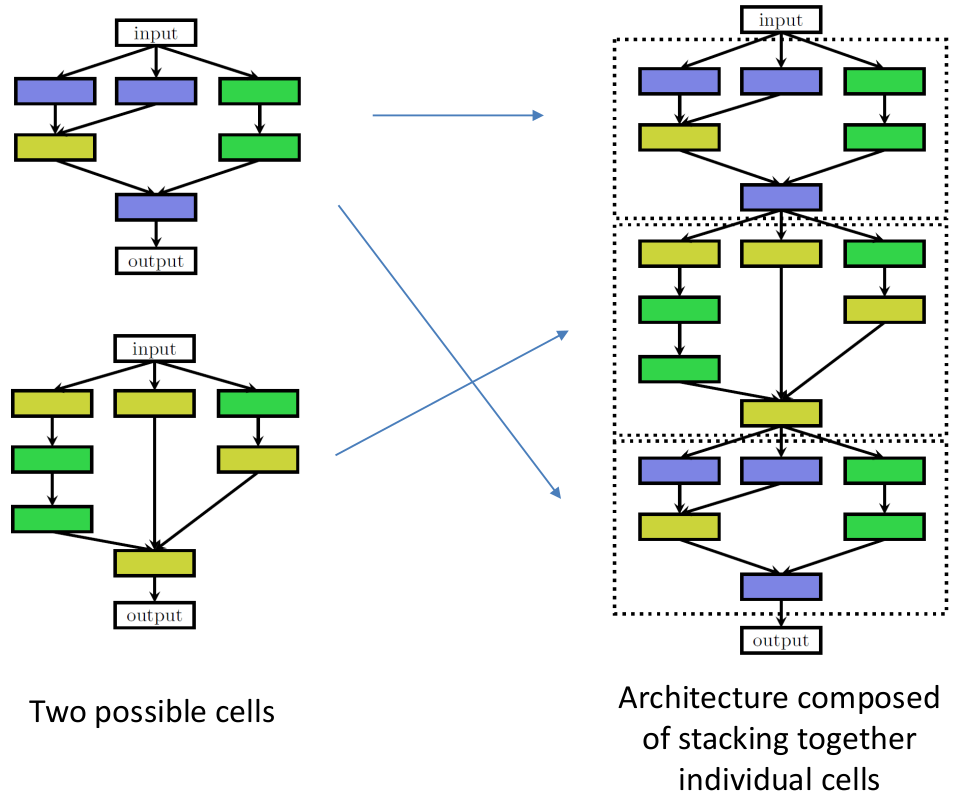
\includegraphics[width=0.7\textwidth]{images/nas_cellsearch.png}

$\leadsto$ Search for cells and repeat these in the final architecture $n$ times.

\end{frame}
%----------------------------------------------------------------------
%----------------------------------------------------------------------
\begin{frame}[c]{Flow of Tensors through Operators}


\begin{columns}
 \column{0.3\textwidth}

\centering
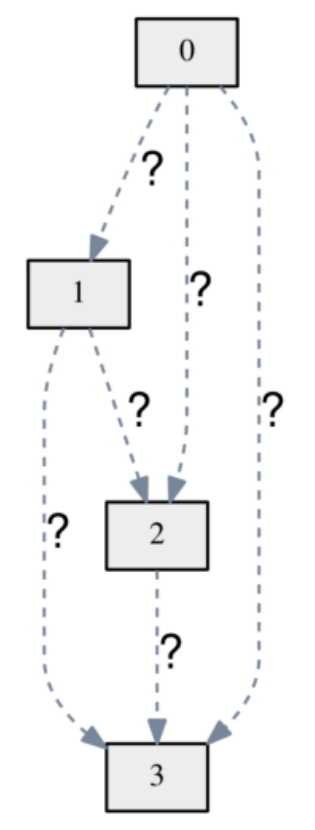
\includegraphics[width=0.6\textwidth]{images/nas_darts_space_idea.png}

 \column{0.7\textwidth}

\begin{itemize}
	\item each node is a tensor (i.e., a latent representation of the input data)
	\item between nodes operators change the data\\ (e.g., convolution or max pooling)
	\begin{itemize}  
		\item includes no-op operators to deactivate edges
	\end{itemize}
\end{itemize}


\begin{flushright}
	Source: \lit{Liu et al. 2019}
\end{flushright}

\end{columns}

\end{frame}
%----------------------------------------------------------------------
%----------------------------------------------------------------------
\begin{frame}[c]{Learning Goals}

Now, you should be able to \ldots

\begin{itemize}
  \item identify design decisions of machine learning algorithms
  \item explain different types of design decisions and there relations
  \item create design spaces
  \item discuss the pro and cons of different design space approaches
  \item explain design spaces for neural architecture search
\end{itemize}

\end{frame}
%----------------------------------------------------------------------
%----------------------------------------------------------------------
\begin{frame}[c]{Literature [These are links]}

\begin{itemize}
	\item \lit{\href{https://www.cs.ubc.ca/~hoos/Publ/Hoos10.pdf}{Programming by Optimization. Hoos 2012}}
	\item \lit{\href{https://ml.informatik.uni-freiburg.de/papers/13-KDD2013-AutoWEKA.pdf}{AutoWEKA and CASH. Thornton et al. 2013}}
	\item \lit{\href{https://www.automl.org/wp-content/uploads/2018/12/tpot.pdf}{TPOT. Olson and Moore. 2019}}
	\item \lit{\href{https://www.automl.org/wp-content/uploads/2018/12/hyperopt-sklearn-1.pdf}{Hyperopt-Sklearn. Komer et al. 2019}}
	\item \lit{\href{http://proceedings.mlr.press/v51/shahriari16.html}{Unbounded Bayesian Optimization via Regularization. Shahriari et al. 2016}}
	\item \lit{\href{https://arxiv.org/abs/1806.09055}{DARTS: Differentiable Architecture Search. Liu et al. 2019}}			
\end{itemize}

\end{frame}
%----------------------------------------------------------------------

%\begin{frame}[c]{}

\centering
\huge
Lecture 3:\\
Evaluation and Visualization
\end{frame}
%----------------------------------------------------------------------
%----------------------------------------------------------------------
\begin{frame}[c]{Where are we? The big picture}

\begin{itemize}
	\item Introduction
	\item[$\to$] Background
	\begin{itemize}
		\item Design spaces in ML
		\item[$\to$] Evaluation and visualization
	\end{itemize}
	\item Hyperparameter optimization (HPO)
	\begin{itemize}
	  \item Bayesian optimization
	  \item Other black-box techniques
	  \item Speeding up HPO with multi-fidelity optimization
	\end{itemize}
	\item Pentecost (Holiday) -- no lecture
	\item Architecture search I + II
	\item Meta-Learning
	\item Learning to learn $\&$ optimize
	\item Beyond AutoML: algorithm configuration and control
	\item Project announcement and closing
\end{itemize}


\end{frame}
%----------------------------------------------------------------------
%----------------------------------------------------------------------
\begin{frame}[c]{Learning Goals}

After this lecture, you will be able to \ldots

\begin{itemize}
	\item explain the role of outliers in CS/ML
	\item compare and visualize the performance of different configurations
	\item compare and visualize the performance of AutoML systems
	\item explain and correctly apply statistical hypothesis tests
\end{itemize}

\end{frame}
%----------------------------------------------------------------------

%----------------------------------------------------------------------
\begin{frame}[c]{How CS differs from other empirical sciences}

\begin{itemize}
	\item We have a complete and precise \alert{mathematical description}\\of the object under study
	\smallskip
	
	\item We have complete and precise \alert{control} of the object under study\\ 
	(and to some degree also the experimental environment)
	\begin{itemize}
		\item as a result, experiments can be \alert{reproduced perfectly}
		\pause
		\item what do we need for experiments to be reproducible? 
		\only<2-2>{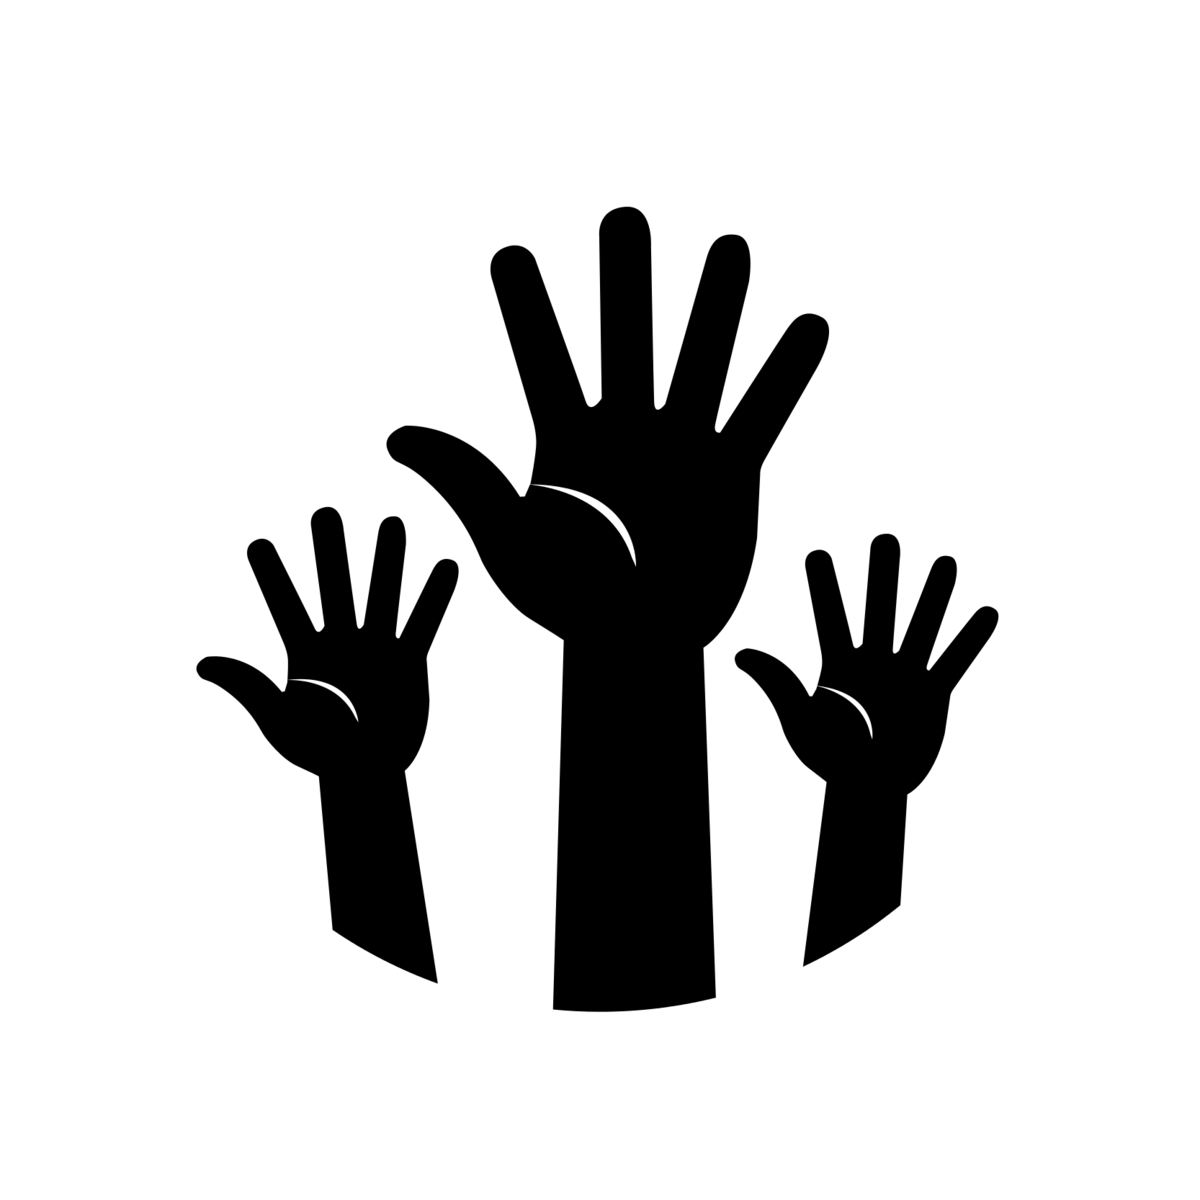
\includegraphics[height=1.5em]{images/hands}
		}
		\only<3->{
			\begin{itemize}
				\item  {Code \& dependencies, inputs, environment ($\rightarrow$ VM \& cloud)}
			\end{itemize}
			\pause
		}
	\end{itemize}
	\medskip
	\pause
	
	%\only<4->{
	\item We often have quite \alert{cheap} experiments
	\begin{itemize}
		\item price for computers is monotonically decreasing
		\item often maximal runtimes of 1h; exception: deep learning (up to a week)
		\item compare e.g., experimental physics: 1 week of beam time per year % Still different from observing new species in the field for half a year / 
	\end{itemize}
	\smallskip
	\pause
	%}
	%\only<5->{
	\item We can conduct and analyze experiments fully \alert{automatically} 
	\begin{itemize}
		\item we can gather large amounts of data quickly (e.g., 100 repetitions)
		\item but: don't confuse statistical significance and relevance
	\end{itemize}
	%}	
\end{itemize}

\end{frame}
%-----------------------------------------------------------------------
%----------------------------------------------------------------------
\begin{frame}[c]{Outliers are quite different in computer experiments}

Is the following statement correct? 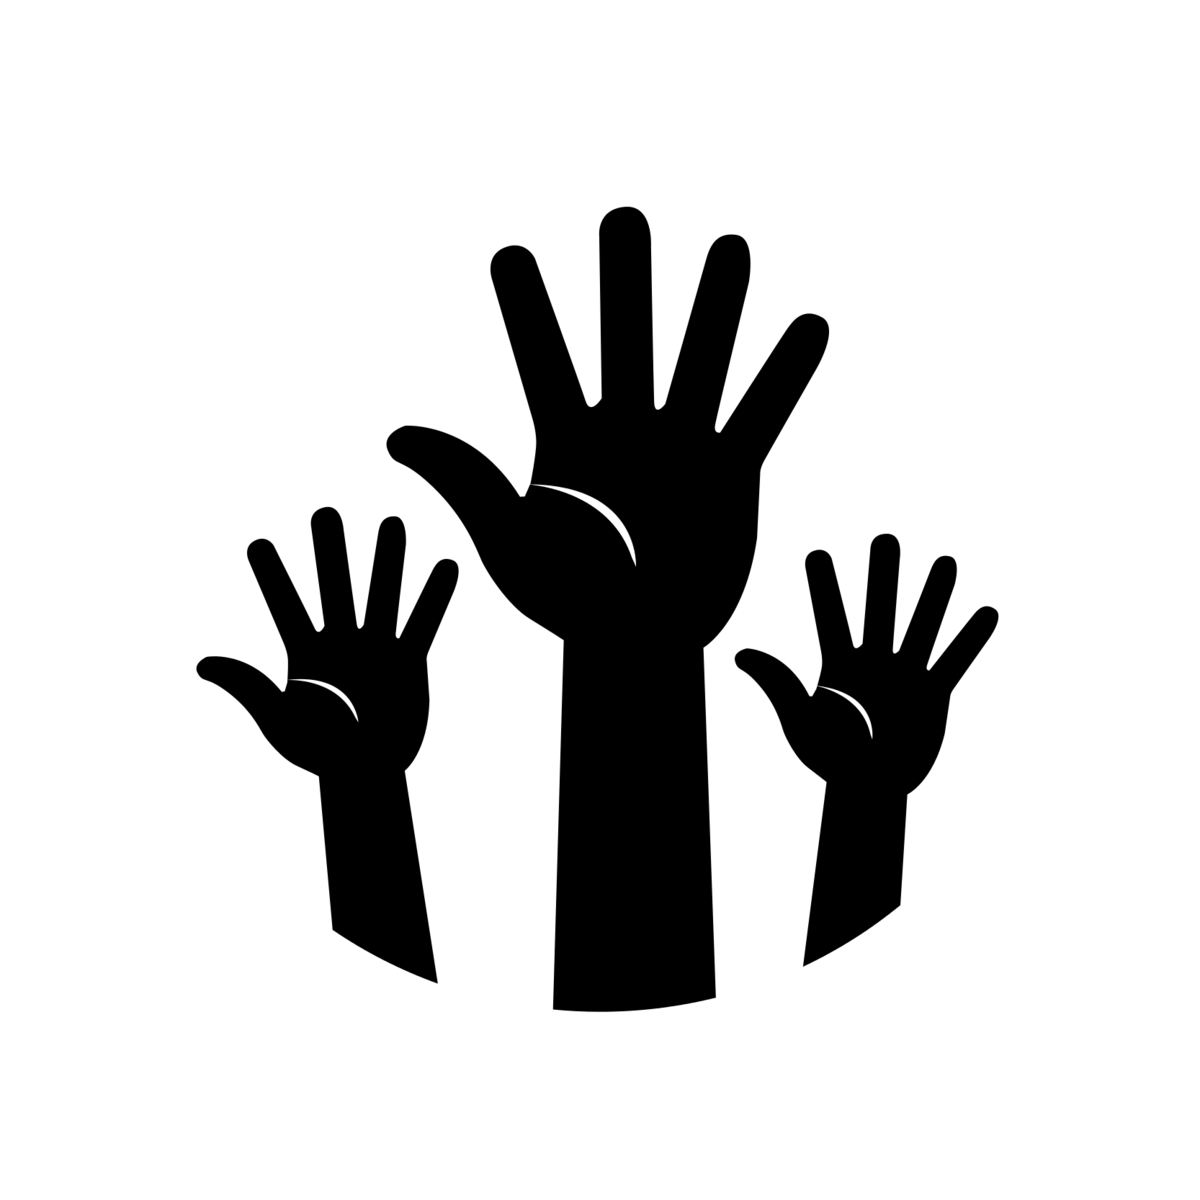
\includegraphics[height=1.5em]{images/hands}

``As usual in other empirical sciences, we (in CS) should take care to \alert{detect and remove outliers} before further analysis.''

\pause
\bigskip

\begin{block}{Outliers in CS/ML}
\begin{itemize}
	\item outliers should be investigated closely -- why is there an outlier?
	\item outliers are (hopefully) reproducible -- narrow down their reason!
	\pause
	\begin{itemize}
		\item \textbf{Algorithm:} When characterizing performance of an optimization algorithm, \alert{outliers with poor values can indicate (deep) local optima}
		\pause
		\item \textbf{Environment:} Outliers can indicate a \alert{problem with the environment} (e.g., file system or network issues)
		\pause
		\item \textbf{Datasets:}  When characterizing cost across a distribution of datasets, outliers with small values can indicate trivial datasets.
	\end{itemize}
\end{itemize}
\end{block}

\end{frame}
%-----------------------------------------------------------------------
\section{Visualization of Configuration Performance}
%----------------------------------------------------------------------
%----------------------------------------------------------------------
\begin{frame}[c]{Setup}

For the following slides, we have used the following setup:

\begin{itemize}
	\item Model: simple MLP (from sklearn)\\ with 2 layers with 128 neurons and 64 neurons, resp.
	\item Dataset: Digits  
	\item Setting 1: learning rate of $0.001$ 
	\item Setting 2: learning rate of $0.01$
\end{itemize}


\end{frame}
%----------------------------------------------------------------------

%----------------------------------------------------------------------
\begin{frame}[c]{A Single Learning Curve (Setting 1)}

\centering
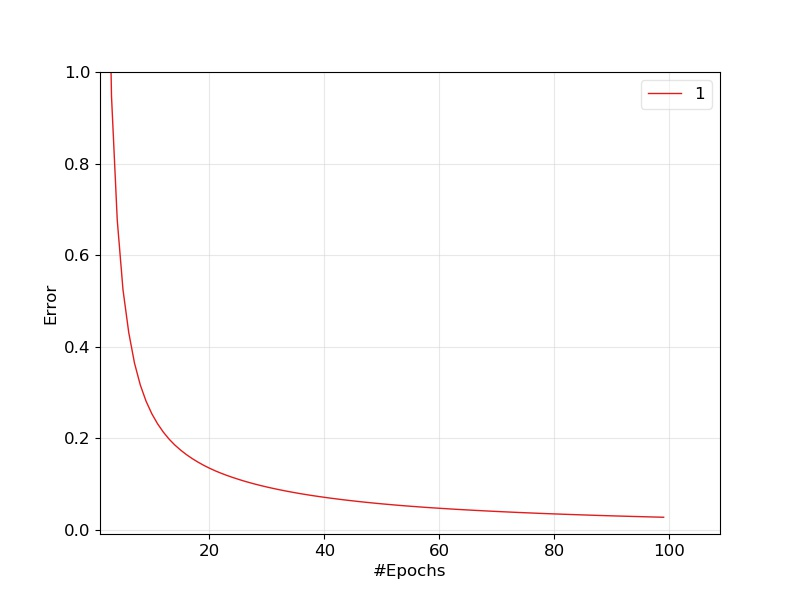
\includegraphics[width=0.8\textwidth]{scripts/one_learning_curve.jpg}


\end{frame}
%----------------------------------------------------------------------
%----------------------------------------------------------------------
\begin{frame}[c]{$10$ Learning Curves  (Setting 1)}

\centering
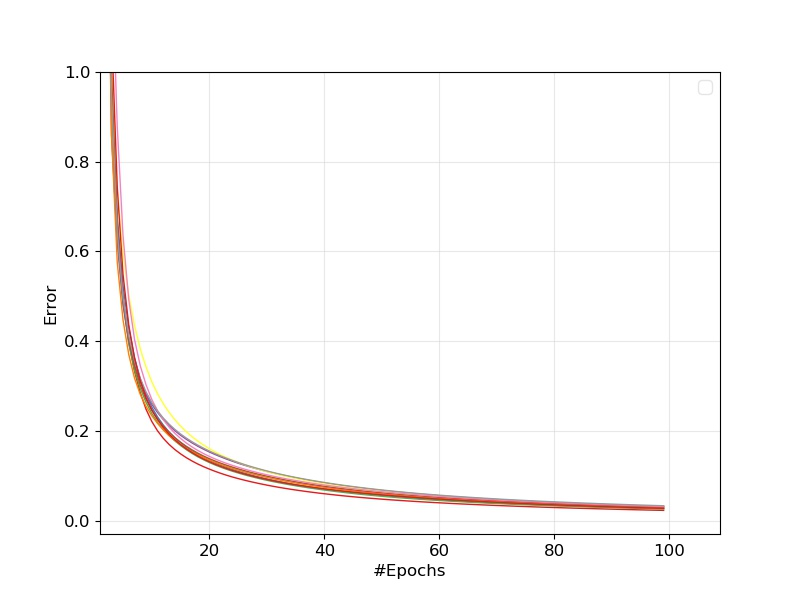
\includegraphics[width=0.6\textwidth]{scripts/ten_learning_curves.jpg}

\begin{itemize}
	\item[$\leadsto$] Deep learning (and most other ML algorithms) are non-deterministc
	\item[$\leadsto$] Measure performance more than once and estimate noise-level
\end{itemize}


\end{frame}
%----------------------------------------------------------------------
%----------------------------------------------------------------------
\begin{frame}[c]{Aggregated Learning Curves (Setting 1)}

\centering
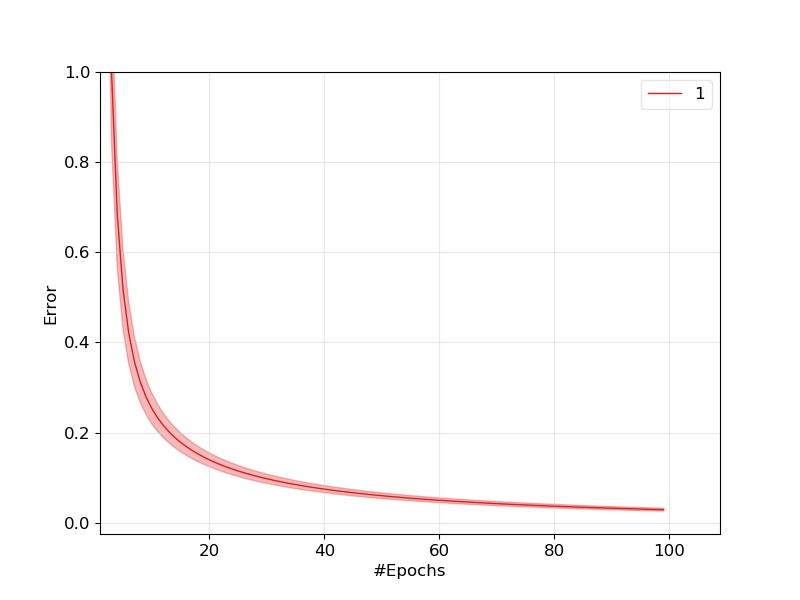
\includegraphics[width=0.6\textwidth]{scripts/hundred_agg_learning_curves.jpg}

\begin{itemize}
	\item Plot mean and stdev (shaded area) across $n$ (here $100$) random seeds\\
	\item Only use mean and stdev
	if noise is somehow normal distributed
	\item alternatives are the mean+standard error or median+25/75-percentiles
\end{itemize}

\end{frame}
%----------------------------------------------------------------------
%----------------------------------------------------------------------
\begin{frame}[c]{Comparing Learning Curves}

\centering
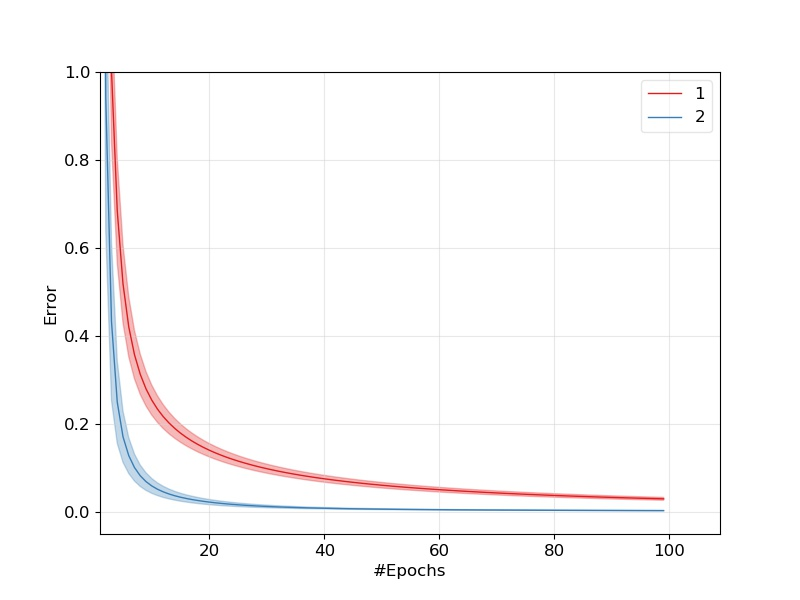
\includegraphics[width=0.7\textwidth]{scripts/compare_learning_curves.jpg}

\begin{itemize}
	\item If uncertainties (shaded area) overlap, results might not be statistically significant but due to noise
\end{itemize}

\end{frame}
%----------------------------------------------------------------------
%----------------------------------------------------------------------
\begin{frame}[c]{Scatter Plot: Train vs. Test}


\begin{columns}
	
\column{0.5\textwidth}

\centering
Setting 1
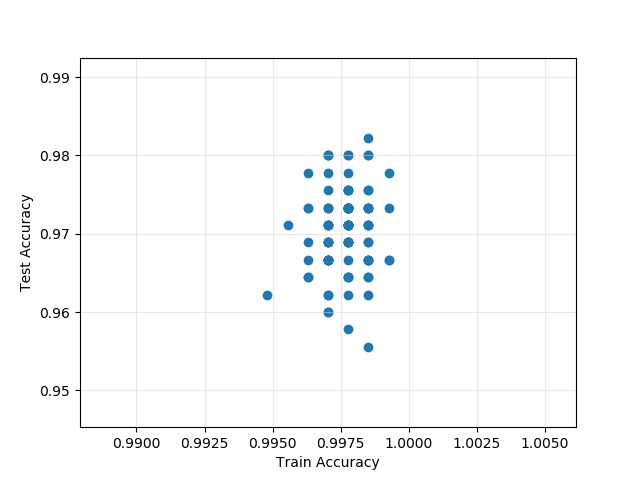
\includegraphics[width=1\textwidth]{scripts/mlp1_test_train_scatter.jpg}

\begin{itemize}
	\item perfect would be if train and test score are correlated
	\item here at least not anti-correlated
\end{itemize}


\column{0.5\textwidth}

\pause
\centering
Setting 2
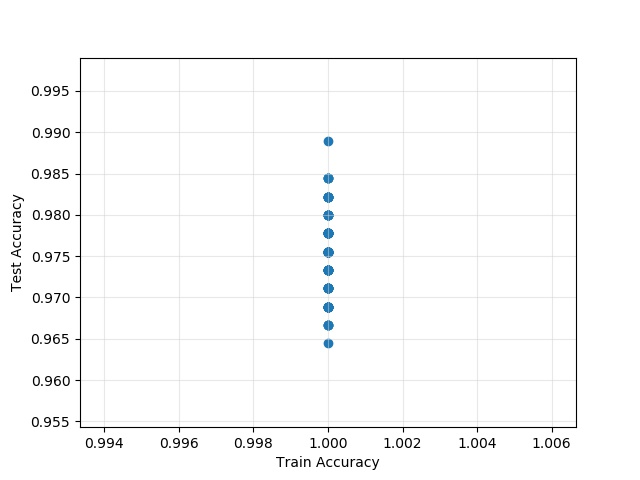
\includegraphics[width=1\textwidth]{scripts/mlp2_test_train_scatter.jpg}
	
\begin{itemize}
	\item already perfect training score
	\item generalization nevertheless noisy
\end{itemize}
	
\end{columns}
	
\end{frame}
%----------------------------------------------------------------------
%----------------------------------------------------------------------
\begin{frame}[c]{eCDF: Distribution of Performance (Setting 1)}

\centering
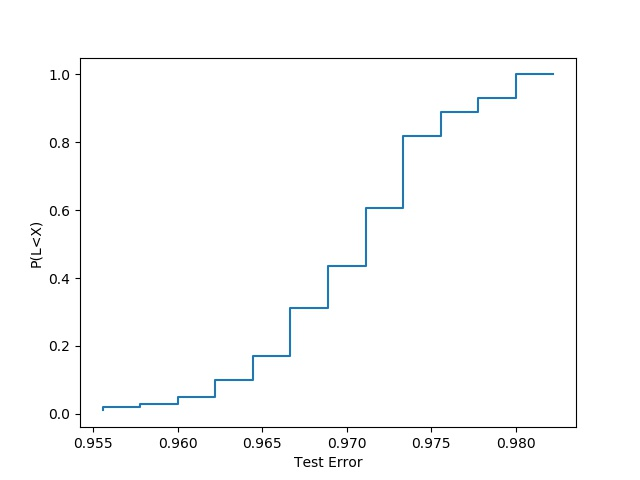
\includegraphics[width=0.6\textwidth]{scripts/mlp1_test_ecdf.jpg}

\begin{flushleft}
	How to compute an empirical CDF:
	\begin{enumerate}
		\item X: sorted error scores
		\item Y: $[1\ldots\#\text{points}] / \#\text{points}$
		\item step\_function(X,Y)
	\end{enumerate}
\end{flushleft}


\end{frame}
%----------------------------------------------------------------------
%----------------------------------------------------------------------
\begin{frame}[c]{eCDF: Distribution of Performance}

\centering
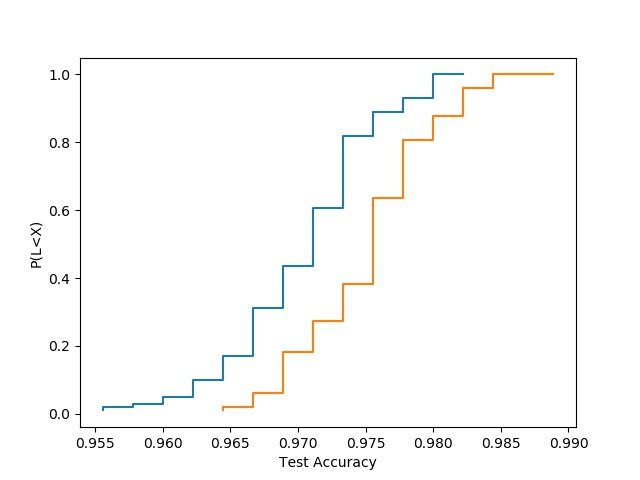
\includegraphics[width=0.6\textwidth]{scripts/mlp12_test_ecdf.jpg}


Which curve corresponds to which setting? \hands

\end{frame}
%----------------------------------------------------------------------
%----------------------------------------------------------------------
\begin{frame}[c]{Box Plot: Comparing Two Configurations}

\centering
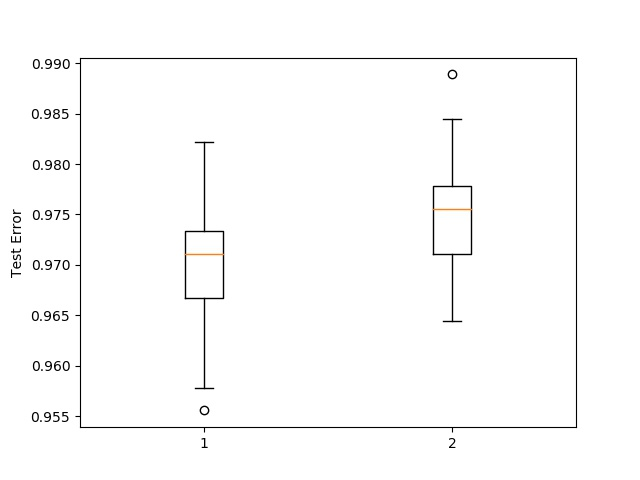
\includegraphics[width=0.6\textwidth]{scripts/mlp12_boxplot.jpg}

\begin{itemize}
	\item alternative: violin plots
	\pause
	\smallskip
	\item if you have paired populations (e.g., configurations evaluated on different datasets),
			you should generate boxplots with $\loss / \loss_{\text{baseline}}$ 
	\item[$\leadsto$] insight on how many datasets one of the two performed better
\end{itemize}
	

\end{frame}
%----------------------------------------------------------------------
%-----------------------------------------------------------------------
\section{Visualization of AutoML Performance}
%----------------------------------------------------------------------
%----------------------------------------------------------------------
\begin{frame}[c]{AutoML Systems over Time}

\begin{itemize}
	\item Don't only measure the performance of AutoML systems for a fixed budget because:
	\begin{enumerate}
	   \item A priori, it is unknown how long a user will run an AutoML system
	   \item Some systems perform well for small budgets and some others need more time before performing well
	   \begin{itemize}
	   	\item BO-based systems often perform as good as\\ random search in the beginning, but perform very well later on
	   \end{itemize}
    \end{enumerate}
	\pause
	\item[$\leadsto$] AutoML systems should have a good anytime performance
	\pause
	\medskip
	\item Recommendation: plot performance (e.g., error) over time
	\begin{itemize}
		\item Similar to learning curves of DNNs 
	\end{itemize} 
\end{itemize}


\end{frame}
%----------------------------------------------------------------------
%----------------------------------------------------------------------
\begin{frame}[c]{Aggregated AutoML Systems over Time}

\centering
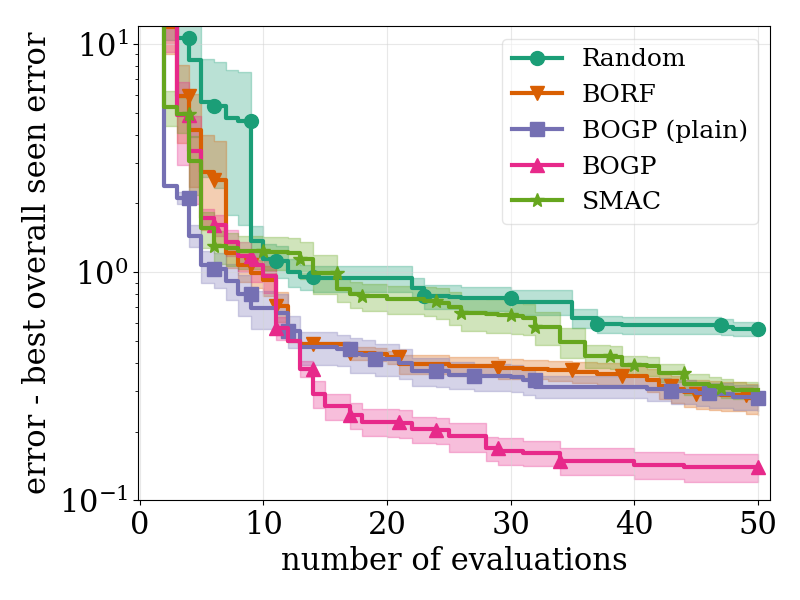
\includegraphics[width=0.5\textwidth]{images/MLPOnMnist_tFalse.png}

\begin{itemize}
	\item Different HPO systems minimizing the error of an MLP on MNIST
	\item How to do it:
	\begin{itemize}
		\item Run each systems several times and always log its current incumbent 
		\item Plot mean and stdev for each system after each incumbent update
		\item Use step functions, because linear interpolation would be\\ too optimistic
	\end{itemize}
\end{itemize}

\end{frame}
%----------------------------------------------------------------------
%----------------------------------------------------------------------
\begin{frame}[c]{Aggregated AutoML Systems over Time and Datasets}

\begin{itemize}
	\item An AutoML system should not only perform well on a single dataset but on many datasets
	\item To summarize and compare the performance across a set of datasets,
	we can plot the performance over time and across datasets
	\pause
	\item Ways to do it:
	\begin{enumerate}
		\item Average loss metric (e.g., error) across datasets
		\begin{itemize}
			\item Problem: different scales of errors on different datasets
		\end{itemize}
	    \pause
	    \item Normalize loss metric across datasets,\\
	    e.g., best seen loss relates to a zero cost
	    \begin{itemize}
	    	\item Problem: Minor improvements ($\leq 0.1\%$) might look substantial
	    \end{itemize}
	\end{enumerate}
    \pause
    \item[$\leadsto$] There is no way around that you have some kind of information loss 
\end{itemize}

\end{frame}
%----------------------------------------------------------------------
%----------------------------------------------------------------------
\begin{frame}[c]{Ranked AutoML Systems over Time and Datasets}


\centering
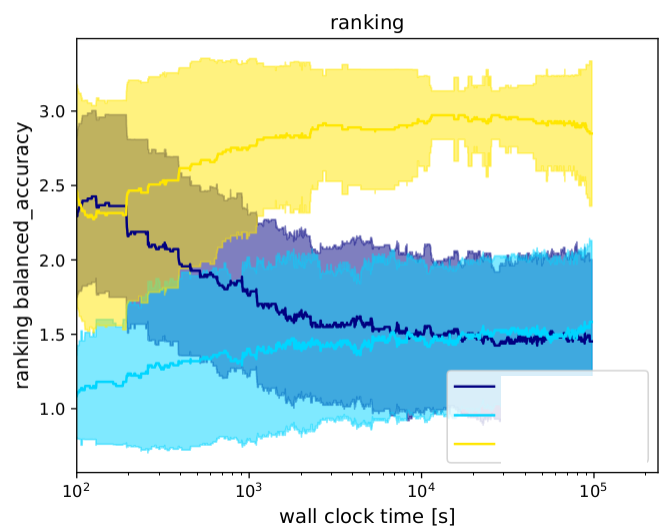
\includegraphics[width=0.5\textwidth]{images/rankings_over_time.png}

\begin{itemize}
	\item Remarks:
	\begin{itemize}
		\item x-axis should be on log-scale
		\item uncertainties (shaded areas) can be obtained via bootstrap sampling
	\end{itemize}
    \pause
    \smallskip
	\item Ranks avoid the problem of different scales
	\item Problem: we don't know whether a better ranking relates to a substantial improvement of the actual cost metric
\end{itemize}

\end{frame}
%----------------------------------------------------------------------
%----------------------------------------------------------------------
\begin{frame}[c]{Scatter Plot: Meta Features}

\begin{columns}
	\column{0.5\textwidth}
	
	\centering
	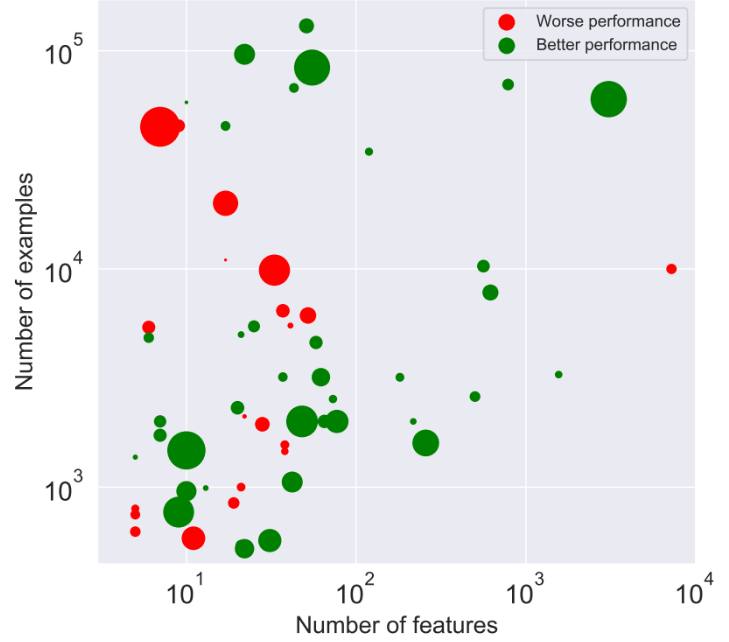
\includegraphics[width=1.0\textwidth]{images/scatter_dataset_twoconfigs.png}
	
	\column{0.5\textwidth}
	\begin{itemize}
		\item Compare two systems\\ (or 1 vs rest)
		\item each dot is a dataset
		\item color encoding better or worse
		\item size indicates performance difference
		\item meta-features (e.g., \#features, \#samples) on axes
		\begin{itemize}
			\item using PCA on a larger set of meta-features leads to algorithm footprints \lit{Smith-Miles et al. 2012}
		\end{itemize}
	\end{itemize}
\end{columns}


\end{frame}
%----------------------------------------------------------------------
%----------------------------------------------------------------------
\begin{frame}[c]{Heatmaps: Comparing several Configurations}

\begin{columns}
	\column{0.5\textwidth}
	
	\centering
	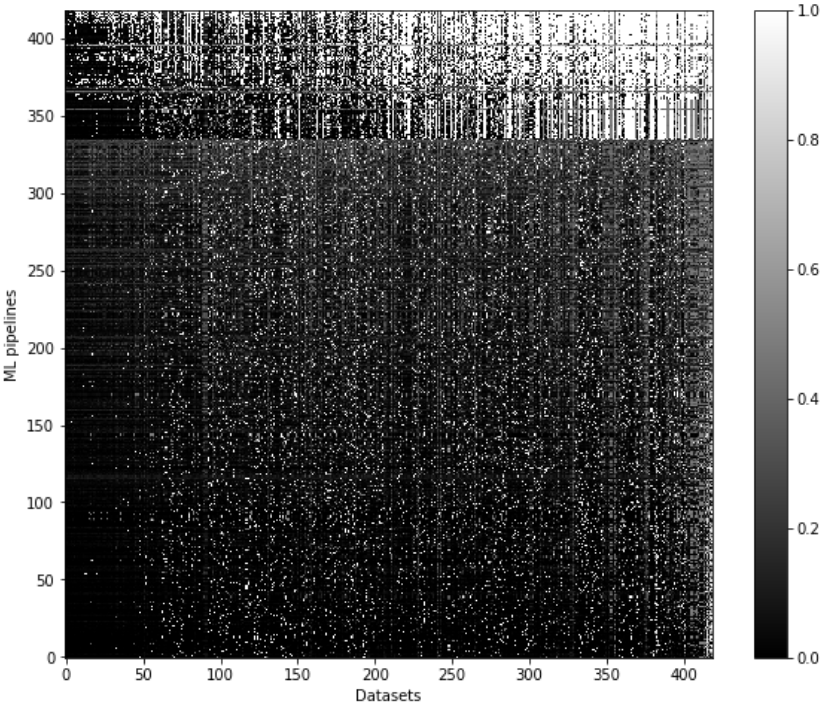
\includegraphics[width=1.0\textwidth]{images/heatmap_pipelines.png}
	
	\column{0.5\textwidth}
	
	\begin{itemize}
		\item compare many configurations on many datasets
		\item can reveal:
		\begin{itemize}
			\item homogeneity if smooth transition from hard to easy
			\item heterogeneity if stripes exist (here the case) 
		\end{itemize}
	    \item Remark: datasets and configurations should be sorted according to their average cost
	\end{itemize}
	
\end{columns}

\end{frame}
%----------------------------------------------------------------------
%-----------------------------------------------------------------------
\section{Statistical Hypothesis Testing}
%----------------------------------------------------------------------
\begin{frame}[c]{Background: statistical hypothesis tests}

\begin{itemize}
	\item When we have a lot of data, we need to summarize it
	\begin{itemize}
		\item But we already saw that summarization hides a lot of data
		%	  \item E.g., a single outlier might explain the difference in means
		\item Ideally, we want to draw high-level conclusions\\
		(e.g., ``A outperforms B on datasets of type X'')
	\end{itemize}
	
	\pause
	\bigskip
	
	\item Problem: we only have a finite number of observations
	\begin{itemize}
		\item Can we attribute observed performance differences to chance?
		\item Are we reasonably sure that a claim we make is reproducible?
		\item[$\leadsto$] Statistical tests can help
	\end{itemize}
	
	
\end{itemize}

\medskip

\end{frame}
%-----------------------------------------------------------------------
%----------------------------------------------------------------------
\begin{frame}[c]{Statistical hypothesis testing}

\begin{enumerate}
\item Define initial research hypothesis
\pause
\item Derive null $H_0$ and alternative $H_1$ hypothesis
\begin{itemize}
	\item Alternative hypothesis should be your research hypothesis
\end{itemize}
\end{enumerate}	

\end{frame}
%-----------------------------------------------------------------------
%----------------------------------------------------------------------
\begin{frame}[c]{First example: Courtroom Tiral}

\begin{itemize}
\item A prosecutor tries to prove the guilt of the defendant
\item $H_0$: 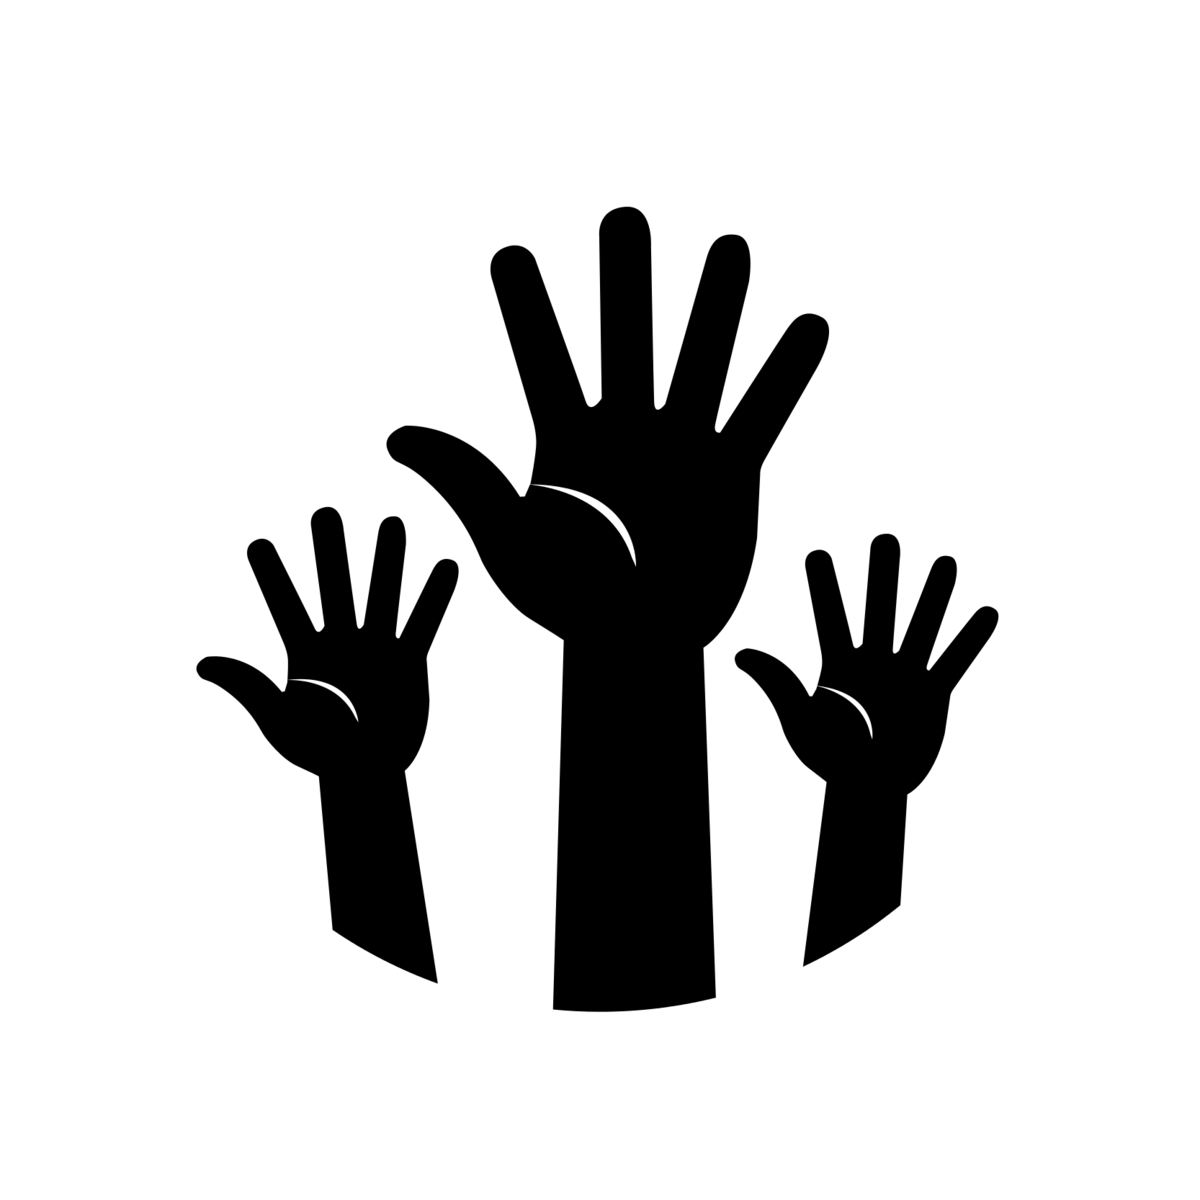
\includegraphics[height=1em]{images/hands} \only<2->{The defendant is not guilty
\begin{itemize}
	\item Accepted for the moment\\ (``not guilty as long as their guilt is not proven'') 
\end{itemize}
}
\item $H_1$: 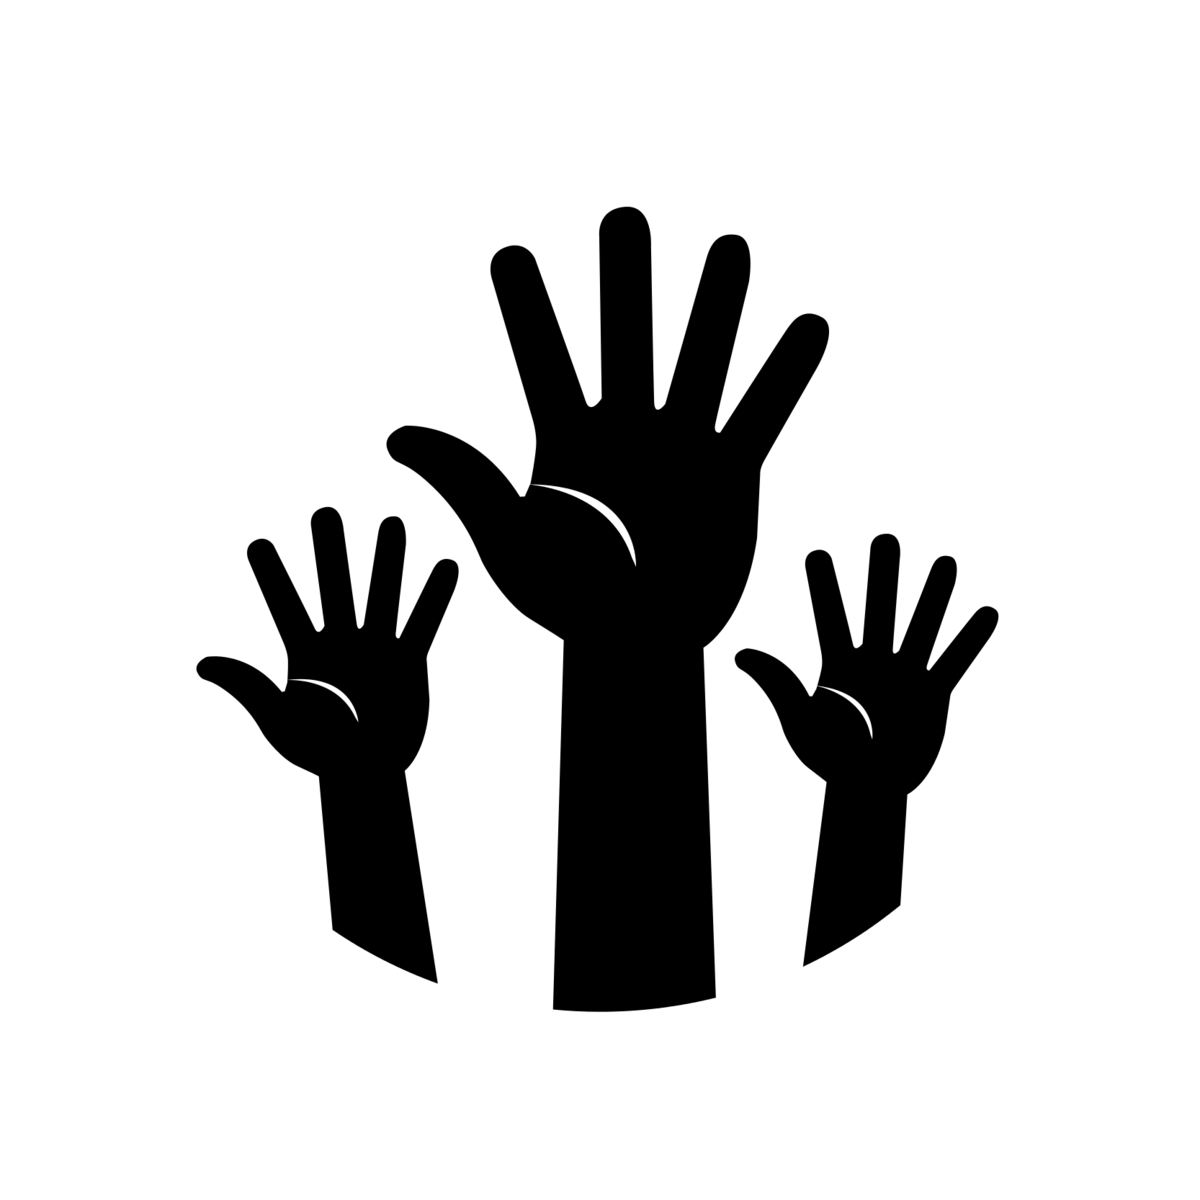
\includegraphics[height=1em]{images/hands} \only<2->{The defendant is guilty
\begin{itemize}
	\item prosecutor hopes to support that
\end{itemize}
}
\pause
\end{itemize}

\medskip
\pause
\bigskip
\centering
\begin{tabular}{c|cc}
\toprule
& Truly not guilty 	& Truly guilty\\
\hline
Acquittal 	& Right decision	& Type II Error\\
Conviction & Type I Error		& Right decision\\
\bottomrule
\end{tabular}	

\bigskip
$\leadsto$ We want to minimize Type I error!

\end{frame}
%-----------------------------------------------------------------------
%----------------------------------------------------------------------
\begin{frame}[c]{Statistical hypothesis testing (cont'd)}

\begin{enumerate}
\item Define initial research hypothesis
\item Derive null $H_0$ and alternative $H_1$ hypothesis
\begin{itemize}
\item Alternative hypothesis should be your research hypothesis
\end{itemize}
\item Consider statistical assumptions
\begin{itemize}
\item E.g., is your data Gaussian distributed?
\end{itemize}
\pause
\item Decide test and test statistic $T$
\begin{itemize}
\item The correct test depends on your statistical assumptions.
\item Typically: if you use more assumptions, the test is more powerful\\ (i.e., less Type-I error)
\end{itemize}
\pause
\item Decide significance level $\alpha$\\ (i.e., acceptable Type-I error to reject null hypothesis)
\pause
\item Compute observed $t_{obs}$ of test statistic $T$
\item Calculate $p$-value given $t_{obs}$
\begin{itemize}
\item i.e., probability under the null hypothesis of sampling a test statistic as extreme as observed (probability of Type-I error)
\end{itemize} 
\pause
\item If $p < \alpha$, reject null hypothesis in favor of alternative hypothesis
\begin{itemize}
\item If $p > \alpha$, it doesn't tell you anything about the null hypothesis!
\end{itemize}
\end{enumerate}	

\end{frame}
%-----------------------------------------------------------------------
%----------------------------------------------------------------------
\begin{frame}[c]{Second example for a statistical test}

\begin{itemize}
\item IQ values are known to be normally distributed with $X \sim
\mathcal{N}(100,15)$
\begin{itemize}
\item$\to$ statistical assumption
\end{itemize}
% \\with mean $100$ and variance $15$: $X \sim \mathcal{N}(100,15)$
\item Claim: \alert{``the students in this class are more intelligent
than average''}
\bigskip
\pause
\item \alert{Null Hypothesis $H_0$}: $\mu=100$ ($\mu$ is the population
mean of this class)
\item \alert{Alternative Hypothesis $H_1$}: $\mu>100$ (\alert{one-sided} hypothesis)

\bigskip
\pause

\item Let's say we observed IQ values $x_i$ of 9 students in the class:
\begin{itemize}
\item $\{x_1,\dots,x_9\} = \{116, 128, 125, 119, 89, 99, 105, 116, 118\}$.
\item The \alert{sample mean} is $\bar{x}=112.8$
\item Does this data support the claim?
\end{itemize}	

\end{itemize}	

\end{frame}
%-----------------------------------------------------------------------
%----------------------------------------------------------------------
\begin{frame}[c]{Example continued}

\begin{itemize}

\item \alert{Distribution of the test statistic} 
\begin{itemize}
\item Under $H_0$, we know that each $x_i \sim \mathcal{N}(100,15)$
\smallskip
\item The \alert{test statistic} that we measure is the sample
mean $\bar{x} = \frac{1}{9} \sum_{i=1}^9 x_i$
%    \item[-] $\bar{x} \sim  \mathcal{N}(\mu=100,\sigma^2=15/\sqrt{n})=\mathcal{N}(100,5)$
\bigskip
\pause
\item Under $H_0$, the distribution of $\bar{x}$ is
$\mathcal{N}(100,15/\sqrt{9})$
\begin{itemize}
\item[-] Our observation $\bar{x}=112.8$ is quite extreme under that
distribution
\end{itemize}
\end{itemize}	
\end{itemize}

\begin{center}
%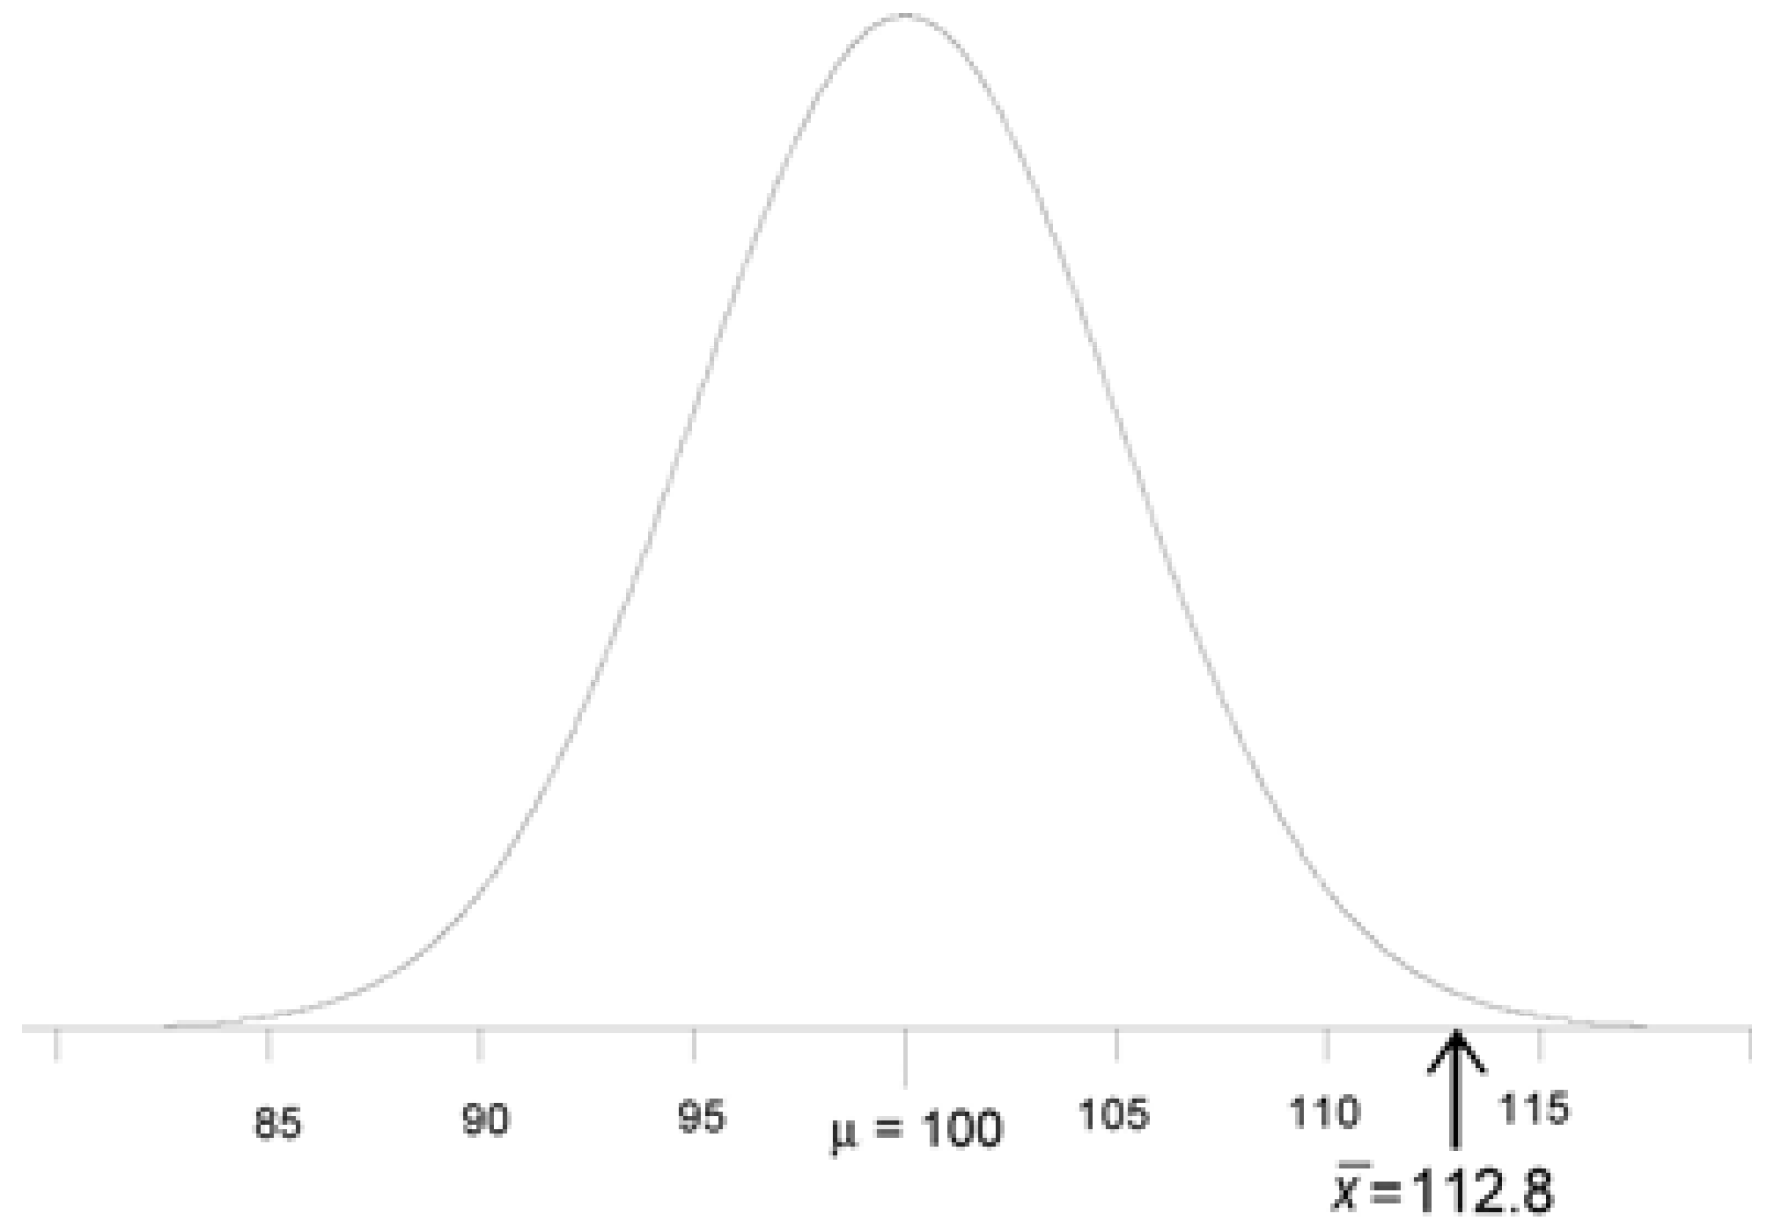
\includegraphics[height=3cm]{images/z_test_1.png}


\pgfmathdeclarefunction{gauss}{2}{%
	\pgfmathparse{1/(#2*sqrt(2*pi))*exp(-((x-#1)^2)/(2*#2^2))}%
}
\tikzstyle{myarrow}=[->, thick]
\begin{tikzpicture}
\begin{axis}[scale=0.75,
no markers, domain=82:118, samples=100,
axis lines*=left, xlabel=$IQ$,axis y line=none,
every axis x label/.style={at=(current axis.right of origin),anchor=west},
every x tick label/.append style={font=\scriptsize, yshift=0.5ex},
height=5cm, width=12cm,label style={font=\tiny},
xtick={80, 85, 90, 95, 100, 105, 110, 115, 120},
xticklabels={$80$, $85$, $90$, $95$, $100$, $105$, $110$, $115$, $120$},
ytick=\empty,
enlargelimits=false, clip=false, axis on top,
x=0.25cm, y=0.25cm/.004,
]
\addplot [thick,cyan!50!black] {gauss(100,15/sqrt(9))};
\coordinate (stat) at (axis cs:112.8,0.00325);
\coordinate (statlabel) at (axis cs:112.8,-.01);
\draw[myarrow, black!75] (statlabel) node [below, font=\scriptsize] {$\bar{x}=112.8$} -- (stat);
\end{axis}

\end{tikzpicture}
\end{center}

\end{frame}
%-----------------------------------------------------------------------
%----------------------------------------------------------------------
\begin{frame}[c]{General principle}

\vspace*{-0.2cm}
\begin{center}
%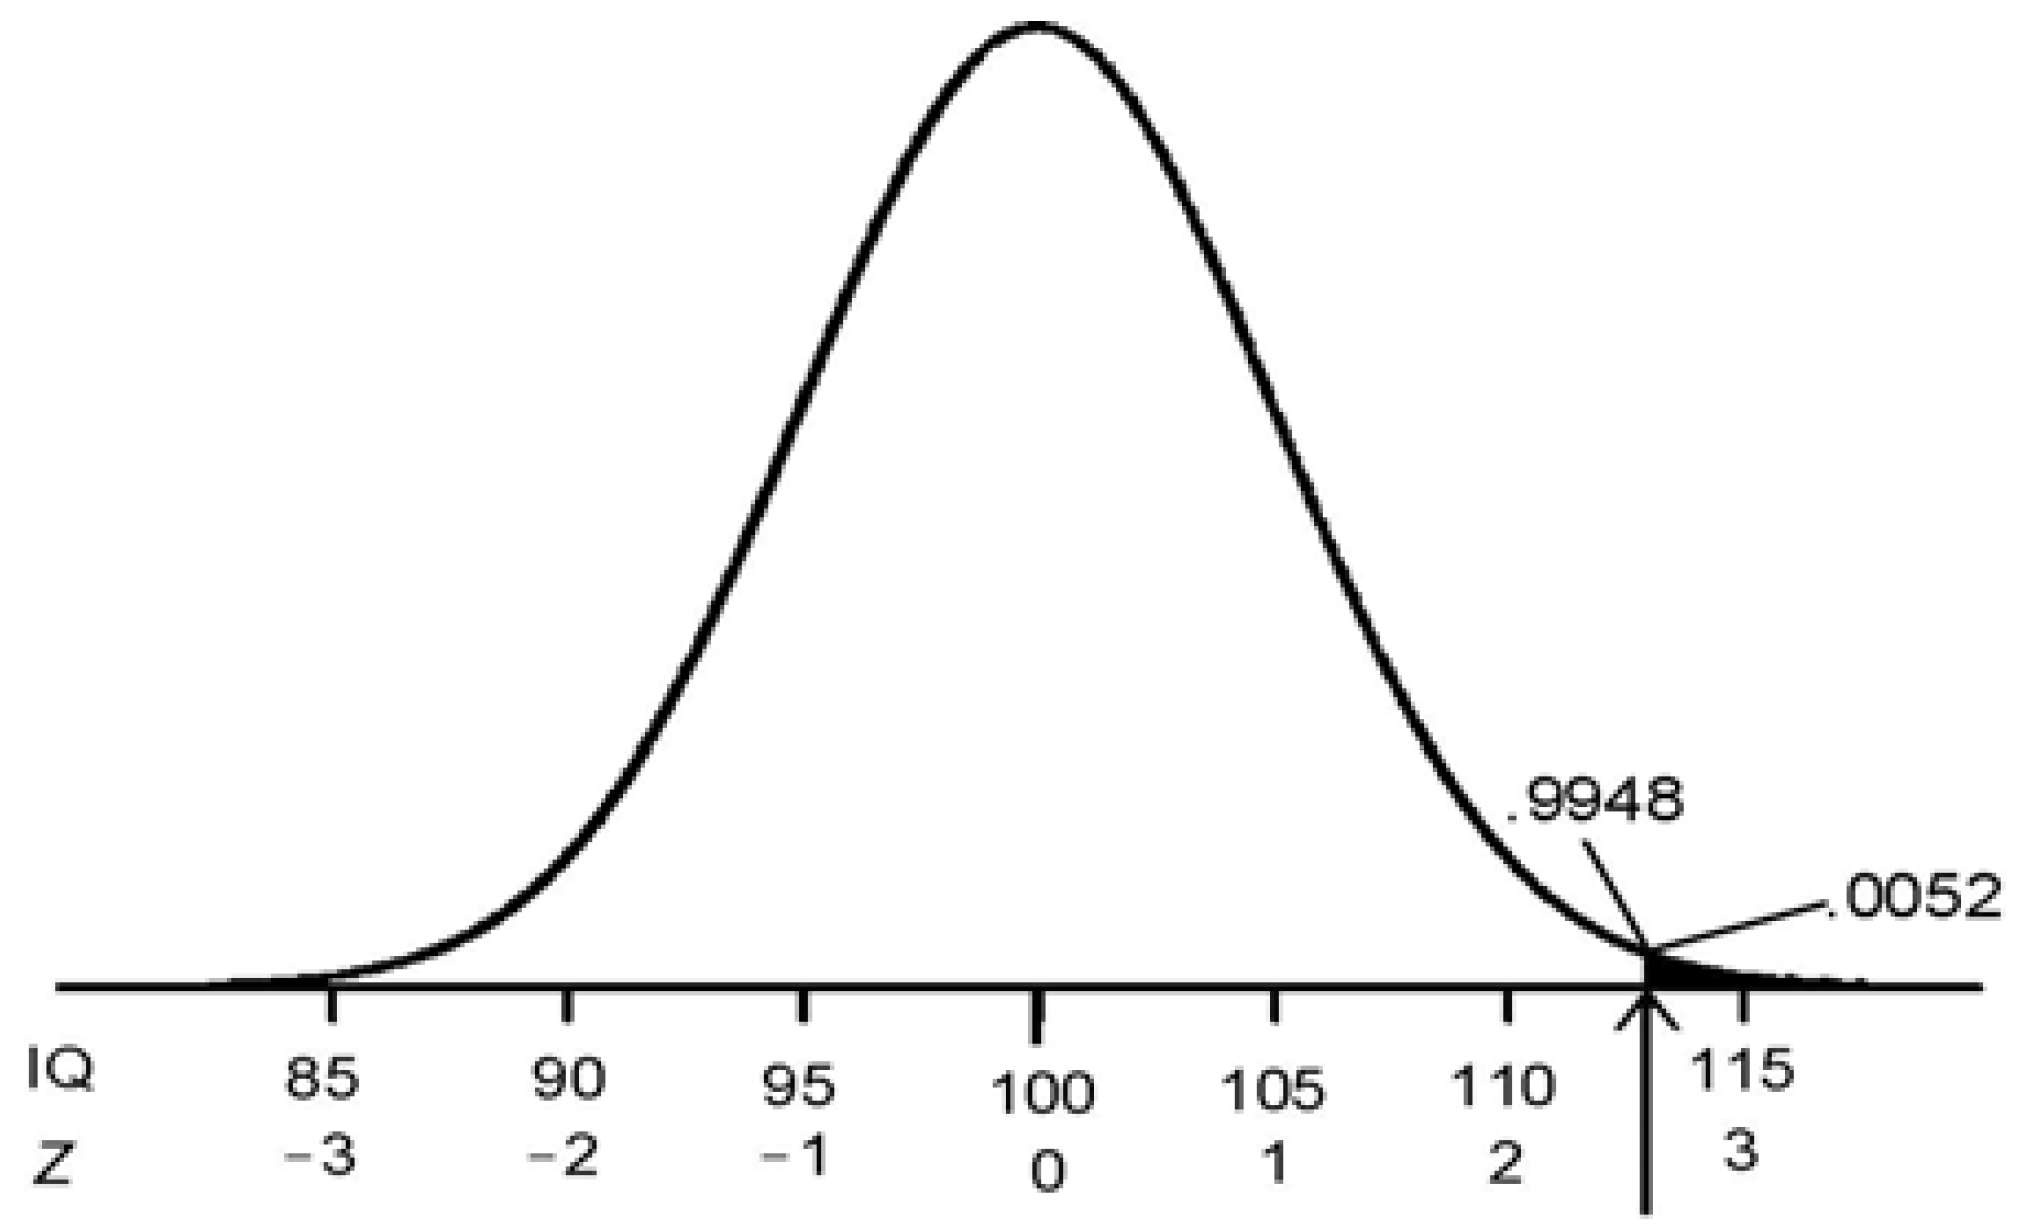
\includegraphics[height=3cm]{images/z_test_2.png}


\pgfmathdeclarefunction{gauss}{2}{%
	\pgfmathparse{1/(#2*sqrt(2*pi))*exp(-((x-#1)^2)/(2*#2^2))}%
}
\tikzstyle{myarrow}=[->, thick]
\begin{tikzpicture}
\begin{axis}[scale=0.525,
no markers, domain=82:118, samples=100,
axis lines*=left, xlabel=$IQ$,axis y line=none,
every axis x label/.style={at=(current axis.right of origin),anchor=west},
every x tick label/.append style={font=\scriptsize, yshift=0.5ex},
height=5cm, width=12cm,label style={font=\tiny},
xtick={80, 85, 90, 95, 100, 105, 110, 115, 120},
xticklabels={$80$, $85$, $90$, $95$, $100$, $105$, $110$, $115$, $120$},
ytick=\empty,
enlargelimits=false, clip=false, axis on top,
x=0.25cm, y=0.25cm/.004,
]
\addplot [fill=black!90, draw=none, domain=112.8:118] {gauss(100,15/sqrt(9))} \closedcycle;
\addplot [fill=black!10, draw=none, domain=82:112.8] {gauss(100,15/sqrt(9))} \closedcycle;
\addplot [thick,cyan!50!black] {gauss(100,15/sqrt(9))};
\coordinate (stat) at (axis cs:112.9,0.0035);
\coordinate (statlabelout) at (axis cs:115,0.0075);
\coordinate (statlabelin) at (axis cs:112,0.0125);
\draw[-, thin] (stat) -- (statlabelout) node[right,font=\tiny]{$.0052$};
\draw[-, thin, black!50] (stat) -- (statlabelin) node[above,font=\tiny]{$.9948$};
\end{axis}

\end{tikzpicture}
\end{center}
\vspace*{-0.2cm}

\begin{itemize}
\item Compare the test statistic (here: $\bar{x}$)\\to its sampling
distribution under $H_0$
\pause 
\medskip
\item \alert{P-value}: probability $p$ of observing values \alert{at least as extreme as $\bar{x}$}\\
%  $\leadsto$ this is the %(computed through cumulative distribution function)
\pause 
\medskip
\item Compare $p$ to pre-defined confidence level $\alpha$ (usually
$\alpha=0.05$);\\\alert{if $p < \alpha$, reject $H_0$}
\pause 
\medskip
\item With $\alpha = 0.01$, would we reject $H_0$ in this case? \hands
\end{itemize}

\end{frame}
%-----------------------------------------------------------------------
%----------------------------------------------------------------------
\begin{frame}[c]{Summary of example}

\begin{itemize}
\item We just used a so-called \alert{$Z$-test}
\item $H_0$: $\mu=\mu_0$, $H_1$: $\mu>\mu_0$  
\item Assumptions: $X \sim \mathcal{N}(\mu,\sigma^2)$ , with known $\mu$ and $\sigma^2$

\medskip
\pause
\item \alert{Test statistic}: sample mean $\bar{x}$; evaluate under 
$\mathcal{N}(\mu=\mu_0,s=\sigma^2/\sqrt{n})$
\pause
\smallskip
\item Equivalent: compute the \alert{Z-statistic}: $Z = (\bar{x}-\mu_0)/s$
and\\
evaluate cumulative density $\Phi(Z)$ of $Z$
under $\mathcal{N}(0,1)$
\medskip
\pause
\begin{itemize}
\item There are standard tables to look up $\Phi(Z)$ for different values of $Z$
\item Nowadays, there are standard libraries to compute $\Phi(Z)$
\end{itemize}

\end{itemize}

\end{frame}
%-----------------------------------------------------------------------
%----------------------------------------------------------------------
\begin{frame}[c]{Two-sided tests}


\vspace*{-0.2cm}
\begin{center}
%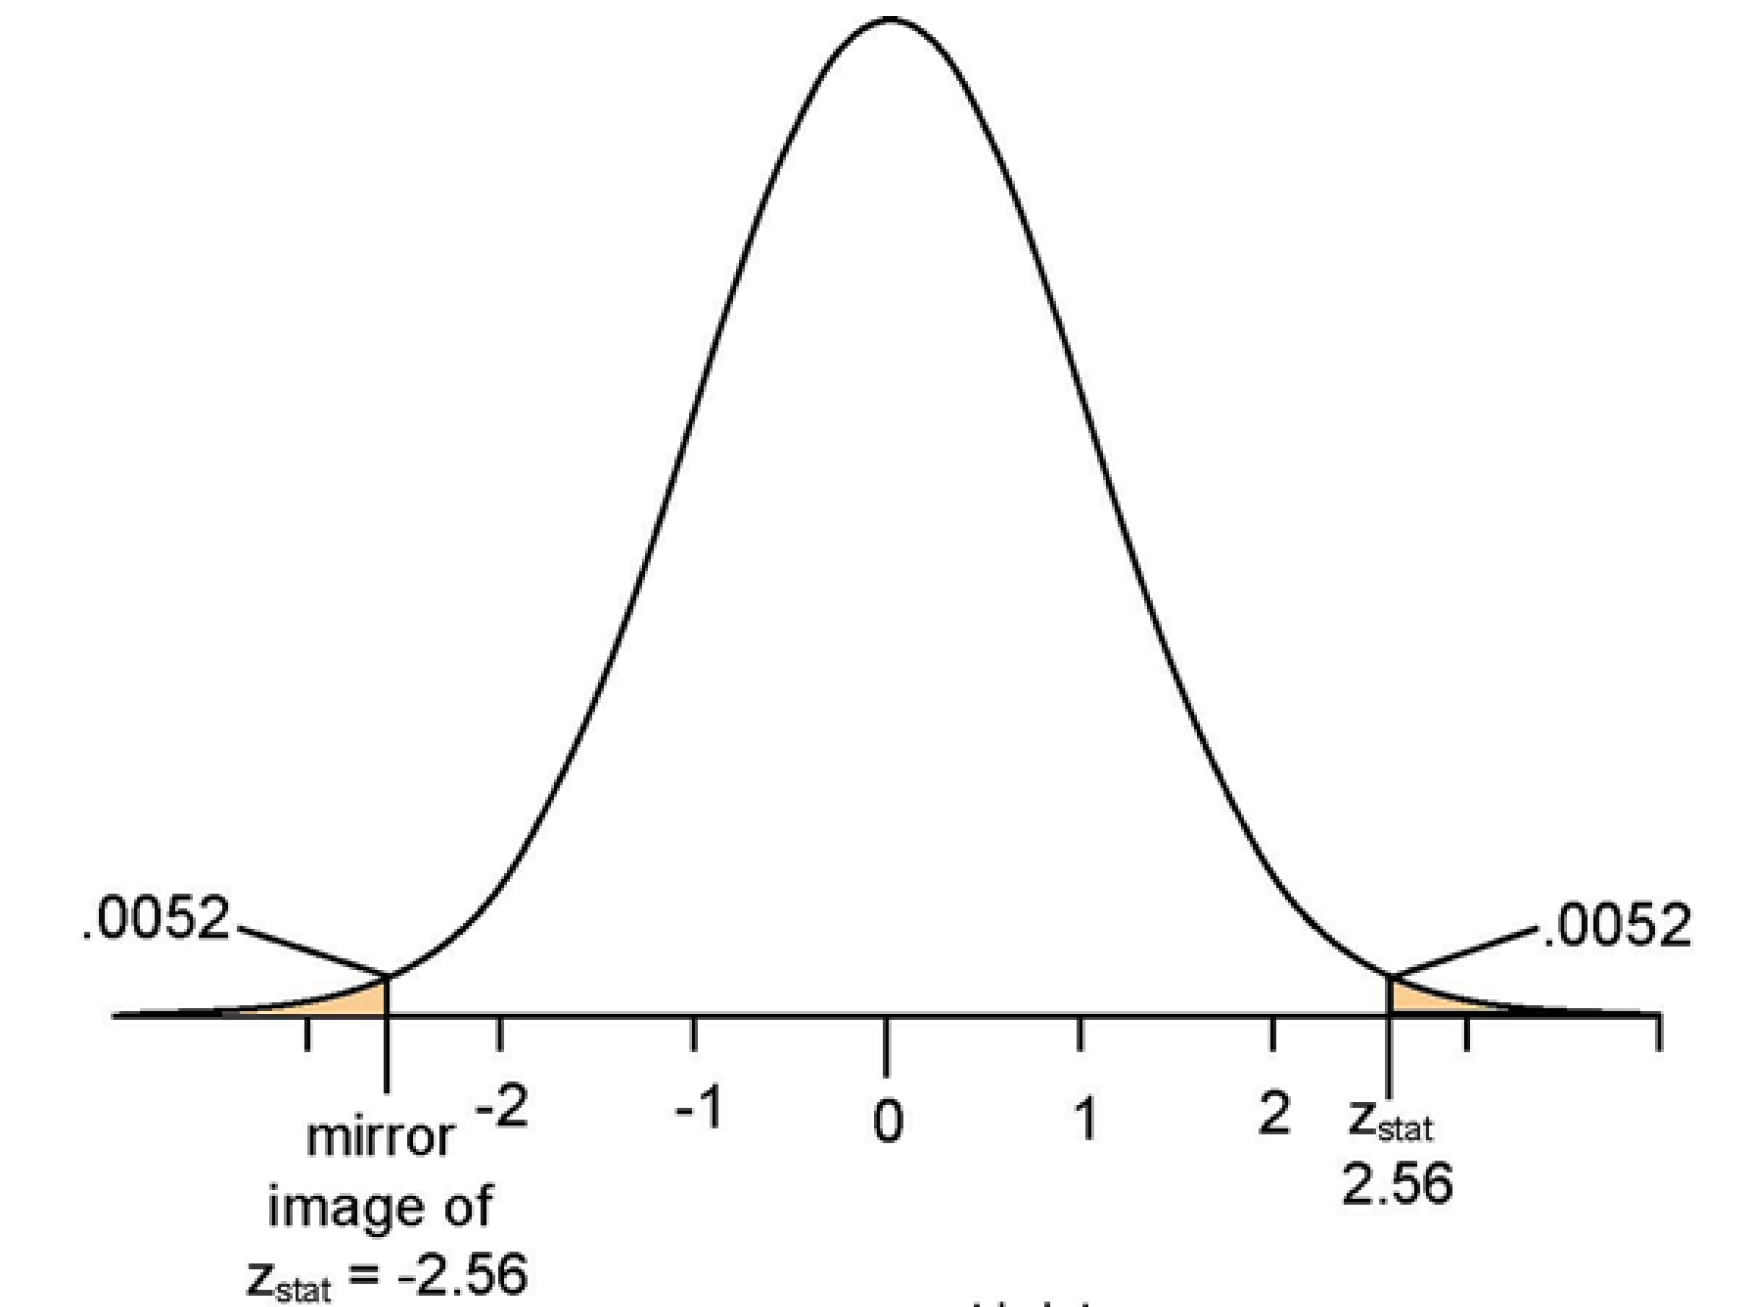
\includegraphics[height=3.5cm]{images/z_test_3.png}


\pgfmathdeclarefunction{gauss}{2}{%
	\pgfmathparse{1/(#2*sqrt(2*pi))*exp(-((x-#1)^2)/(2*#2^2))}%
}
\tikzstyle{myarrow}=[->, thick]
\begin{tikzpicture}
\begin{axis}[scale=0.525,
no markers, domain=82:118, samples=100,
axis lines*=left, xlabel=$IQ$,axis y line=none,
every axis x label/.style={at=(current axis.right of origin),anchor=west},
every x tick label/.append style={font=\scriptsize, yshift=0.5ex},
height=5cm, width=12cm,label style={font=\tiny},
xtick={80, 85, 90, 95, 100, 105, 110, 115, 120},
xticklabels={$80$, $85$, $90$, $95$, $100$, $105$, $110$, $115$, $120$},
ytick=\empty,
enlargelimits=false, clip=false, axis on top,
x=0.25cm, y=0.25cm/.004,
]
\addplot [fill=black!90, draw=none, domain=112.8:118] {gauss(100,15/sqrt(9))} \closedcycle;
\addplot [fill=black!90, draw=none, domain=82:87.2] {gauss(100,15/sqrt(9))} \closedcycle;
%\addplot [fill=black!10, draw=none, domain=82:112.8] {gauss(100,15/sqrt(9))} \closedcycle;
\addplot [thick,cyan!50!black] {gauss(100,15/sqrt(9))};
\coordinate (statright) at (axis cs:112.9,0.0035);
\coordinate (statleft) at (axis cs:87.2,0.0035);
\coordinate (statlabelright) at (axis cs:115,0.0075);
\coordinate (statlabelleft) at (axis cs:85,0.0075);
\draw[-, thin] (statleft) -- (statlabelleft) node[above,font=\tiny]{$.0052$};
\draw[-, thin, black] (statright) -- (statlabelright) node[above,font=\tiny]{$.0052$};
\end{axis}

\end{tikzpicture}
\end{center}
\vspace*{-0.2cm}

\begin{itemize}
\item Similar to one-sided tests, but testing for extreme values in both tails
\item Example Z-test: two-sided alternative hypothesis $H_1$:
$\mu \neq \mu_0$
\pause
\smallskip
\item Compute $Z = (\bar{x}-\mu_0)/s$ as before
\item Compute $p$-value as $p = 2\Phi(Z)$, to account for both tails
\pause 
\medskip
\item With $\alpha = 0.01$, would we reject $H_0$ in this case? \hands
\end{itemize}

\end{frame}
%-----------------------------------------------------------------------
%----------------------------------------------------------------------
\begin{frame}[c]{General points about statistical hypothesis tests}

\begin{itemize}
\item What if $p > \alpha$?
\begin{itemize}
\item \alert{Failure to reject $H_0$}
\item \alert{This does not mean that we accept $H_0$}
\end{itemize}


\pause
\bigskip
\item Beware (i): most tests make some assumptions
\begin{itemize}
\item E.g., $Z$-test and popular $t$-test assume \alert{normality}
\item Our data is often far from normally-distributed
\begin{itemize}
\item[$\leadsto$] E.g., exponential runtime distributions of local search optimizers
\item[$\leadsto$] E.g., distribution of fitting a neural network\\ with different random seeds is not well studied
\end{itemize}
\end{itemize}
\medskip
\pause
\item Beware (ii): if you use cross-validation observations are not independent (you cannot apply statistical tests that assume independence)
%\begin{itemize}
%	\item if you use bootstrap sampling, observations are independent
%\end{itemize}
\end{itemize}

\end{frame}
%-----------------------------------------------------------------------
%----------------------------------------------------------------------
\begin{frame}[c]{The Wilcoxon rank-sum test for non-normal data}

\begin{itemize}
\item Compare the distributions of random variables $X$ and $Y$ 
\begin{itemize}
\item[-] based on samples $x_1, \dots, x_n$ and $y_1, \dots, y_m$
\end{itemize}
\smallskip
\item Assumptions
\begin{itemize}
\item[-] All of $x_1, \dots, x_n$ and $y_1, \dots, y_m$ are independent
from each other 
\item[-] Responses are ordinal (we can compare them)
\end{itemize}  
\pause
\item $H_0$: $P(X > Y) = P(Y > X)$
\pause
\item $H_1$: $P(X > Y) > P(Y > X)$ (one-sided)
\medskip
\pause
\item Test statistic
\begin{itemize}
\item[-] Order all elements $x_i$ and $y_j$ and give them ranks
(1 for smallest)
\item[-] Compute the sum of ranks of $x_i$ and of $y_j$
\smallskip
\pause
\end{itemize}
\item Under $H_0$, the distribution of that test statistic is known\\
$\leadsto$ can evaluate how extreme the observed test statistic is
\end{itemize}

\end{frame}
%-----------------------------------------------------------------------
%----------------------------------------------------------------------
\begin{frame}[c]{The permutation test: another test for non-normal data}

\begin{itemize}
	\item Framework for testing several types of claims
	\item E.g., $H_0$: $X$ and $Y$ have \alert{equal means}
	\item Test statistic: \alert{$t = \frac{1}{n}\sum_{i=1}^n x_i  - 
		\frac{1}{m}\sum_{j=1}^m y_j$}
	\pause
	\medskip
	\item The sampling distribution to compare $t$ against:
	\begin{itemize}
		\item Put $x_1, \dots, x_n$ and $y_1, \dots, y_m$ into a single pool
		\item S = []; repeat, e.g., 10\,000 times
		\begin{itemize}
			\item[-] draw a random permutation \& permute pool with it
			\item[-] add test statistic over permuted pool to $S$
		\end{itemize}
	\end{itemize}
	\pause
	\medskip
	\item $p$-value: percentile of $s$ in $S$:\\
	fraction of samples $s$ in $S$ with $s < t$
	
\end{itemize}

\end{frame}
%-----------------------------------------------------------------------
%----------------------------------------------------------------------
\begin{frame}[c]{Paired vs. unpaired tests}

\begin{itemize}
	\item if you have two unsorted populations (e.g., repeated measurements with different random seeds), you use an unpaired test (as discussed above)
	\item if you can attribute a measurement to concrete objects (e.g., measurements on different datasets), you use a paired test
	\begin{itemize}
		\item paired test are more powerful\\
		(i.e., higher confidence for the same amount of data)
	\end{itemize}
    \item Examples for paired permutation tests
    \begin{itemize}
    	\item Wilcoxon signed rank test
    	\item paired permutation test
    	\begin{itemize}
    		\item permutation of measurement pairs (e.g., same dataset)
    	\end{itemize}
    \end{itemize}
\end{itemize}

\end{frame}
%-----------------------------------------------------------------------
%----------------------------------------------------------------------
\begin{frame}[c]{Multiple Testing Correction}

\begin{itemize}
	\item To compare many systems, we apply statistical tests several time\\
	(once for each pair of systems)
	\item Each test induces some error (bounded by $\alpha$)
	\item[$\leadsto$] the error probability for $k$ tests is bounded by $1 - (1 - \alpha)^k$
	\pause
	\smallskip
	\item Better would be if the error probability would not increase with $k$
	\item[$\leadsto$] multiple testing correction
	\pause
	\smallskip
	\item Bonferronie testing correction: $\alpha_{\text{local}} = \alpha_{\text{global}} / k$
	\pause
	\begin{itemize}
		\item very conservative approach
		\item there exist other, less conservative approaches
	\end{itemize}
	
\end{itemize}

\end{frame}
%-----------------------------------------------------------------------
%----------------------------------------------------------------------
\begin{frame}[c]{Checklist for good scientific practices}

Incomplete list of good scientific practices (specifically for students):
\begin{enumerate}
	\item keep track of your code and design decisions (on all levels)
	\item measure performance of randomized algorithms multiple times\\
		  and show uncertainty of results
	\item apply suitable statistical tests to check for significance
	\item choose a metric that is relevant for the application
	\item always add legends, axis labels and so on in plots
	\item be aware of other research results
	\item avoid peeking at your test data
	\begin{itemize}
		\item no cherry-picking!
	\end{itemize}
\end{enumerate}

\end{frame}
%-----------------------------------------------------------------------
%----------------------------------------------------------------------
\begin{frame}[c]{Learning Goals}

Now, you should be able to \ldots

\begin{itemize}
	\item explain the role of outliers in CS/ML
	\item compare and visualize the performance of different configurations
	\item compare and visualize the performance of AutoML systems
	\item explain and correctly apply statistical hypothesis tests\end{itemize}
\end{frame}
%----------------------------------------------------------------------
%----------------------------------------------------------------------
\begin{frame}[c]{Literature [These are links]}

\begin{itemize}
	\item \lit{\href{https://link.springer.com/content/pdf/10.1023\%2FA\%3A1022623814640.pdf}{P. Langley 1988. Machine Learning as an Experimental Science}}		
    \item \lit{\href{https://www.semanticscholar.org/paper/Machine-Learning-as-an-Experimental-Science-(-)-Drummond/07f052798f17cc761d9e6551c85732e0a41cebb5}{C. Drummod 2006. Machine Learning as an Experimental Science (Revisited)}}	
    \item \lit{\href{http://www.jmlr.org/papers/v7/demsar06a}{J. Demsar 2006. Statistical Comparisons of Classifiers over Multiple Data Sets}}	
    \item \lit{\href{https://journals.plos.org/plosbiology/article?id=10.1371/journal.pbio.1001745}{Wilson et al. 2014. Best Practices for Scientific Computing}}	
    \item \lit{\href{https://journals.plos.org/ploscompbiol/article?id=10.1371/journal.pcbi.1005510}{Wilson et al. 2017. Good enough practices in scientific computing}}
    
    
\end{itemize}

\end{frame}
%----------------------------------------------------------------------

\begin{frame}[c]{}

\centering
\huge
Lecture 4:\\
Hyperparameter optimization\\
Bayesian Optimization
\end{frame}
%----------------------------------------------------------------------
\begin{frame}[c]{Where are we? The big picture}

\begin{itemize}
	\item Introduction
	\item[$\to$] Background
	\begin{itemize}
		\item Design spaces in ML
		\item[$\to$] Evaluation and visualization
	\end{itemize}
	\item Hyperparameter optimization (HPO)
	\begin{itemize}
		\item Bayesian optimization
		\item Other black-box techniques
		\item Speeding up HPO with multi-fidelity optimization
	\end{itemize}
	\item Pentecost (Holiday) -- no lecture
	\item Architecture search I + II
	\item Meta-Learning
	\item Learning to learn $\&$ optimize
	\item Beyond AutoML: algorithm configuration and control
	\item Project announcement and closing
\end{itemize}

\end{frame}
%----------------------------------------------------------------------

%----------------------------------------------------------------------
\begin{frame}[c]{Learning Goals}

After this lecture, you will be able to \ldots

\begin{itemize}
  \item explain the \alert{challenges in hyperparameter optimization}
  \item efficiently optimize black box functions via \alert{Bayesian Optimization}
  \begin{itemize}
    \item discuss the advantages of different \alert{surrogate models}
    \item explain the idea of \alert{acquisition functions} to trade off exploration and exploitation
  \end{itemize}
\end{itemize}


\end{frame}
%-----------------------------------------------------------------------
%----------------------------------------------------------------------
\begin{frame}[c]{How to Optimize Black Box Functions?}

\centering
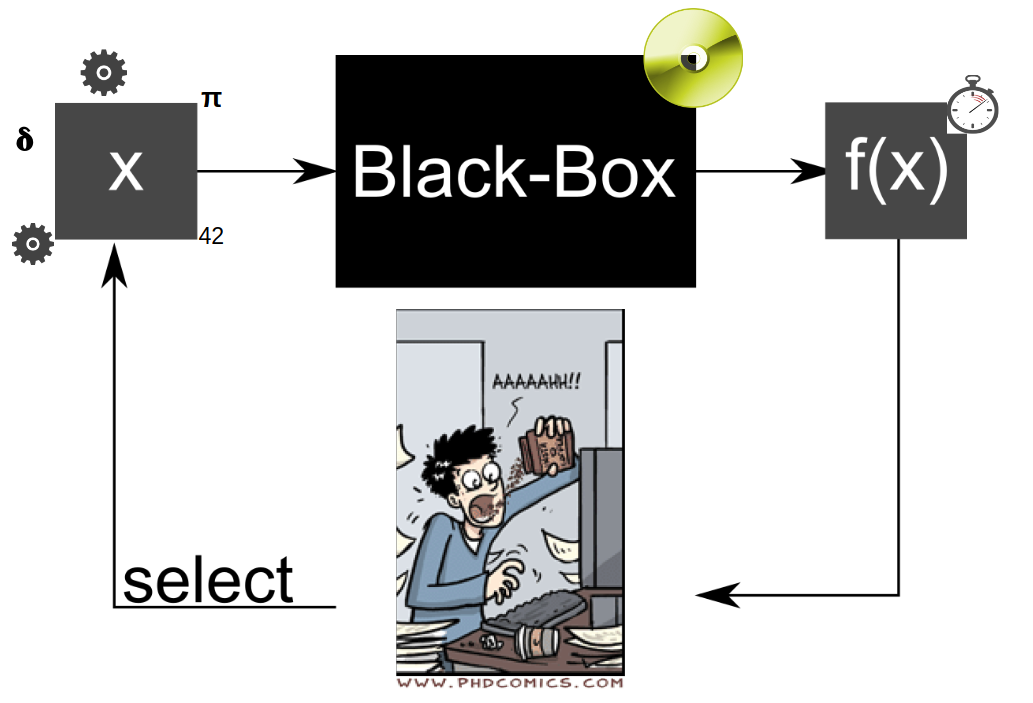
\includegraphics[width=0.7\textwidth]{images/black_box_manual_opt.png}

Only interaction: Query of function at $x$ to obtain $f(x)$

\end{frame}
%-----------------------------------------------------------------------
%----------------------------------------------------------------------
\begin{frame}[c]{How to Optimize Black Box Functions?}

\centering
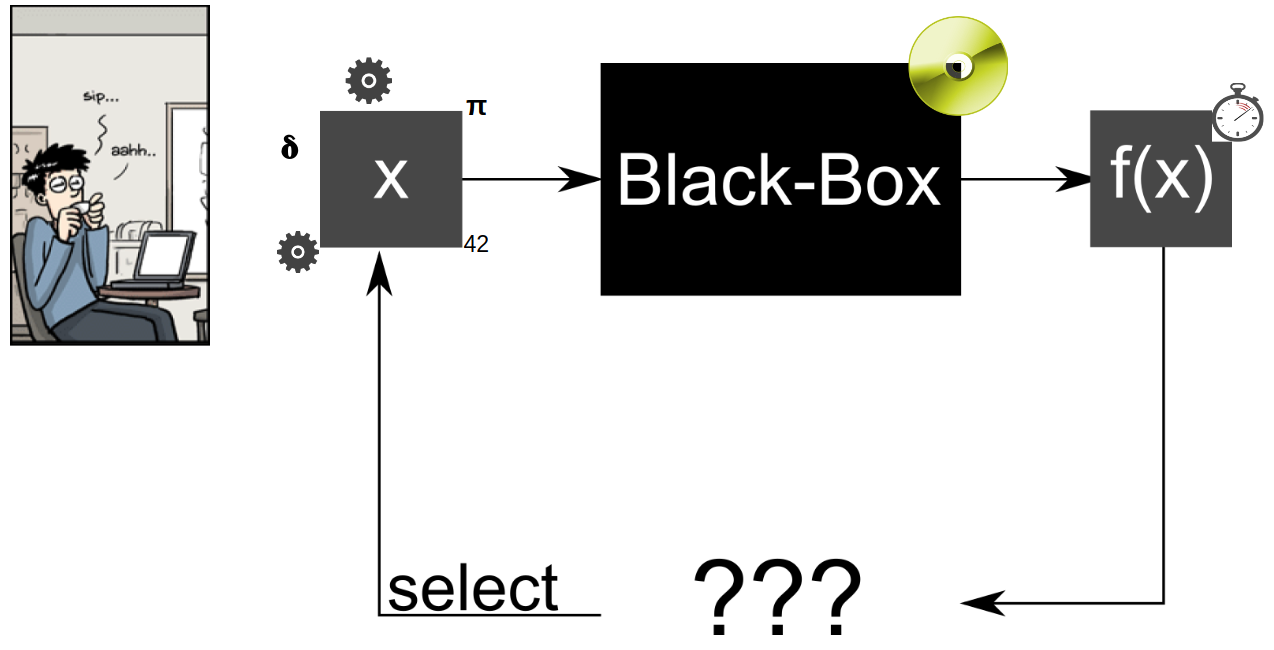
\includegraphics[width=0.9\textwidth]{images/black_box_aut_opt.png}

\end{frame}
%-----------------------------------------------------------------------
%----------------------------------------------------------------------
\begin{frame}[c]{Why Black Box Functions for AutoML?}

\begin{itemize}
  \item Internals of algorithms are often not known\\
  (or well understood)
  \item Extreme: Only way of interaction is running the algorithms
\end{itemize}

\pause
\begin{block}{Example: Hyperparameter Optimization (HPO)}
	Let 
	\begin{itemize}
		\item $\lambda$ be the hyperparameters of an ML algorithm $A$ with domain $\Lambda$,
		\item $D_{opt}$ be a training set which is split into $D_{train}$ and $D_{valid}$ 
		\item $\mathcal{L}(A_\conf, \dataset_{train}, \dataset_{valid})$ denote the loss of $A_\lambda$ trained on $D_{train}$ and evaluated on $D_{valid}$.
	\end{itemize}
	The \emph{hyper-parameter optimization (HPO)} problem is to find a hyper-parameter configuration that minimizes this loss:
	\begin{equation}
	\lambda^* \in \argmin_{\lambda \in \Lambda} \mathcal{L}(A_\conf, \dataset_{train}, \dataset_{valid}) \nonumber  
	\end{equation}
\end{block}

\end{frame}
%----------------------------------------------------------------------
%----------------------------------------------------------------------
\begin{frame}[c]{Challenges in HPO}
\only<1>
{%
	\centering
	
	\vspace*{2.25cm}
	
	What could be challenges in hyperparameter optimization?
	
	\bigskip
	
	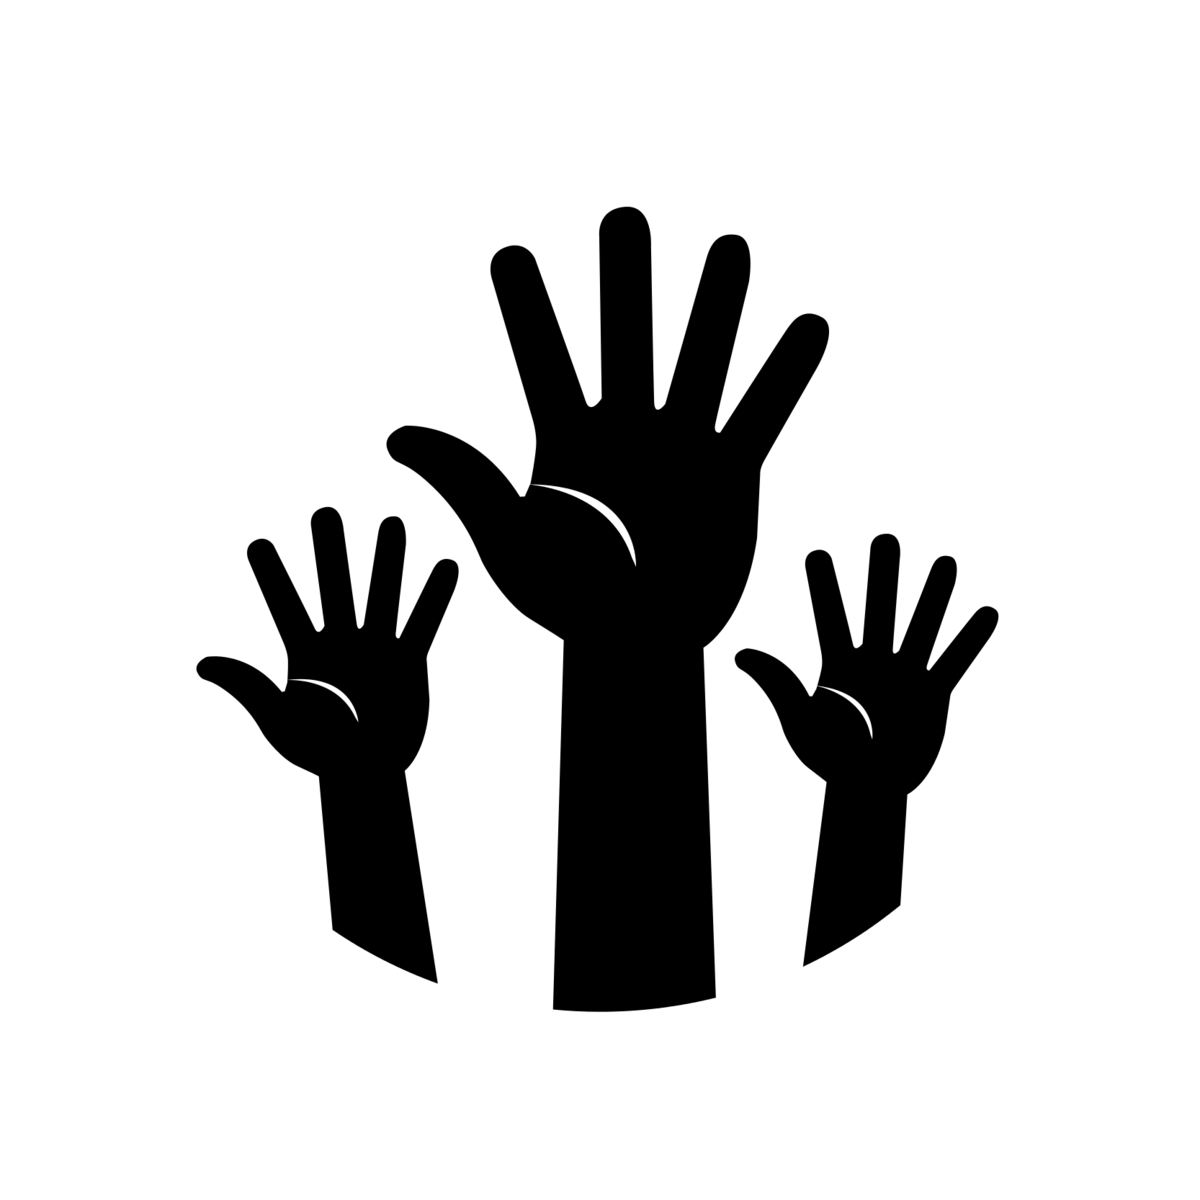
\includegraphics[width=0.2\textwidth]{images/hands.png}
}%
\pause
\begin{itemize}
  \item function evaluations are very expensive
  \begin{itemize}
    \item training a single ML-pipeline can require minutes (or even hours) 
    \item[$\leadsto$] exhaustive search is not feasible
  \end{itemize}
  \pause
  \medskip
  \item complex, structured search space
  \begin{itemize}
    \item small continuous parameter spaces already challenging to optimize
    \item typically, we talk about large configuration spaces\newline ($\gg 10$ hyper-parameters)
    \begin{itemize}
      \item many HPO benchmarks only consider a few continuous parameters
    \end{itemize}
    \item mixed parameter types
    \item conditional structures
  \end{itemize}
  \pause
  \medskip
  \item resembles a black-box optimization problem
  \begin{itemize}
    \item Input: hyperparameter configuration
    \item Black box: ML pipeline 
    \item Output: loss
    \item Note: no gradient information available
  \end{itemize}
\end{itemize}

\end{frame}
%----------------------------------------------------------------------
\begin{frame}[c]{How to Optimize Black Box Functions?}

\centering
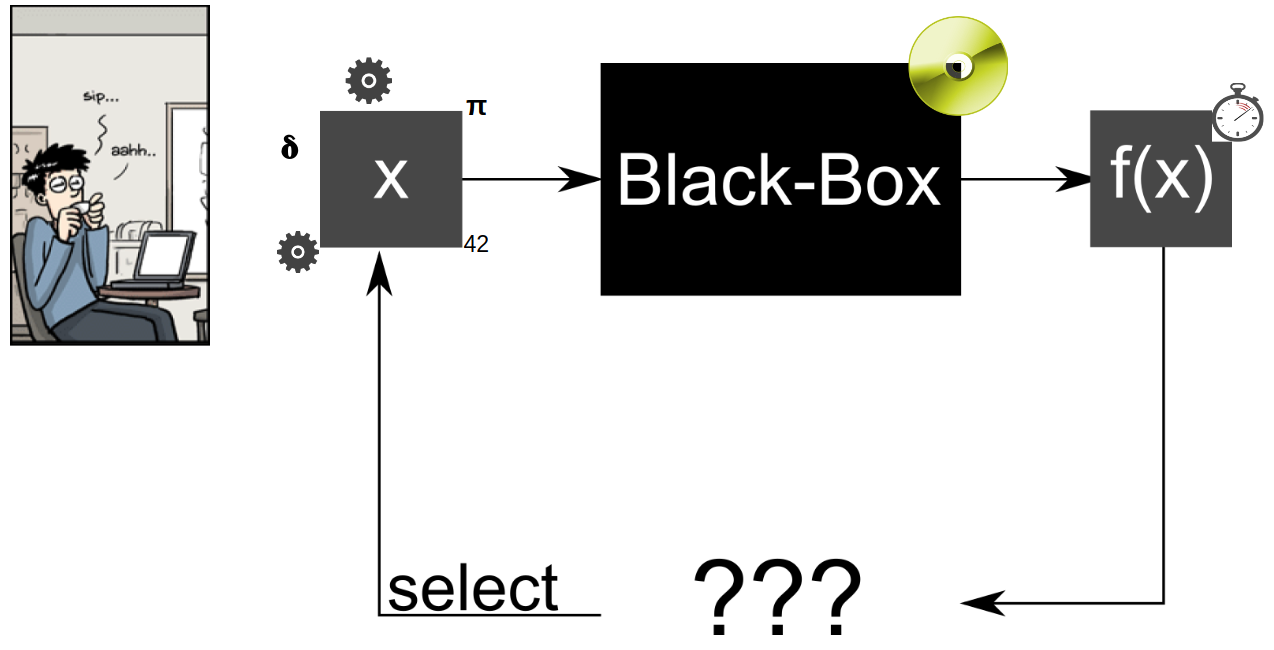
\includegraphics[width=0.9\textwidth]{images/black_box_aut_opt.png}

\end{frame}
%-----------------------------------------------------------------------
%-----------------------------------------------------------------------
\begin{frame}[c,fragile]{Grid Search \litw{Bergstra et al. '12}}

\begin{center}
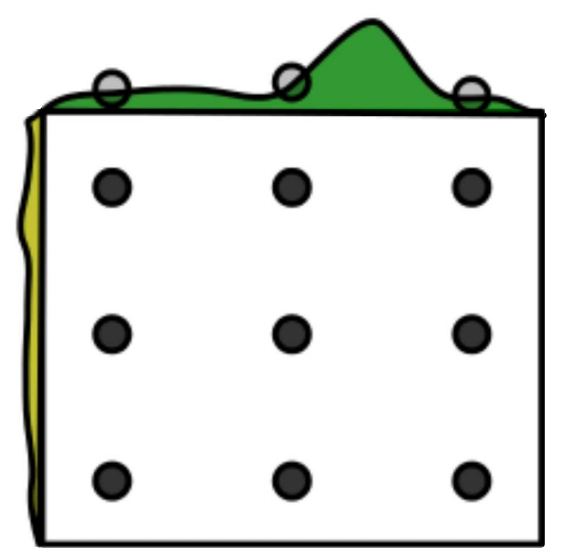
\includegraphics[width=0.28\textwidth]{images/grid_search}%
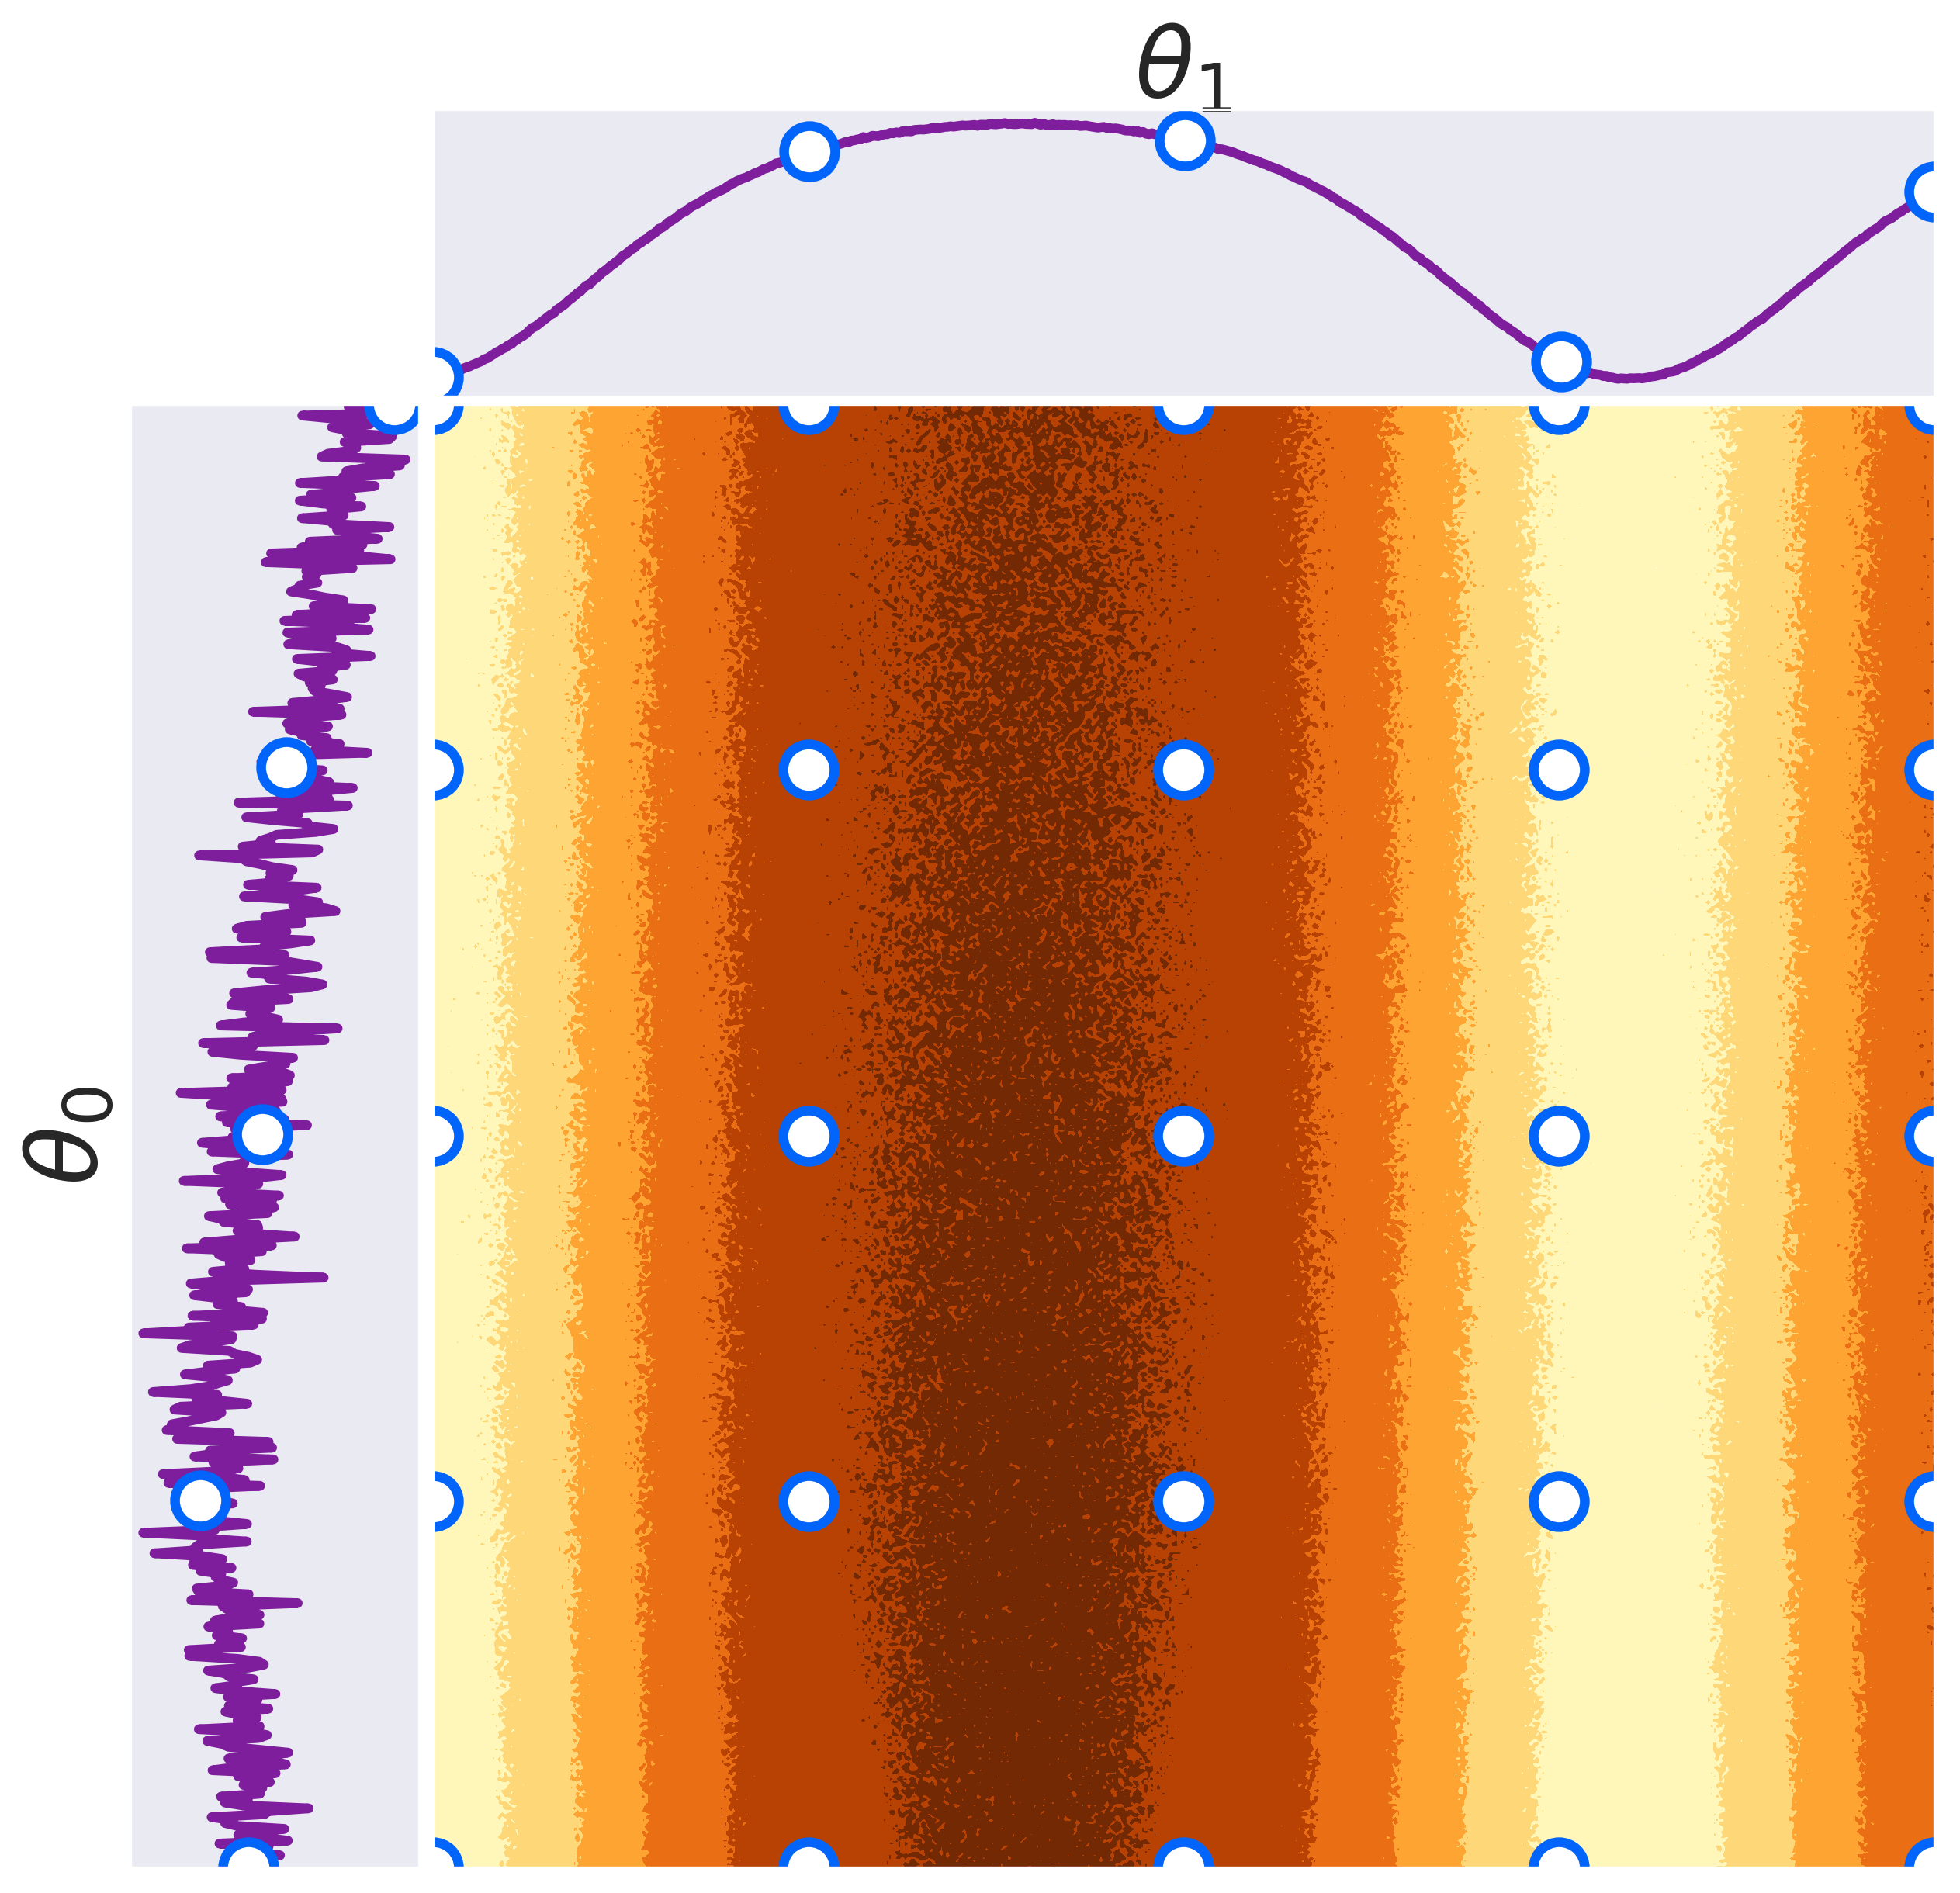
\includegraphics[width=0.28\textwidth]{images/gs}
\end{center}

\begin{block}{Pros and Cons}

\only<1-2>{\hands What are potential pros and cons of grid search?}
\pause

\begin{columns}
\column{0.4\textwidth}
Pros:
\begin{itemize}
  \item easy to implement
  \item easy to parallelize 
\end{itemize}

\column{0.6\textwidth}
Cons:
\begin{itemize}
  \item discretization of $\pcs$?
  \item does not scale with $\#$hyperparameters
  \item inefficient if not all hyperparameters are important
\end{itemize}


\end{columns}

\end{block}

\end{frame}
%-----------------------------------------------------------------------
%-----------------------------------------------------------------------
\begin{frame}[c,fragile]{Random Search \litw{Bergstra et al. '12}}

\begin{center}
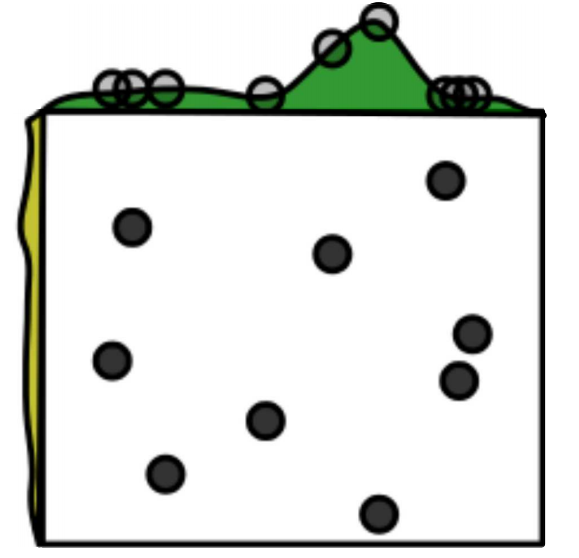
\includegraphics[width=0.28\textwidth]{images/random_search}%
\includegraphics[width=0.28\textwidth]{images/rs}
\end{center}

\begin{block}{Pros and Cons}

\only<1-2>{\hands What are potential pros and cons of random search?}
\pause

\begin{columns}
\column{0.4\textwidth}
Pros:
\begin{itemize}
  \item even easier to implement
  \item easy to parallelize 
  \item more evaluations along each parameter
\end{itemize}

\column{0.6\textwidth}
Cons:
\begin{itemize}
  \item does not scale with $\#$hyper-parameters
  \item purely explorative
\end{itemize}


\end{columns}

\end{block}

\end{frame}
%-----------------------------------------------------------------------

%-----------------------------------------------------------------------
\begin{frame}[c,fragile]{Optimization for HPO}

\begin{itemize}
	\item HPO is expensive $\leadsto$ we need also a greedy optimization approach
	\item basically, all black-box optimization approaches could be used
	\begin{itemize}
		\item Local search
		\begin{itemize}
			\item hypothesis: HPO surfaces have many local optima s.t. local search gets easily trapped in local optima
		\end{itemize}
	 	\medskip
		\item population-based evolution strategies (more next week)
		\begin{itemize}
			\item often needs many function evaluations to perform well
		\end{itemize}
		\medskip
		\item model-based approaches
		\begin{itemize}
			\item Idea: use an surrogate model to approximate the unknown function to be optimized
		\end{itemize}
	    \item Remark: there are also combinations of these approaches (such as model-based ES)
	\end{itemize}
\end{itemize}

\end{frame}
%-----------------------------------------------------------------------
%-----------------------------------------------------------------------
\begin{frame}[c,fragile]{Model-based Optimization \litw{Bergstra et al. 2011}}

\begin{itemize}
	\item Assume that we already observed some configuration and the corresponding loss $D = \{(\conf_i, y_i))\}_{i=1}^N$
	\begin{itemize}
		\item let's use $y_i = f(\lambda)$ as a short form for $\loss(\algo_\conf, \dataset_{train}, \dataset_{valid})$
	\end{itemize}
	\item We could approximate the good region of the configuration space $\pcs$
\end{itemize}

$$
p(x|y) = \begin{cases}
l(x) \text{ if } y < y^*\\
g(x) \text{ otherwise} 
\end{cases}
$$

where 
\begin{itemize}
	\item $y^*$ is an empirical threshold for a well-performing configuration (e.g., a $\gamma$ percentile of all observed $y$ in $D$)
	\item $l(x)$ models the density of the well-performing region based on $D$
	\begin{itemize}
		\item Note that we minimize!
	\end{itemize}
	\item $g(x)$ models the density of the poorly performing region based on $D$
	\item $g$ and $l$ can be modeled by kernel density estimator (KDE)
\end{itemize}

\end{frame}
%-----------------------------------------------------------------------
%-----------------------------------------------------------------------
\begin{frame}[c,fragile]{Model-based Optimization \litw{Bergstra et al. 2011}}

UPDATE!

\begin{algorithm}[H]
	\Input{Search Space $\mathcal{X}$,
		black box function $f$, 
		acquisition function $\alpha$,
		maximal number of function evaluations $m$
	}
	\BlankLine
	$\mathcal{D}_0$ $\leftarrow$ initial\_design($\mathcal{X}$); \\
	\For{n = $1, 2, \ldots m - |D_0|$}{
		%\While{$B$ not exhausted} {
		$\surro$ $\leftarrow$ fit predictive model on $\mathcal{D}_{n-1}$;\\
		select $x_{n}$ by optimizing $x_{n} \in \argmax_{x \in \mathcal{X}} \alpha(x; \mathcal{D}_{n-1}, \surro)$;\\
		Query $y_{n} := f(x_{n})$;\\
		Add observation to data $D_{n} := D_{n-1} \cup \{\langle x_{n}, y_{n} \rangle \}$;\\
	}
	\Return{Best $x$ according to $D_m$ or $\surro$}
	\caption{Bayesian Optimization (BO)}
\end{algorithm}


\end{frame}
%-----------------------------------------------------------------------
%-----------------------------------------------------------------------
\begin{frame}[c,fragile]{Bayesian Optimization \litw{J. Mockus 1977, D .Jones et al. 1998}}

\begin{columns}

\column{0.4\textwidth}

\includegraphics[width=\textwidth]{images/bo_pic1.png}\\
\pause
\includegraphics[width=\textwidth]{images/bo_pic2.png}\\
\pause
\includegraphics[width=\textwidth]{images/bo_pic3.png}
\pause

\column{0.55\textwidth}
General Approach:
\begin{enumerate}
  \item Fit model on collected observations $\langle{}\conf, f(\conf)\rangle{}$
  \pause
  \item use acquisition function $a$ to trade off exploration and exploitation
  \pause
  \item maximize acquisition function: $x^* \in \argmin a(x)$
  \pause
  \item obtain new observation at $x^*$
\end{enumerate}

\pause
Moving pieces:
\begin{itemize}
  	\item Which \alert{model family} to use 
	\item How to use the model to guide optimization
	\begin{itemize}
		\item Determined by $a(x)$\\
		(Which data point should I \emph{acquire} next?) 
	\end{itemize}
\end{itemize}

\end{columns}

\end{frame}
%-----------------------------------------------------------------------
%-----------------------------------------------------------------------
\begin{frame}[c,fragile]{Bayesian Optimization: Algorithm}

\begin{algorithm}[H]
	\Input{Search Space $\mathcal{X}$,
		black box function $f$, 
		acquisition function $\alpha$,
		maximal number of function evaluations $m$
	}
	\BlankLine
	$\mathcal{D}_0$ $\leftarrow$ initial\_design($\mathcal{X}$); \\
	\For{n = $1, 2, \ldots m - |D_0|$}{
		%\While{$B$ not exhausted} {
		$\surro$ $\leftarrow$ fit predictive model on $\mathcal{D}_{n-1}$;\\
		select $x_{n}$ by optimizing $x_{n} \in \argmax_{x \in \mathcal{X}} \alpha(x; \mathcal{D}_{n-1}, \surro)$;\\
		Query $y_{n} := f(x_{n})$;\\
		Add observation to data $D_{n} := D_{n-1} \cup \{\langle x_{n}, y_{n} \rangle \}$;\\
	}
	\Return{Best $x$ according to $D_m$ or $\surro$}
	\caption{Bayesian Optimization (BO)}
\end{algorithm}


\end{frame}
%-----------------------------------------------------------------------
%-----------------------------------------------------------------------
\begin{frame}[c,fragile]{Bayesian Optimization}

\begin{block}{Pros and Cons}

Pros:
\begin{itemize}
  \item sample efficient
  \item can be applied to many black-box functions with expensive function evaluations (not only HPO)
\end{itemize}

Cons:
\begin{itemize}
  \item overhead because of model training in each iteration
  \item hard to efficiently parallelize
  \item (requires good surrogate model)
\end{itemize}

\end{block}

\end{frame}
%-----------------------------------------------------------------------


%%%%%%%%%%%%%%%%%%%%%%%%%%%%%%%%%%%%%%%%%%%%%%%%%%%%%%%%%%%%%%%%%%%%%%%%%
\begin{frame}[c,fragile]{The Role of the Acquisition Function}
\begin{itemize}
  \item Given: a model $\hat{f}:\confs \rightarrow \mathds{R}$ that predicts the quality $\mu(\conf)$ for each configuration $\conf$ and its standard deviation $\sigma(\conf)$ ($\leadsto$ uncertainty)
  \begin{itemize}
  	\item Assume w.l.o.g. that we want to \emph{maximize} $f$
  \end{itemize}
  \medskip
  \pause
  \item Which configuration should we select next? Need to trade off: 
  \begin{itemize}
    \item \alert{Exploitation}\\(sampling where the predicted mean $\mu(\conf)$ is high)
    \item \alert{Exploration}\\(sampling where we're uncertain about f; i.e., $\sigma(\conf)$ is high)
  \end{itemize}
  \medskip
  \pause
  \item Various acquisition functions achieve this trade-off
\end{itemize}

\end{frame}
%%%%%%%%%%%%%%%%%%%%%%%%%%%%%%%%%%%%%%%%%%%%%%%%%%%%%%%%%%%%%%%%%%%%%%%%%


%%%%%%%%%%%%%%%%%%%%%%%%%%%%%%%%%%%%%%%%%%%%%%%%%%%%%%%%%%%%%%%%%%%%%%%%%
\begin{frame}[c,fragile]{Probability of Improvement}
\begin{itemize}
\vspace*{-0.2cm}
  \item Let $f(\theta^+)$ denote the best (here: max) function value known so far.
\vspace*{-0.2cm}  
  \begin{eqnarray}
\nonumber{}  PI(\conf) & = & P(f(\conf) \ge f(\theta^+))) = \Phi \left( \frac{\mu(\theta) - f(\theta^+)}{\sigma(\theta)} \right)
  \end{eqnarray}
  \item Here, $\Phi$ is the cumulative distribution function of the standard normal distribution. (There are $\mathcal{O}(1)$ lookup tables for this.)
\end{itemize}
\centering
\includegraphics[width=0.55\textwidth]{images/Acquisition-PI.png} 

\end{frame}
%%%%%%%%%%%%%%%%%%%%%%%%%%%%%%%%%%%%%%%%%%%%%%%%%%%%%%%%%%%%%%%%%%%%%%%%%

%%%%%%%%%%%%%%%%%%%%%%%%%%%%%%%%%%%%%%%%%%%%%%%%%%%%%%%%%%%%%%%%%%%%%%%%%
\begin{frame}[c,fragile]{Expected Improvement}

\begin{itemize}
\vspace*{-0.2cm}
  \item Like probability of improvement, but also takes into account the \alert{magnitude} of the improvement.
  \item Define the improvement at a point $\conf$ as:\\
\vspace*{-0.2cm}
  \begin{equation}
  \nonumber{}I(\conf) = \max (f(\conf) - f(\conf^+), 0)
  \end{equation}
  \pause
\vspace*{-0.4cm}  
  \item Then, we can compute the expectation of this improvement across the predictive distribution
  \begin{eqnarray}
\nonumber{} \mathds{E}[I(x)] = \int_{-\infty}^{\infty} \max (f(\conf) - f(\conf^+), 0) \cdot \norm( f(\conf) ; \mu(\conf), \sigma^2(\conf) )  df(\conf) 
  \end{eqnarray}
  \pause
\vspace*{-0.2cm}
  \item This turns out to have a closed form solution:
  \small
  \begin{eqnarray}
\nonumber{} \mathds{E}[I(x)] = (\mu(\conf) - f^+) \Phi\left( \frac{\mu(\conf) - f(\conf^+)}{\sigma(\conf)} \right)  + \sigma(\conf) \phi \left( \frac{\mu(\conf) - f(\conf^+)}{\sigma(\conf)} \right)
  \end{eqnarray}
\end{itemize}

\end{frame}
%%%%%%%%%%%%%%%%%%%%%%%%%%%%%%%%%%%%%%%%%%%%%%%%%%%%%%%%%%%%%%%%%%%%%%%%%

%%%%%%%%%%%%%%%%%%%%%%%%%%%%%%%%%%%%%%%%%%%%%%%%%%%%%%%%%%%%%%%%%%%%%%%%%
\begin{frame}[c,fragile]{Upper Confidence Bound}
\begin{itemize}
\vspace*{-0.2cm}
  \item UCB$(\conf) = \mu(\conf) + \kappa\sigma(\conf)$, with exploration parameter $\kappa$
\end{itemize}
\vspace*{-0.2cm}  
\centering
\includegraphics[width=0.55\textwidth]{images/Acquisition-UCB.png} 
\vspace*{0.2cm}  
\begin{itemize}
\item Which point would we pick next with UCB and $\kappa = 1$? \hands
\pause
 \item GP-UCB$(\conf) = \mu(\conf) + \sqrt{\beta_t} \sigma(\conf)$, with $\beta_t$ \alert{increasing} over time\\
 \lit{Srinivas et al. 2009}
\end{itemize}

\end{frame}
%%%%%%%%%%%%%%%%%%%%%%%%%%%%%%%%%%%%%%%%%%%%%%%%%%%%%%%%%%%%%%%%%%%%%%%%%
%%%%%%%%%%%%%%%%%%%%%%%%%%%%%%%%%%%%%%%%%%%%%%%%%%%%%%%%%%%%%%%%%%%%%%%%%
\begin{frame}[c,fragile]{Entropy Search}

TODO

\end{frame}
%%%%%%%%%%%%%%%%%%%%%%%%%%%%%%%%%%%%%%%%%%%%%%%%%%%%%%%%%%%%%%%%%%%%%%%%%

%%%%%%%%%%%%%%%%%%%%%%%%%%%%%%%%%%%%%%%%%%%%%%%%%%%%%%%%%%%%%%%%%%%%%%%%%
\begin{frame}[c,fragile]{Surrograte model Model}

Required features

\begin{itemize}
  \item Mandatory:
  \begin{itemize}
    \item Regression model
	\item Uncertainty estimates
  \end{itemize}
  \pause
  \item Preferable:
  \begin{itemize}
    \item accurate predictions
    \item cheap-to-train
    \item scales with the complexity of the data\\ (number of features and observations)
    \item can handle different types of features\\ (categorical and continuous)
  \end{itemize}
\end{itemize}

\pause
Common choice: Gaussian Processes\\
Our choice: Random Forests

\end{frame}
%%%%%%%%%%%%%%%%%%%%%%%%%%%%%%%%%%%%%%%%%%%%%%%%%%%%%%%%%%%%%%%%%%%%%%%%%

%%%%%%%%%%%%%%%%%%%%%%%%%%%%%%%%%%%%%%%%%%%%%%%%%%%%%%%%%%%%%%%%%%%%%%%%%
\begin{frame}[c,fragile]{Recap Random Forests}


\centering
\includegraphics[width=0.55\textwidth]{images/random_forest_pic}

\begin{itemize}
  \item Train:
  \begin{itemize}
    \item $n$ decision (or regression) trees (potentially with pruning)
    \item subsampled training data for each tree (with bootstrapping)
    \item subsampled feature set for each split
  \end{itemize}
  \item Predict
  \begin{itemize}
    \item Obtain prediction of each tree
    \item Aggregate predictions (voting, average, \ldots)
    \pause
    \item Uncertainty predictions: average across tree predictions 
  \end{itemize}
\end{itemize}


\end{frame}
%%%%%%%%%%%%%%%%%%%%%%%%%%%%%%%%%%%%%%%%%%%%%%%%%%%%%%%%%%%%%%%%%%%%%%%%%
%%%%%%%%%%%%%%%%%%%%%%%%%%%%%%%%%%%%%%%%%%%%%%%%%%%%%%%%%%%%%%%%%%%%%%%%%
\begin{frame}[c,fragile]{Advantages and Disadvantages of Random Forests}


\begin{columns}
\column{0.5\textwidth}
Pros:
\begin{itemize}
  \item Cheap to train
  \item Scales well with \#observations
  \begin{itemize}
    \item Worst-case complexity for $T$ tress with $n$ data points of dimensionality $p$: $\mathcal O(T\cdot p \cdot n^2 \log{n})$
  \end{itemize}
  \item training can be parallelized
  \item Can handle continuous and categorical features
  \begin{itemize}
    \item most RF implementations can handle only continuous features
  \end{itemize}
\end{itemize}

\column{0.5\textwidth}
Cons:
\begin{itemize}
  \item Poor uncertainty estimates
  \item No extrapolation
  \begin{itemize}
    \item last seen value for extrapolation (constant)
  \end{itemize}
\end{itemize}

\end{columns}

\end{frame}
%%%%%%%%%%%%%%%%%%%%%%%%%%%%%%%%%%%%%%%%%%%%%%%%%%%%%%%%%%%%%%%%%%%%%%%%%
%----------------------------------------------------------------------
\begin{frame}[c]{Preprocessing Configuration}

\begin{block}{Convert $\conf$ for ML Model}
  \begin{itemize}
    \item continuous and integer parameter can be directly passed
    \begin{itemize}
      \item scaled to $[0,1]$
    \end{itemize}
    \pause
    \item categorical parameters should be encoded if necessary
    \begin{itemize}
      \item e.$\,$g., random forest can handle categorical parameter natively\\
      (Not all implementations are able to do it!) 
      \item use one-hot encoding if necessary:
      \begin{itemize}
        \item add new variable for each possible value $v_i$
        \item set one of these variable to one (depending on the configuration)
      \end{itemize}
    \end{itemize}
    \pause
    \item ordinal parameters can be converted to integers or also one-hot encoded
  \end{itemize}
\end{block}


\end{frame}
%-----------------------------------------------------------------------
%----------------------------------------------------------------------
\begin{frame}[c]{Preprocessing Configuration (cont'd)}

\begin{block}{Conditional Hyperparameters}
  \begin{itemize}
    \item Configuration spaces often have a hierarchical structure
    \item e.$\,$g., hyperparameter A is only active if heuristic H is used
    \pause
    \item[$\leadsto$] List of hyperparameter values has missing entries because of inactive hyperparameters
    \medskip
    \pause
    \item Fixes:
    \begin{itemize}
    	\item Impute missing data, e.$\,$g., by default setting
    	\item Mark these inactive hyperparameters and let the model deal with it\\
    		  e.$\,$g., a random forest could only split on active parameters
    \end{itemize}
  \end{itemize}
\end{block}

\end{frame}
%-----------------------------------------------------------------------
{\setbeamertemplate{logo}{}
\begin{frame}[c,fragile]{Important Design Dimensions in BO}

\only<1>{
\begin{block}{Transformation of y-values}
	\begin{minipage}{0.6\textwidth}
		\begin{figure}[H]
			\centering
			\includegraphics[height=.6\textheight]{images/borf_boxplot_y}
		\end{figure}
	\end{minipage} \hfill
	\begin{minipage}{0.39\textwidth}
		\begin{itemize}
			\item log-transformed values to fit the model and the acquisition function improves performance
			\item less emphasize on large outlier values
			\item focus more on small improvements and less on exploration in unexplored spaces
		\end{itemize}
	\end{minipage}
\end{block}
}

\only<2>{
	\begin{block}{Interleaving Random Points}
		\begin{minipage}{0.6\textwidth}
			\begin{figure}[H]
				\centering
				\includegraphics[height=.6\textheight]{images/borf_boxplot_r}
			\end{figure}
		\end{minipage} \hfill
		\begin{minipage}{0.39\textwidth}
			\begin{itemize}
				\item RFs don't extrapolate well
				\item Interpolation between two observations with similar function values leads to
				constant uncertainty estimates
				\item BO with RFs can easily get stuck in local optima
				\item interleave randomly sampled points to escape local optima
			\end{itemize}
		\end{minipage}
	\end{block}
}

\only<3>{
	\begin{block}{Initial Design}
		\begin{minipage}{0.6\textwidth}
			\begin{figure}[H]
				\centering
				\includegraphics[height=.6\textheight]{images/borf_boxplot_init}
			\end{figure}
		\end{minipage} \hfill
		\begin{minipage}{0.39\textwidth}
			\begin{itemize}
				\item Alternative to exploration via randomly sampled points
				\item explore the space before the actual BO takes place
				\item Pro: will improve the EPM in early iterations
				\item Con: will invest a considerable number of function evaluations without taking the already gathered knowledge into account
			\end{itemize}
		\end{minipage}
	\end{block}
}
\end{frame}
}
%----------------------------------------------------------------------
\begin{frame}[c]{Learning Goals}

After this lecture, you are able to \ldots

\begin{itemize}
	\item explain the \alert{challenges in hyperparameter optimization}
	\item efficiently optimize black box functions via \alert{Bayesian Optimization}
	\begin{itemize}
		\item discuss the advantages of different \alert{surrogate models}
		\item explain the idea of \alert{acquisition functions} to trade off exploration and exploitation
	\end{itemize}
	\item define \alert{configuration spaces}
	\item understand \alert{grey-boxes} for hyperparameter optimization (HPO)
\end{itemize}
\end{frame}
%-----------------------------------------------------------------------
%\input{lecture5-es+hpo.tex}
%%-----------------------------------------------------------------------
\begin{frame}[c,fragile]{What if a single configuration is too expensive?}


\begin{itemize}
  \item Sometimes, even validating a single configuration needs a lot of time\\
  		e.$\,$g., single function evaluation takes hours or even days:
  \begin{itemize}
    \item ML on big data
    \item Training a deep neural network  
  \end{itemize}
  \pause
  \item Challenge: We cannot search for a configuration if we can afford very few function evaluations $< 10$
  \pause
  \item \hands What could we do?
  \pause
  \begin{itemize}
    \item Data subset selection
    \item Predict learning curves
  \end{itemize}
  \item[$\leadsto$] Going from black-box to grey-box optimization
\end{itemize}

\end{frame}
%-----------------------------------------------------------------------

%-----------------------------------------------------------------------
\begin{frame}[c,fragile]{Learning Curves}

\centering
\includegraphics[width=0.5\textwidth]{images/learning_curves}

Exemplary learning curves of training deep neural networks\\
Many ML algorithms iteratively optimize a (loss) function

\end{frame}
%-----------------------------------------------------------------------

%-----------------------------------------------------------------------
\begin{frame}[c,fragile]{Learning Curve Predictions}

\centering
\includegraphics[width=0.6\textwidth]{images/learning_curve_single_pred}

\begin{enumerate}
  \item Observe learning curve for the first $n$ steps (here $n=250$)
  \pause
  \item Fit parametric model on partial learning curve to predict remaining learning curve
  \pause
  \item Which model to use? 
  \begin{itemize}
    \item Good model depends on shape of curve $\to$ e.$\,$g., depends on optimizer  
    \item[$\leadsto$] combination of several models
  \end{itemize}
  
\end{enumerate}

\end{frame}
%-----------------------------------------------------------------------

%-----------------------------------------------------------------------
\begin{frame}[c,fragile]{Learning Curves: Early Termination}

\centering
\includegraphics[width=\textwidth]{images/learning_curve_dec}

\end{frame}
%-----------------------------------------------------------------------
%-----------------------------------------------------------------------
\begin{frame}[c,fragile]{Learning Curves: Early Termination}

\centering
\includegraphics[width=\textwidth]{images/learning_curve_dec2}

\end{frame}
%-----------------------------------------------------------------------
%-----------------------------------------------------------------------
\begin{frame}[c,fragile]{Learning Curves: Early Termination}

\centering
\includegraphics[width=\textwidth]{images/learning_curve_tuning}

All learning curves vs. Learning curves with early termination

\end{frame}
%-----------------------------------------------------------------------

%-----------------------------------------------------------------------
\begin{frame}[c,fragile]{Subset Selection \litw{Klein et al. 2017}}

\begin{itemize}
  \item Problem: training is very slow for large datasets
  \item Idea: scaling up from subsets of data
  \item Example SVM:
  \begin{itemize}
    \item Computational cost grows quadratically in dataset size $s$
    \item Error shrinks smoothly with $s$
    \item Two parameters: $C$, $\lambda$
  \end{itemize}
\end{itemize}

\centering
\includegraphics[width=0.28\textwidth]{images/subset_128}
\includegraphics[width=0.28\textwidth]{images/subset_16}\\
\includegraphics[width=0.28\textwidth]{images/subset_4}
\includegraphics[width=0.28\textwidth]{images/subset_full}


\end{frame}
%-----------------------------------------------------------------------

%-----------------------------------------------------------------------
\begin{frame}[c,fragile]{Subset Selection \litw{Klein et al. 2017}}

\begin{itemize}
  \item Automatically choose dataset size for each evaluation
  \item Include extra dimension in probabilistic model to capture dependence on dataset size s: $f(\lambda,s)$
  \item Construct a second model for computational cost: $c(\lambda,s)$
  \item Trade off information gain about global optimum vs. cost
  \begin{itemize}
   \item Entropy Search \lit{Hennig \& Schuler, JMLR 2012}:\\ Based on a probability distribution of where the maximum lies
  \end{itemize} 
\end{itemize}

\centering
\includegraphics[width=0.4\textwidth]{images/subset_results}

\end{frame}
%-----------------------------------------------------------------------

%-----------------------------------------------------------------------
{\setbeamertemplate{logo}{}
\begin{frame}[c,fragile]{Successive Halving \litw{Jamieson and Talwalkar 2015}}

\begin{block}{Successive Halving}
\begin{itemize}
  \item Ideas: 
  \begin{itemize}
    \item Invest only resources in promising configurations
    \item[$\leadsto$] aggressive dropping of poor configurations
    \item Model-free --- (more or less assumption free)
  \end{itemize}
  \pause
  \item Algorithm Outline:
  \begin{enumerate}
    \item[-] Input: $n$ (randomly sampled) configurations and budget $B$
    \pause
    \item Run remaining configurations with some resource allocation\\ (depending on $B$)
    \pause
    \item Sort configurations by cost (e.$\,$g., validation loss)
    \item Throw away lower half of configurations
    \pause
    \item Repeat
  \end{enumerate}
  \pause
  \item Resource allocation can correspond to
  \begin{itemize}
    \item partial learning curves
    \item subset of training data
  \end{itemize}
\end{itemize}
\end{block}

\end{frame}
}
%-----------------------------------------------------------------------
%-----------------------------------------------------------------------
{\setbeamertemplate{logo}{}
\begin{frame}[c,fragile]{Hyperband \litw{Li et al. 2016}}

\begin{block}{Hyperband}
\begin{itemize}
  \item Issue of successive halving (for a fixed $B$):\\
  		Do you want to run many configurations with aggressive rejection?\\
  		Or: Do you want to run few configurations with non-aggressive rejection? 
  \pause
  \item Ideas: 
  \begin{itemize}
    \item Add an outer loop to try different trade-offs between $\#$configurations and budget
    \item Add further parameter: proportion of configurations discarded in each round of successive halving
  \end{itemize}
  \pause
  \item Starts with many configurations that gets aggressively rejected
  \pause
  \item In later iterations, few configurations with more budget each
  \pause
  \item Returns: configuration with the smallest intermediate loss seen so far.
\end{itemize}
\end{block}

\end{frame}
}
%-----------------------------------------------------------------------
%-----------------------------------------------------------------------
\begin{frame}[c,fragile]{Random Search vs. Hyperband}

\centering
\includegraphics[width=0.8\textwidth]{images/randomsearch_hyperband}

\end{frame}
%-----------------------------------------------------------------------
%-----------------------------------------------------------------------
\begin{frame}[c,fragile]{Random Search vs. Bayesian Optimization}

\centering
\includegraphics[width=0.8\textwidth]{images/randomsearch_bo}

\end{frame}
%-----------------------------------------------------------------------
%-----------------------------------------------------------------------
\begin{frame}[c,fragile]{Random Search vs. Bayesian Optimization vs. Hyperband}

\centering
\includegraphics[width=0.8\textwidth]{images/randomsearch_bohb}

\end{frame}
%----------------------------------------------------------------------


\end{document}
